%%%% ijcai25.tex

\typeout{IJCAI--25 Instructions for Authors}

% These are the instructions for authors for IJCAI-25.

\documentclass{article}
\pdfpagewidth=8.5in
\pdfpageheight=11in

% The file ijcai25.sty is a copy from ijcai22.sty
% The file ijcai22.sty is NOT the same as previous years'
\usepackage{ijcai25}

% Use the postscript times font!
\usepackage{times}
\usepackage{soul}
\usepackage{url}
\usepackage[hidelinks]{hyperref}
\usepackage[utf8]{inputenc}
\usepackage[small]{caption}
\usepackage{graphicx}
\usepackage{amsmath}
\usepackage{amsthm}
\usepackage{booktabs}
\usepackage{algorithm}
\usepackage{algorithmic}
\usepackage[switch]{lineno}

% Added:
\usepackage{amssymb} % added
\allowdisplaybreaks 
\usepackage{tikz}
\usepackage{pgfplots}
\pgfplotsset{compat=1.18}
\usetikzlibrary{patterns,pgfplots.fillbetween}
\usepackage{subcaption} % For subfigures
\definecolor{darkgreen}{rgb}{0.0, 0.5, 0.0} % A dark green in RGB
\definecolor{darkred}{rgb}{0.65, 0.0, 0.0} % A dark red in RGB
\definecolor{darkblue}{rgb}{0.0, 0.0, 0.65} % A dark blue in RGB
\definecolor{darkyellow}{rgb}{0.75, 0.6, 0.0} % A dark yellow in RGB
\definecolor{custompurple}{RGB}{148, 103, 189} % Brown
\definecolor{darkorange}{RGB}{180, 120, 0} % Darker Orange

% Comment out this line in the camera-ready submission
% \linenumbers
\urlstyle{same}

% the following package is optional:
%\usepackage{latexsym}

% See https://www.overleaf.com/learn/latex/theorems_and_proofs
% for a nice explanation of how to define new theorems, but keep
% in mind that the amsthm package is already included in this
% template and that you must *not* alter the styling.
\newtheorem{example}{Example}
\newtheorem{theorem}{Theorem}

% Following comment is from ijcai97-submit.tex:
% The preparation of these files was supported by Schlumberger Palo Alto
% Research, AT\&T Bell Laboratories, and Morgan Kaufmann Publishers.
% Shirley Jowell, of Morgan Kaufmann Publishers, and Peter F.
% Patel-Schneider, of AT\&T Bell Laboratories collaborated on their
% preparation.

% These instructions can be modified and used in other conferences as long
% as credit to the authors and supporting agencies is retained, this notice
% is not changed, and further modification or reuse is not restricted.
% Neither Shirley Jowell nor Peter F. Patel-Schneider can be listed as
% contacts for providing assistance without their prior permission.

% To use for other conferences, change references to files and the
% conference appropriate and use other authors, contacts, publishers, and
% organizations.
% Also change the deadline and address for returning papers and the length and
% page charge instructions.
% Put where the files are available in the appropriate places.


% PDF Info Is REQUIRED.

% Please leave this \pdfinfo block untouched both for the submission and
% Camera Ready Copy. Do not include Title and Author information in the pdfinfo section
\pdfinfo{
/Title (Navigating Demand Uncertainty in Container Shipping: Deep Reinforcement Learning for Enabling Adaptive and Feasible Master Stowage Planning)
/Author (J. van Twiller, Y. Adulyasak, E. Delage, D. Grbic, R.M. Jensen)}

\title{Navigating Demand Uncertainty in Container Shipping: Deep Reinforcement Learning for Enabling Adaptive and Feasible Master Stowage Planning\footnote{This paper is currently under review for IJCAI 2025.}}

% Single author syntax
\author{
    Jaike van Twiller$^1$\and
    Yossiri Adulyasak$^2$\and
    Erick Delage$^2$\and
    Djordje Grbic$^1$\and
    Rune Møller Jensen$^1$ \\
    \affiliations
    $^1$ IT University of Copenhagen, Denmark \\
    $^2$ HEC Montréal, Canada \\
    \emails
    \{jaiv, djgr, rmj\}@itu.dk, \\
    \{yossiri.adulyasak, erick.delage\}@hec.ca
}


% \author{Anonymous submission}

% \author{
%     Author Name
%     \affiliations
%     Affiliation
%     \emails
%     email@example.com
% }

% % Multiple author syntax (remove the single-author syntax above and the \iffalse ... \fi here)
% \iffalse
% \author{
% First Author$^1$
% \and
% Second Author$^2$\and
% Third Author$^{2,3}$\And
% Fourth Author$^4$\\
% \affiliations
% $^1$First Affiliation\\
% $^2$Second Affiliation\\
% $^3$Third Affiliation\\
% $^4$Fourth Affiliation\\
% \emails
% \{first, second\}@example.com,
% third@other.example.com,
% fourth@example.com
% }
% \fi

\begin{document}

\maketitle

\begin{abstract}
Reinforcement learning (RL) has shown promise in solving various combinatorial optimization problems. However, conventional RL faces challenges when dealing with real-world constraints, especially when action space feasibility is explicit and dependent on the corresponding state or trajectory. In this work, we focus on using RL in container shipping, often considered the cornerstone of global trade, by dealing with the critical challenge of master stowage planning. The main objective is to maximize cargo revenue and minimize operational costs while navigating demand uncertainty and various complex operational constraints, namely vessel capacity and stability, which must be dynamically updated along the vessel's voyage. To address this problem, we implement a deep reinforcement learning framework with feasibility projection to solve the master stowage planning problem (MPP) under demand uncertainty. The experimental results show that our architecture efficiently finds adaptive, feasible solutions for this multi-stage stochastic optimization problem, outperforming traditional mixed-integer programming and RL with feasibility regularization. Our AI-driven decision-support policy enables adaptive and feasible planning under uncertainty, optimizing operational efficiency and capacity utilization while contributing to sustainable and resilient global supply chains.
\end{abstract}
\section{Introduction}
In recent years, machine learning (ML) for combinatorial optimization (CO) has gained much traction \cite{bengio_machine_2021}. Learning advanced planning policies yields promising results in solving CO problems in transportation and logistics. Such approaches can outperform existing solution methods in some well-known problems, such as vehicle routing \cite{kool_attention_2019,hottung_efficient_2022} or job shop scheduling \cite{kwon_pomo_2020}. Even though it is important to benchmark algorithms on traditional CO problems, a significant opportunity remains to address lesser-known yet critical planning challenges in supply chains. By addressing these challenges, we bridge the gap between theory and practice, enhancing the reliability and efficiency of worldwide supply chain operations.

Container shipping is a key component of the global supply chain, responsible for transporting 45\% of annual goods valued at \$8.1 trillion \cite{unctad_review_2021}. Due to its scale, it is often regarded as the cornerstone of worldwide trade and modern consumerism. However, this scale also has a significant environmental impact, with yearly CO2 emissions exceeding 200  million tonnes \cite{lloyds_list_shipping_2022}. Despite this, container vessels are considered an environmentally friendly mode of transportation, due to their relatively low emissions per cargo ton-mile \cite{jensen_container_2018}. Consequently, container shipping is recognized to play a crucial role in the global green transition \cite{european_commission_reducing_2023}. Within container shipping, there are several interdependent and complex planning tasks, such as berth allocation \cite{martin-iradi_multiport_2022}, pre-marshalling \cite{hottung_deep_2020}, quay crane scheduling \cite{herup_linear_2022}, and container vessel stowage planning \cite{van_twiller_literature_2024}. Due to decision-making under demand uncertainty and various combinatorial aspects - such as capacity limits, seaworthiness requirements, minimizing overstowage and maximizing revenue - stowage planning is particularly challenging. To mitigate this challenge, stowage planning is often decomposed into the master planning problem (MPP), which involves the assignment of cargo to clusters of slots, and the slot planning problem (SPP), which allocates containers to individual slots \cite{pacino_fast_2011}. However, these subproblems in representative form, particularly the MPP, remain non-trivial and difficult to solve especially in the presence of uncertainty \cite{van_twiller_literature_2024}. 

In addition to its complexity, stowage planning faces public data scarcity and relies heavily on human planners supported by limited decision support systems \cite{jensen_container_2018}. Planners should maximize capacity utilization while managing demand uncertainty by accounting for multiple future scenarios. However, evaluating such scenarios is computationally intractable, due to the problem's complexity and dynamic nature. These limitations highlight the need for efficient, adaptive, and feasible decision-support systems, offering an opportunity for AI-driven solution methods to enhance the resilience and sustainability of the global supply chain.

This paper presents a deep reinforcement learning (DRL) approach with feasibility projection to construct adaptive and feasible solutions, providing a decision-support policy for the MPP under demand uncertainty.

Our main contributions are as follows:
\begin{itemize}
    \item \textbf{Master Stowage Planning Environment:} We develop a novel Markov decision process (MDP) for master stowage planning under demand uncertainty, incorporating realistic problem-specific constraints. To address data scarcity, we release the environment as an open-source implementation\footnote{\url{https://github.com/OptimalPursuit/navigating_uncertainty_in_mpp}}.    %\footnote{\url{https://anonymous.4open.science/r/navigating_uncertainty_in_mpp-45CE/}}. \footnote{\url{https://github.com/OptimalPursuit/DRL_4_master_planning}}
    \item \textbf{Feasibility Projection:} We incorporate differentiable projection layers, including weighted scaling, policy clipping, and violation projection, to enforce inequality constraint satisfaction in DRL frameworks.
    \item \textbf{Efficient and Adaptive Solutions:} Our experiments demonstrate that our policy efficiently generates adaptive and feasible solutions under demand uncertainty, significantly outperforming well-known DRL methods and a multi-stage stochastic MIP model.
    \item \textbf{Decision Support for Stowage Planning:} Our decision-support policy transcends deterministic models, enabling dynamic and uncertainty-informed planning in a critical part of the global supply chain.   
\end{itemize}

\section{Domain Preliminaries} \label{sec:domain}
We present the preliminaries of the stowage planning domain to provide the planning context. We refer to \cite{jensen_container_2018} for a comprehensive review.

\textbf{Voyages.} Liner shipping companies utilize fleets of container vessels that operate on fixed schedules along a closed-loop course, similar to a maritime bus service that carries goods between ports. The complete journey covering all ports is called a voyage, typically starting in regions with a supply surplus (e.g., Asia) and navigating towards high-demand discharge areas (e.g., Europe), often voyages cover more than ten ports. A voyage can be described as a directed path graph $G_P = (P, E_P)$ with nodes being $P = \{1,2,\dots, N_P\}$, and edges being legs between ports $E_P = \{ (p, p\!+\!1) \mid p \in \{1, 2, \dots, N_P\!-\!1\} \}$ with $N_P$ being the last port. We also define sub-voyages by set ${P}_\text{start}^\text{end} = \{p \in {P}\!\mid\! \text{start}\leq p \leq \text{end}\}$. 

Containers have a port of load (\textit{pol}) and a port of discharge (\textit{pod}), also named transports or origin-destination pairs. Consider $\textit{pol} \in {P}_1^{N_P-1}$ and $\textit{pod} \in {P}_{2}^{N_P}$ with $P^2 = P \times P$, which can be represented by transport $\textit{tr} = (\textit{pol},\textit{pod})$. We can define a set of transports $\textit{TR}=\{(i,j) \in {P}^2\!\mid\! i<j\}$. 

\textbf{Container Cargo.} Containers vary in dimensions and types, but we focus on the most common and impactful characteristics: lengths (20 ft, 40 ft), weight classes (light, medium, heavy), and customer types (long-term, spot market). Container revenue is driven by customer contract types, where $\textit{rev}$ is the revenue depending on cargo type and transport. Long-term contracts provide lower revenue but ensure high, stable volumes, whereas spot market contracts yield higher revenue with lower, more volatile volumes. Long-term contracts are prioritized over spot contracts. However, the lack of no-show fees creates inherent uncertainty in container demand, which becomes more predictable as the arrival date approaches. Consequently, planners must dynamically allocate cargo to vessels during the voyage while managing uncertainty. Containers are often grouped into cargo classes by characteristics, such as ${K} = \{20\textit{ft}, 40\textit{ft}\} \times \{\textit{Light}, \textit{Medium}, \textit{Heavy}\} \times \{\textit{Spot},\textit{Long}\}.$

\textbf{Vessel Layout.} Figure \ref{fig:vessel1} shows the cellular layout of container vessels with standardized coordinates of \textit{(bay, row, tier)}. It is divided into bays (02-38) ranging from the front (e.g., bay 02) to the rear (e.g., bay 38), also named from fore to aft. Bays are defined by an ordered set ${B} = \{1,2,\dots,N_B\}$, ranging from fore to aft with $N_B$ being the last bay. Each bay contains stacks of cells, whereas cells contain two slots that can hold two 20-foot containers or one 40-foot container. Bays are horizontally separated by hatch covers into above and below deck sections, introducing the set of decks ${D} = \{d^\textit{above}, d^\textit{below}\}$. It is worth noting that hatch covers introduce complexity since below-deck cargo can only be discharged if the above-deck cargo is cleared.

\begin{figure}[t]
\includegraphics[scale=0.28]{figures/VesselSideTop.pdf}
\caption{The side and top view of a container vessel.}
\label{fig:vessel1}
\end{figure}

\textbf{Utilization.} Vessel utilization  \( u_p \in \mathbb{Z}^{|B| \times |D| \times |K| \times |\textit{TR}|} \) represents the cargo placement across bays $B$, decks $D$, cargo types $K$, and transports $\textit{TR}$. Load operations are defined by $u^+_p \in \mathbb{Z}_{>0}^{|B| \times |D| \times |K| \times |\textit{TR}|}$, whereas discharging is denoted by $u^-_p \in \mathbb{Z}_{>0}^{|B| \times |D| \times |K| \times |\textit{TR}|}$. The utilization at port $p$ is defined as $u_p = u_{p-1} + u^+_p - u^-_p \; \forall p \in {P}$, where $u_0$ is the vessel's arrival condition at the first port. We also define the vessel's pre-loading utilization $u'_p = u_{p-1} - u^-_p$.

\textbf{Objectives and Global Constraints.} The MPP aims to create a capacity management plan for each general location (indexed by bay and deck) while adhering to global constraints, as outlined below. The MPP maximizes revenue by optimizing capacity for high-value cargo and minimizes costs through improved operational efficiency. The SPP then assigns containers to slots within the general locations while considering local constraints. Due to frequent re-planning as new information arises, algorithmic runtimes over 10 minutes are impractical for real-world operations \cite{pacino_fast_2011}.

Vessels have different types of capacity related to TEUs, height, weight and special cargo. The amount to which this can be utilized depends on the arrival condition of vessels and uncertain cargo demand. It is therefore non-trivial to ensure optimal utilization of vessel capacities. The key efficiency objectives are minimizing overstowage, an NP-hard task \cite{tierney_complexity_2014}, and minimizing the quay crane makespan. Overstowage occurs when containers stacked on top block access to those below in need of discharging, requiring additional crane operations to remove and reload the obstructing containers, thereby increasing the workload. In addition, the crane makespan considerably impacts the port stay duration, while ports set makespan targets and overruns incur costs. It is thus beneficial to minimize the makespan by maximizing the average use of parallel cranes, thereby minimizing idle time. 

Furthermore and most importantly, vessels must adhere to safety requirements to ensure seaworthiness, which is heavily influenced by weight distribution. Before introducing the constraints, we first clarify that $\otimes$ represents the outer product and $\odot$ denotes the element-wise Hadamard product, with broadcasting applied when shapes are compatible. The longitudinal (\textit{lcg}) and vertical centres of gravity (\textit{vcg}), which are associated with trim and metacentric height, of the load $u_p$ prior to leaving port $p$ must remain within specified bounds (\( \underline{\textit{lcg}}, \overline{\textit{lcg}} \in \mathbb{R}_{>0} \)), as shown in Constraints \eqref{for:lcg} and \eqref{for:vcg}. To compute the stability, we define the longitudinal moment \(\textit{lm} = \textit{ld} \otimes w\) and vertical moment \(\textit{vm} = \textit{vd} \otimes w\), where \( w \in \mathbb{R}^{|K|\times|\textit{TR}|}_{>0} \) represents container weights, and \( \textit{ld}, \textit{vd} \in \mathbb{R}^{|B| \times |D|} \) denote the longitudinal and vertical distances of positions from the vessel's centre of gravity. 
\begin{align}
\underline{\textit{lcg}} \leq \frac{\mathbf{1}^\top \big( \textit{lm} \odot u_p \big)}{\mathbf{1}^\top \big( w \odot u_p \big)} \leq \overline{\textit{lcg}}, \qquad \forall p \in P \label{for:lcg} \\
\underline{\textit{vcg}} \leq \frac{\mathbf{1}^\top \big( \textit{vm} \odot u_p \big)}{\mathbf{1}^\top \big( w \odot u_p \big)} \leq \overline{\textit{vcg}}, \qquad \forall p \in P \label{for:vcg}
\end{align}

In conclusion, the scale and complexity of the problem pose significant challenges. As a result, most models focus on subsets of realistic constraints to remain tractable, often requiring human intervention to ensure practical usability.

\section{Related Work}
This section positions our work in the literature on stowage planning, stochastic programming and ML in optimization.  

\textbf{Stowage Planning.} To address the complexity of stowage planning, various solution approaches have been applied to different problem formulations, including exact methods \cite{roberti_decomposition_2018}, linearly relaxed MIP \cite{pacino_fast_2011}, matheuristics \cite{parreno-torres_solving_2021}, population-based metaheuristics \cite{chang_solving_2022}, neighbourhood-based metaheuristics \cite{pacino_crane_2018}, hybrid frameworks \cite{bilican_mathematical_2020}. 
Despite these techniques, a recent survey highlights that scalable solutions for representative stowage and MPP problems remain unsolved \cite{van_twiller_literature_2024}. Research has largely focused on deterministic problems, overlooking real-world needs for profit maximization in the face of demand uncertainty. 

\textbf{Stochastic Programming.} Decision-making under uncertainty is traditionally approached through stochastic programming, where uncertainty is explicitly represented as a set of discrete scenarios evolving over multiple stages in time, approximating the underlying probability distribution \cite{birge_introduction_2011}. This process results in a scenario tree, whose computational complexity grows exponentially as $\mathcal{O}(b^T)$, where $b$ is the branching factor and $T$ is the number of stages. Hence, multi-stage problems with $T > 2$ and a reasonably large $b$ are often intractable. Common techniques to overcome this complication are scenario reduction to reduce problem size \cite{watanabe_scenario_2009}, decomposition techniques like Benders decomposition or Lagrangian relaxation to divide the problem \cite{rahmaniani_benders_2017}, progressive hedging to enforce non-anticipativity iteratively \cite{boland_combining_2018}, or approximation methods, such as stochastic dual dynamic programming \cite{shapiro_analysis_2011} and sample average approximation \cite{chen_sample_2022}, to enhance tractability while preserving solution quality.

\textbf{Learning with Hard Constraints.} In learning solution heuristics, a challenge arises to ensure feasibility in complex action spaces. This challenge is exacerbated when dealing with the dependence on state variables to define the feasible region. Several deep learning approaches have dealt with learning constraints by backpropagation through (in)equality completion \cite{donti_dc3_2021}, or differentiable projection layers, such as mapping interior points to boundaries \cite{li_learning_2023},  convex programming layers \cite{agrawal_differentiable_2019}, or problem-specific repair layers \cite{chen_end--end_2024}. Moreover, safe reinforcement learning has dealt with constraints by, e.g., constrained MDPs with a primal-dual approach \cite{ding_natural_2020}, soft barriers function \cite{wang_enforcing_2023}, and safety shields \cite{alshiekh_safe_2018}.

\section{Markov Decision Processes}
We present a formal MDP and a decomposed MDP to solve using DRL approaches. Technical details about both MDPs are provided in Appendix \ref{app:MDP}.

\subsection{Formal MDP}
Let ${\mathcal{M}} = ({S}, {X}, \mathcal{T}, {\mathcal{R}}, {P}^{N_P-1}_1, \gamma)$ define an episodic discounted MDP representing the MPP, where ${S}$ is a set of states, ${X}$ is a set of actions, $ \mathcal{T}: {S} \times {X} \rightarrow \Delta({S})$ is the transition function, $ {\mathcal{R}}: {S} \times {X} \times {P}^{N_P-1}_1 \rightarrow \mathbb{R}$ is the reward function, ${P}^{N_P-1}_1$ is the finite horizon of load ports with $N_P-1$ being the last port, and $\gamma \in (0,1]$ is the discounting factor.

\textbf{State.} The state is given by ${s}_p \in {S}$, defined as ${s}_p = (u_p, q_p, \zeta)$. This includes vessel utilization $u_p \in  \mathbb{R}_{\geq0}^{n_u}$ and realized demand $q_p \in  \mathbb{R}_{\geq0}^{n_q}$, where $n_u = |B|\times|D|\times|K|\times|\textit{TR}|$, $n_c = |B|\times|D|$ and $n_q = |K|\times|\textit{TR}|$ are the shapes of utilization, location and demand, respectively. 

Additionally, environment parameters $\zeta$ contain the expected value $\mu \in \mathbb{R}^{n_q}_{\geq 0}$ and standard deviation $\sigma \in \mathbb{R}^{n_q}_{> 0}$ of demand, load ports $i$, discharge ports $j$ and cargo types $k$ as $(i,j,k) \in \textit{TR} \times K$, TEU per container $\textit{teu} \in \{1,2\}^{n_q}$, cargo weight $w \in \mathbb{R}^{n_q}_{>0} $,  cargo revenue $\textit{rev} \in \mathbb{R}^{n_q}_{>0}$.

The initial state $s_0  = (u_0, q_0,\zeta)$ consists of an empty vessel $u_0 = \mathbf{0}^{n_u}$,  realized demand $q_0$ at initial port, and $\zeta$ is initialized randomly for each episode.

\textbf{Action.} An action $ {x}_p \in {X} $ assigns a real number of containers to utilization $u_p$, where ${x}_p \in \mathbb{R}_{>0}^{n_u}$ and thus similar to $u^+_p$. Each action $ {x}_p $ is subject to a feasible region, defined by polyhedron $ \textit{PH}({s}_p) = \{{x}_p \in \mathbb{R}^{n_u}_{>0} : A({s}_p) {x}_p \leq b({s}_p)\} $. Here, $ A({s}_p) \in \mathbb{R}^{m_u \times {n_u}} $ is the constraint matrix, $ b({s}_p) \in \mathbb{R}^{m_u} $ is the bound vector, and $m_u$ is the number of constraints. 

Previous work demonstrated that linearly relaxed MPPs outperform exact MPPs, as the subsequent SPP effectively discretizes the solution \cite{pacino_fast_2011}. Accordingly, we can adopt real-valued actions instead of integer-valued actions. Given a traditional MPP formulation with utilization \( u_p \) \cite{van_twiller_efficient_2024}, we define constraints of \( \textit{PH}({s}_p) \)  in terms of actions \( {x}_p \) and pre-loading utilization \( u'_p \). 
\begin{align}
\quad {x}_p^\top \mathbf{1}_{n_c} & \leq \; q_p  \label{for:fr_demand}\\
\quad  {x}_p \textit{teu} & \leq \; c - u'_p \textit{teu} \label{for:fr_capacity}\\
\text{-}\mathbf{1}^\top \! \big((\textit{lm}\!-\!\underline{\textit{lcg}} w)\!\odot\!{x}_p \big) & \leq \! \text{-}\mathbf{1}^\top\! \big( (\underline{\textit{lcg}} w\!-\!\textit{lm})\!\odot\!u'_p \big) \label{for:fr_lcg_lb} \\
\;\mathbf{1}^\top \! \big( (\textit{lm}\!-\!\overline{\textit{lcg}} w)\!\odot\!{x}_p \big) & \leq \! \; \mathbf{1}^\top\!\big( (\overline{\textit{lcg}} w\!-\!\textit{lm})\!\odot\!u'_p \big) \label{for:fr_lcg_ub} \\
\text{-}\mathbf{1}^\top \! \big((\textit{vm}\!-\!\underline{\textit{vcg}} w)\!\odot\!{x}_p \big) & \leq \! \text{-}\mathbf{1}^\top\!\big( (\underline{\textit{vcg}} w\!-\!\textit{vm})\!\odot\!u'_p \big) \label{for:fr_vcg_lb} \\
\;\mathbf{1}^\top \! \big((\textit{vm}\!-\!\overline{\textit{vcg}} w)\!\odot\!{x}_p \big) & \leq \! \; \mathbf{1}^\top\!  \big( (\overline{\textit{vcg}} w\!-\!\textit{vm})\!\odot\!u'_p \big) \label{for:fr_vcg_ub}
\end{align}

Constraint \eqref{for:fr_demand} limits load \( {x}_p \) to the available demand \( q_p \), while Constraint \eqref{for:fr_capacity} ensures \( {x}_p \) does not exceed the residual TEU capacity. Constraints \eqref{for:fr_lcg_lb}–\eqref{for:fr_lcg_ub} enforce lcg limits, while Constraints\eqref{for:fr_vcg_lb}–\eqref{for:fr_vcg_ub} impose similar bounds on the vcg. These stability bounds are derived from Constraints \eqref{for:lcg} and \eqref{for:vcg}.

\textbf{Transition.} We use a stochastic transition function \( \mathcal{T}({s}_{p+1} | {s}_p, {x}_p) \in \Delta({S}) \). Within an episode, the transition consists of multiple components:
\begin{itemize}
    \item Upon port arrival, port demand \( q_p \) is revealed.
    \item Subsequently, onboard cargo is discharged \( u_{p+1} = u_p \odot (1 - \mathbf{e}_p^-) \), where \( \mathbf{e}_p^- \in \{0, 1\}^{n_q} \) is a binary mask indicating the cargo type and transport to nullify in \( u_p \).
    \item Finally, cargo is loaded onboard \( u_{p+1} = u_p + {x}_p\). Action ${x}_p$ is based on the current utilization $u_p$ and revealed demand $q_p$ of port $p$. Future port demand stays unknown.
\end{itemize}

\textbf{Reward.}  Equation \eqref{for:reward} defines our deterministic reward function, computing profit as the difference between revenue and costs. Revenue is computed as the sum of \( x_p \) corresponding to elements of \( q_p \). Since revenue cannot be obtained from containers exceeding demand, the summation of \( x_p \) is restricted to the elements within \( q_p \).  While costs are computed via the state-dependent auxiliary variables hatch overstows \( \textit{ho}({s}_p,p) \in  \mathbb{R}^{|B|}_{>0} \) and excess crane moves \( \textit{cm}({s}_p,p) \in \mathbb{R}^{|B|-1}_{>0}  \). These costs are weighted by \( \textit{ct}^\textit{ho} \in \mathbb{R}_{>0} \) and \( \textit{ct}^\textit{cm} \in \mathbb{R}_{>0}\), respectively.
\begin{align} \label{for:reward}
\mathcal{R}(s, x, p) = & \; \textit{rev} \min\big(x^\top \mathbf{1}_{n_c}, q \big)\nonumber \\ 
& - \textit{ct}^\textit{ho} \mathbf{1}^\top \textit{ho}(s, p) + \textit{ct}^\textit{cm} \mathbf{1}^\top \textit{cm}(s, p).
\end{align}

\subsection{Decomposed MDP}
The formal MDP defines an effective action space of size $|{X}| \propto |B| \cdot |D| \cdot |K| \cdot |P|$, where each action ${x}_p$ determines how cargo types and transport options are placed on the vessel per port. However, this action space is large, which can hinder learning efficiency \cite{kanervisto_action_2020}. 

To address this, we decompose the formal MDP into granular, sequential steps based on an index $(i,j,k) \; \forall (i,j) \in \textit{TR}, k \in K$. Instead of placing all transport and cargo types simultaneously, we take a decomposed action for all transports $(p,j)$ and cargo types $k$ at port $p$, then departing to a new port. This reduces the action space to $|X| = |B| \cdot |D|$, while unfolding transports and cargo types over an extended time horizon $t \in H = \{0,1,\dots,T_\textit{seq}\}$ with 
\(T_\textit{seq} = |K| \cdot |\textit{TR}|.\)

\textbf{State.} The state $s_t = (u_t, q_t, \zeta)$ depends on time step $t$, where $u_t \in \mathbb{R}^{n_u}_{\geq 0}$ is vessel utilization, and $q_t \in \mathbb{R}^{n_q}_{\geq 0}$ is realized demand. The environment parameter \( \zeta \) remains unchanged. Given the time $t$, however, we can extract relevant parameters from \( \zeta \), such as \( (\textit{pol}_t, \textit{pol}_t, k_t), \textit{rev}^{(\textit{pol}_t, \textit{pod}_t, k_t)} \). 

\textbf{Action.} Action $x_t \in \mathbb{R}^{n_c}_{\geq0}$ assigns real number of containers to utilization $u_t$ for step $t$. Each action is subject to $\textit{PH}(s_t) =  \{x_t \in \mathbb{R}^{n_c}_{>0} : A(s_t) x_t \leq b(s_t)\} $. Here, $ A(s_t) \in \mathbb{R}^{m_c \times {n_c}} $ is the constraint matrix, $ b(s_t) \in \mathbb{R}^{m_c} $ is the bound vector, and $m_c$ is the number of constraints. It is also worth noting that Constraints \eqref{for:fr_demand}-\eqref{for:fr_vcg_ub} are reformulated to fit feasible region $\textit{PH}(s_t)$.

\textbf{Transition.} At each time step \( t \), the transition includes loading, where \( x_t \) is added to \( u_t \). However, discharging and demand realization occur only when arriving at a new port, indicated by \( t \in T_{\text{new port}} \).

\textbf{Reward.} The revenue at step \( t \) is computed as \( \textit{rev}(\textit{pol}_t, \textit{pod}_t, k_t) \min(\mathbf{1}^\top x_t, q_t^{(\textit{pol}_t, \textit{pod}_t, k_t)}). \) However, costs depend on knowing all loading operations at port $p$, which is aggregated in utilization $u_t$ at the last step of the port \( t \in T_{\text{leave port}} \). As a result, the cost signal is sparse, being evaluated only once per port $p$, rather than at each step.

\section{Proposed Architecture}
Our approach consists of several components: an encoder-decoder model parameterized by $\theta$, an actor-critic DRL method, and a feasibility projection layer. The encoder-decoder model shown in Figure~\ref{fig:drl_architecture} employs a look-ahead policy \( \pi_{\theta}(x|s_t) \) conditioned on state \( s_t \) and parameterized by mean \( \mu_\theta(s_t) \) and standard deviation \( \sigma_\theta(s_t) \). By training in the decomposed MDP and optionally projecting the policy, we iteratively generate actions $x_t$ to construct solutions.

\begin{figure}[h!]
    \centering
    \includegraphics[width=\linewidth]{figures/DRL_Architecture.pdf}
    \caption{Deep Reinforcement Learning Architecture with Feasibility Projection for Actor-Critic Methods}
    \label{fig:drl_architecture}
\end{figure}

\subsection{Encoder-Decoder Model}
Figure \ref{fig:encoder_decoder_models} presents our encoder-decoder model, based on that of \cite{kool_attention_2019}, with modifications highlighted below.

\begin{figure}[t!]
    \centering
    \includegraphics[width=0.85\linewidth]{figures/Actor_Critic_Model.pdf}
    \caption{Layers of the encoder and the actor-critic decoder.}
    \label{fig:encoder_decoder_models}
\end{figure}

\textbf{Cargo Embedding.} The cargo embedding \( e^\text{cargo}(\zeta) \) parameterized by \( \theta_\textit{cr} \) maps cargo-related episode information in $\zeta$ into a feature representation for the encoder. To enhance positional awareness, we subsequently apply sinusoidal positional encoding \cite{vaswani_attention_2017}.

\textbf{Encoding Layers.} An attention encoder $f(e^\text{cargo}(\zeta))$ parameterized by ${\theta_\textit{enc}}$  maps embedding $e^\text{cargo}(\zeta)$ to latent variable $z$ using multi-head attention (MHA) to identify revalant features dynamically \cite{vaswani_attention_2017}. Then, we use a feed-forward network (FFN) with ReLU activation, layer normalization, residual connections, and dropout. 

\textbf{Context Embedding.} The context embedding $e^\text{cont}(u_t, z)$, parameterized by ${\theta_\textit{co}}$, focuses on time $t$, extracting time-specific features from the utilization $u_t$ and latent variable $z$. These features provide the MHA query with a representation of the vessel’s current condition, enabling the policy to make decisions based on the present context.

\textbf{Dynamic Embedding.} The dynamic embedding \(e^\text{dynam}(q_t, z) \), parameterized by ${\theta_\textit{dn}}$, extracts features from demand $q_t$ in all steps of horizon $H$, capturing patterns across the entire episode. It combines real demand and latent information to produce keys and values for the MHA layer. As such, it accounts for global temporal trends, allowing it to anticipate future conditions and make long-term decisions.

\textbf{Actor Layers.} As proposed in \cite{kool_attention_2019}, our actor decoder $g(e^\text{cont}(u_t, z), e^\text{dynam}(q_t, z))$ is an attention model parameterized by $\theta_\textit{act}$. However, our actor takes input from the context and dynamic embedding. An MHA layer with a forward-looking mask bases decisions on steps ${t, t+1, \dots, T_\textit{seq}}$ to anticipate future events. Subsequently, an FFN extracts features, after which a pointer mechanism performs a soft selection of relevant steps using key-value inputs \cite{vinyals_pointer_2015}. A softplus activation outputs positive logits $({\mu}_\theta(s_t), {\sigma}_\theta(s_t))$.

\textbf{Critic Layers.} Our critic model $V(s_t,z)$, parameterized by $\theta_\textit{cri}$, estimates the value of state $s_t$ and latent variable $z$ through an FFN outputting $V_{\theta_\textit{cri}}(s_t, z) \in \mathbb{R}$.

\textbf{Action Policy.} The actor logits parameterize a stochastic policy $\pi_{\theta}(x|s_t) = \mathcal{N}(({\mu}_\theta(s_t), {\sigma}_\theta(s_t))$, which allows action sampling $x_t \sim \pi_{\theta}(x|s_t)$ to construct solutions. 

\subsection{Feasibility Regularization in Actor-Critic Loss}  
Standard actor-critic methods can efficiently and stably learn policies that require implicit feasibility in the action space \cite{schulman_proximal_2017,haarnoja_soft_2018}, while explicit constraints are often integrated by feasibility regularization (FR) in the actor loss \cite{ding_natural_2020,calvo-fullana_state_2021}. Equation \eqref{for:feas_loss} defines a composite loss that combines the actor loss $\mathcal{L}_{\text{actor}}(\theta)$ with a soft regularization term $\mathcal{L}_{\text{feas}}(\theta)$. FR is defined in Equation \eqref{for:feas_loss}, where $\lambda_f$ controls the regularization strength, and policy samples \(x_\theta(s_t)\) are assumed to allow gradient flow to update parameters \(\theta\), as is the case in SAC \cite{haarnoja_soft_2018}. For algorithms that do not include actions in the computation graph, e.g., PPO \cite{schulman_proximal_2017}, we substitute $x_\theta(s_t)$ with \(\mu_\theta(s_t)\). 

Determining Lagrangian multipliers ($\lambda_f$) for multiple constraints with varying scales is already challenging for static feasible regions. It requires costly hyperparameter tuning to balance a trade-off between objectives and feasibility effectively. As a result, FR is a naive approach when applied to dynamic, state-dependent feasible regions $\textit{PH}(s_t)$ \cite{calvo-fullana_state_2021,donti_dc3_2021}. However, FR remains useful as a comparative baseline.
\begin{align} 
\mathcal{L}(\theta) = & -\mathcal{L}_{\text{actor}}(\theta) + \lambda_{{f}} \mathcal{L}_{\text{feas}}(\theta)  \label{for:actor_loss} \\
\mathcal{L}^{\text{feas}}(\theta) = & \; \mathbb{E}_t \left[ \left(\max(A(s_t) {x}_\theta(s_t) - b(s_t))_{>0} \right)^2 \right] \label{for:feas_loss} 
\end{align}

\subsection{Feasibility Layers}
To extend beyond FR, we leverage differentiable projection layers for constraint minimization. We incorporate two constraint-specific and one general layer(s). Note that a single action may be infeasible while combining such actions can achieve feasibility. Therefore, we prioritize violation minimization over strict enforcement to allow for flexibility.

Furthermore, non-linear transformations of continuous distribution samples change their probability density. We account for this transformation using Jacobian adjustments to the policy's log probabilities \cite{bishop_pattern_2006}.

Technical details on feasibility layers are provided in Appendix \ref{app:feas_proj} of supplementary material.

\textbf{Weighted Scaling Projection.} Function \eqref{for:weighted_scaling} defines the weighted scaling layer (WS), which normalizes vector $x$ if the sum of $x$ exceeds scalar $y$. This preserves relative proportions of elements in $x$ while enforcing $x$ to sum to scalar $y$.
\begin{align}
\mathcal{W}(\mathbf{x},y) = 
\begin{cases}
    y \frac{\mathbf{x}}{\mathbf{1}^\top \mathbf{x}} & \text{if } \mathbf{1}^\top \mathbf{x} > y \\
    \mathbf{x}                   & \text{otherwise}
\end{cases}\label{for:weighted_scaling}
\end{align}

\textbf{Policy Clipping.} We can apply function \(\mathcal{C}(x,\textit{lb}_\textit{pc},\textit{ub}_\textit{pc})=\max(\min(x,\textit{ub}_\textit{pc}),\textit{lb}_\textit{pc})\) to enforce element-wise limits on vector $x$, thereby performing policy clipping (PC) on actions. However, PC is only applicable to box constraints.

\textbf{Violation Projection.}
In Algorithm \ref{alg:viol_projection}, we define a violation projection (VP) layer that reduces inequality constraint violations by shifting point $x$ closer to the feasible region of some {convex polyhedron} $\textit{PH} = \{x \in \mathbb{R}^{n}_{>0} : Ax \leq b\}$, where $A \in \mathbb{R}^{m\times n}$ and $b \in \mathbb{R}^{m}$. The %affine 
inequality $Ax \leq b$ ensures $\textit{PH}$ is convex, enabling gradient-based reduction of violation $\mathcal{V}(x)$ \cite{boyd_convex_2004}. To measure feasibility, we compute the element-wise violation $\mathcal{V}(x) = (Ax - b)_{>0}$, where each $\mathcal{V}(x)_{m_i} > 0$ indicates the violation of constraint $_{m_i}$, and $\mathcal{V}(x)_{m_i} = 0$ indicates satisfaction of that constraint. To minimize violations, we iteratively update $x$ by applying gradient descent to reduce the violation term $\|\mathcal{V}(x)\|_2^2$, representing the squared distance from $x$ to $\textit{PH}$. Equation \eqref{for:x_update_1} updates $x$ with a step size $ \eta_v $, which is rewritten to the update function found in Algorithm \ref{alg:viol_projection}.
\begin{align}
x' & = x - \eta_v \nabla_x \|\mathcal{V}(x)\|_2^2   \label{for:x_update_1}
\end{align}

During training, the VP layer continues for a fixed number of $\text{epochs}$. However, we include a stopping criteria during inference, which continues until the change in total violation $\mathbf{1}^\top\mathcal{V}(x') - \mathbf{1}^\top\mathcal{V}(x)$ is below a threshold $\delta_v$. As a result, we $ x $’s distance to the feasible region and incorporate constraint awareness into initially unconstrained policies.
\begin{algorithm}[t]
\caption{Violation Projection Layer}
\label{alg:viol_projection}
\begin{algorithmic}[1]
\REQUIRE $x \in \mathbb{R}^{n}_{>0}$, parameters $(A, b, \eta_v, \delta_v)$
\STATE Initialize $x' \gets x$
\STATE Define $\mathcal{V}(x) \gets (Ax - b)_{>0}$
\FOR{$i = 1$ \textbf{to} epochs}
    \STATE Set $x \gets x'$
    \STATE Update $x' \gets x - \eta_v A^\top \mathcal{V}(x)$
    \IF{$\mathbf{1}^\top \mathcal{V}(x') - \mathbf{1}^\top \mathcal{V}(x) \leq \delta_v$}
        \STATE \textbf{break}
    \ENDIF
\ENDFOR
\RETURN $x'$
\end{algorithmic}
\end{algorithm}

\begin{table*}[t]
\centering
\begin{tabular}{lllrrrrrrrr}
\toprule
\multicolumn{3}{c}{\textbf{Methods}} & \multicolumn{4}{c}{\textbf{Testing ($\boldsymbol{N=30}$)}} & \multicolumn{4}{c}{\textbf{Generalization ($\boldsymbol{N=30}$)}} \\
\cmidrule(r){1-3} \cmidrule(r){4-7} \cmidrule(r){8-11}
\textbf{Alg.} & \textbf{Model} & \textbf{F.M.} &  \textbf{Ob. (\$)} & \textbf{Time (s)} & \textbf{F.I. (\%)} &
\textbf{F.O. (\$)} & \textbf{Ob. (\$)} & \textbf{Time (s)} & \textbf{F.I.(\%)} & 
\textbf{F.O. (\$)} \\ 
\midrule
SAC & AM & FR & 1113.03\textsuperscript{\dag} & 12.63 & 0.00 & 1065.80 & 1211.87\textsuperscript{\dag} & 15.35 & 0.00 & 1041.42  \\ 
SAC & AM-P & FR/VP & 1318.05 & 15.20 & {100.00} & -  &  1288.68 & 14.18 & {100.00} & - \\ 
SAC & AM-P & VP & 1447.69 &  15.03 & {100.00} & -  & 1411.34 & 13.33 & {100.00} & -  \\ 
SAC & AM-P & FR/WS/PC & 1373.24 & 13.34 & {100.00} & -  & 1340.12 & 14.42 & {100.00} & -  \\ 
SAC & AM-P & WS/PC & {1494.22} &  {13.12} & {100.00} & -  & 1482.40 & 12.91 & {100.00} & -   \\ 
\midrule
PPO & AM & FR & 1842.46\textsuperscript{\dag} & 11.74 & 0.00 & 1063.24 & 1830.95\textsuperscript{\dag} & 12.60 & 0.00 & 1066.69 \\
PPO & AM-P & FR/VP & 1355.45 & 15.60 &{ 100.00} & -  & 1321.90 &  14.91 & {100.00} & - \\
PPO & AM-P & VP & 1318.10 & 14.51 & {100.00} & -  & {1282.10} & 14.64 & {100.00} & -  \\ 
PPO & AM-P & FR/WS/PC & 1369.03 & 14.29 & {100.00} & -  & 1330.10 & {14.17} &  {100.00} & -  \\ 
PPO & AM-P & WS/PC & {1471.40} & 13.75 & 100.00  & -  & {1455.98} & 13.21 & 100.00  & -  \\
\midrule
CPL  & SMIP-NA & - & 1053.02 & 8434.58 & 100.00 & -  & 1023.04 & 8434.94 & 100.00 & -   \\
CPL  & SMIP-PI\textsuperscript{*} & - & 1713.73 & 40.75 & 100.00 & -  & 1680.51 & 38.93 & 100.00 & -  \\
\bottomrule
\end{tabular}
\caption{Experimental results comparing DRL methods (SAC/PPO) with a vanilla (AM) or projected attention model (AM-P) and feasibility mechanisms (F.M.): feasibility regularization (FR), weighted scaling (WS), policy clipping (PC) and violation projection (VP). We compare SMIP-NA (non-anticipation) as a baseline, and SMIP-PI (* assumes perfect information which is unrealistic) as an expected upper bound, both solved with CPLEX (CPL). Average performance metrics on $N$ instances include objective value in profit (Ob.), inference time in seconds (Time), percentage of feasible instances (F.I.), and objective value with feasibility recovery (F.O.). Note that {\dag} indicates infeasible objectives. Generalization performance is evaluated on unseen, out-of-distribution instances based on a uniform distribution.}
\label{tab:comparison}
\end{table*}

\section{Experimental Results} We compare our policies against baselines on in-distribution and out-of-distribution instances, evaluating the objective value, computational cost and feasibility. Additionally, an ablation study analyzes the impact of feasibility mechanisms and gradient flow from actions, while managerial insights discuss the value of information, computational cost, and adaptiveness to varying levels of uncertainty.

\subsection{Experimental Setup}
\textbf{Instance Generation.} Training instances are sampled from a Gaussian distribution $\mathcal{N}(\mu^{(i,j,k)}, \sigma^{(i,j,k)}) \; \forall (i,j) \in \textit{TR}, k \in K$, where $\mu^{(i,j,k)} $ is randomly generated and $\sigma^{(i,j,k)}  = \textit{CV}  \mu^{(i,j,k)}$ controls spread via the coefficient of variation $\textit{CV}$. A continuous uniform distribution generates out-of-distribution instances $\mathcal{U}(\textit{lb}^{(i,j,k)}, \textit{ub}^{(i,j,k)}) \; \forall (i,j) \in \textit{TR}, k \in K$ to test generalization. Details are in Appendix~\ref{app:gen}.    

\textbf{Feasibility Implementation.} We evaluate feasibility by integrating multiple mechanisms to address all constraints in $\textit{PH}(s_t)$. Starting with a baseline using FR, we introduce two alternatives: a constraint-specific (FR/WS/PC) and a general projection approach (FR/VP). We then remove FR from both to assess its impact. WS and PC are not analyzed separately, as it leaves many constraints unaddressed.

\textbf{SMIP Baseline.} We compare our approach against two common techniques in stochastic programming: SMIP-NA (stochastic MIP without anticipation) and SMIP-PI (stochastic MIP with perfect foresight, serving as an upper bound). The scenario trees and MIP models are shown in Appendix~\ref{app:smip}.

\textbf{Runs.} Training occurs offline on simulated instances for a 1,000 TEU vessel over a 4-port voyage. GPU-based experiments use an NVIDIA RTX A6000, and CPU-based runs use an AMD EPYC 9454 48-core processor. Implementation details and additional experiments are provided in Appendix~\ref{app:DRL}.  

\subsection{Policy Performance} 
Table~\ref{tab:comparison} compares the performance of different solution approaches. Our projected attention models (AM-P) outperform SMIP-NA, achieving around 30-35\% higher objective values and 500× faster computations. The AM with FR misleadingly attains higher profits than SMIP-NA due to infeasibility. If we recover feasibility, then profits are significantly reduced to the level of SMIP-NA. In contrast, each AM-P finds feasible solutions with a higher profit than AM with FR, highlighting FR's limitations. All AM-P policies generalize well, with SAC and PPO showing an average profit reduction of 2\% and 3\% on unseen uniform instances, similar to SMIP-NA and SMIP-PI. These results suggest that AM-P can leverage imperfect information to anticipate future uncertainty and ensure feasibility by projection layers beyond FR.


\textbf{Ablation Study.} Table~\ref{tab:comparison} analyzes the impact of feasibility mechanisms. Removing FR from FR/VP increases profit for SAC and slightly decreases profit for PPO, without diminishing feasibility. When FR is removed from FR/WS/PC, profit increases, and both DRL approaches continue to maintain feasibility. This outcome is surprising, given the absence of a direct mechanism to account for stability. However, from our domain understanding, we know container vessels generally become more stable as utilization increases in all locations. Replacing SAC with PPO, which eliminates action gradient flow, reduces feasibility in FR, though projection layers mitigate this effect. These findings highlight the impact of feasibility mechanisms on the objective value and feasibility.

\subsection{Managerial Insights}
Figure \ref{fig:comparison_subfigures} performs a sensitivity analysis to examine the effects of SMIP scenario size and demand uncertainty, reporting with an average and 95\% confidence interval (CI). 

\textbf{Value of Information.} Figure \ref{fig:objective_values} compares performance under non-anticipation, imperfect, and perfect information. The predictive accuracy of SMIP models improves with the number of scenarios, as shown by the stabilizing yet decreasing objective values. With 28 scenarios, perfect information enhances profit by 60-65\%, while imperfect information via DRL with VP achieves a 25-40\% improvement, emphasizing the role of information availability for decision quality.

\textbf{Computational Time.} While inference time is critical, training time remains relevant. Figure \ref{fig:computational_times} illustrates the total computational time of 30 instances, with training time included for DRL. Computational cost increases significantly with the number of scenarios, with SMIP-NA exhibiting exponential growth and SMIP-PI showing steady growth. Solving the most accurate SMIP-NA takes approximately 2 hours per instance, which is intractable for stowage planners. In contrast, the DRL approach requires offline training of about 11 hours, after which solutions can be constructed in seconds.

\textbf{Adaptiveness.} Figure \ref{fig:demand_uncertainty} illustrates how policies adapt to variations in the spread of the demand distribution of unseen instances. As variability and uncertainty increase, both SAC and PPO policies achieve higher profits, demonstrating their ability to leverage uncertainty. Despite fluctuations in variability, both policies consistently generate feasible solutions.

\textbf{Implications for Practical Deployment.} Our findings are based on simulations, limited by the lack of real-world data. To ensure effective deployment,  practitioners should focus on collecting and generating representative cargo demand data.

\begin{figure}[htbp]
\centering
% Subfigure (a): Objective Value Plot
\begin{subfigure}[ht]{0.48\textwidth}
\centering
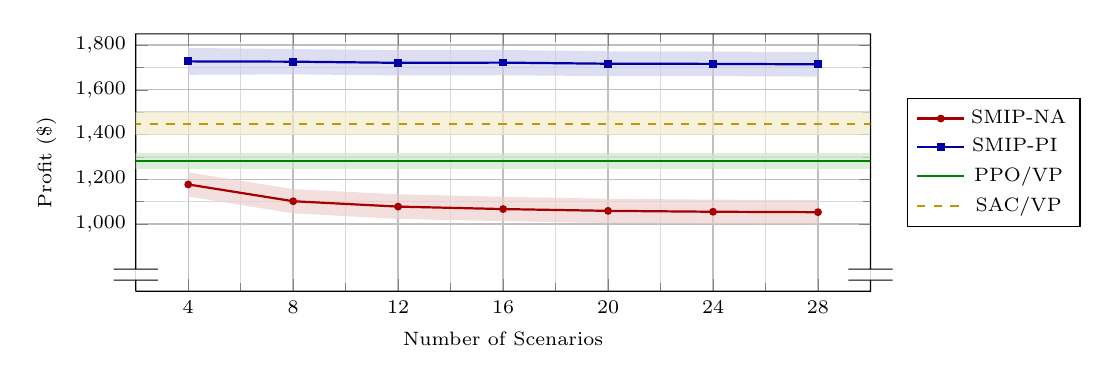
\begin{tikzpicture}
    \begin{axis}[
        width=0.9\textwidth,
        height=0.40\textwidth,
        xlabel={Number of Scenarios},
        ylabel={Profit (\$)},
        legend style={font=\scriptsize,
        at={(1.05,0.5)},  anchor=west,
        legend columns=1,         align=left},
        % under: legend style={font=\scriptsize, at={(0.5,-0.3)}, anchor=north, legend columns=3},
        tick label style={font=\scriptsize},
        label style={font=\scriptsize},
        grid=both,
        minor tick num=1,
        major grid style={line width=.5pt,draw=gray!50},
        minor grid style={line width=.5pt,draw=gray!30},
        ymajorgrids=true,
        yminorgrids=true,
        xtick={0,4,8,...,64},
        xmin=2, xmax=30,
        ymin=700, ymax=1850,
        ytick={1000,1200,..., 1800},
        axis y discontinuity=parallel, % Adds a break in the y-axis
        set layers,
    ]
    SMIP-NA Objective Value
    \addplot[
        color=darkred,
        mark=*,
        mark size=1,
        line width=.8pt
    ] coordinates {
        (4,1177) (8,1102) (12,1078) (16, 1067) (20,1059) (24,1055) (28,1053.02)
    };
    \addlegendentry{SMIP-NA};
        % SMIP-PI Objective Value
    \addplot[
        color=darkblue,
        mark=square*,
        mark size=1,
        line width=.8pt
    ] coordinates {
        (4,1726.94) (8,1725.61) (12,1720.46) (16,1721.39) (20,1716.40) (24,1715.75) (28,1713.73)
    };
    \addlegendentry{SMIP-PI };
    % PPO Objective Value
    \addplot[
        color=darkgreen,
        line width=.8pt
    ] coordinates {
        (0,1283) (40,1283)
    };
    \addlegendentry{PPO/VP};
    % SAC Objective Value
    \addplot[
        dashed,
        color=darkyellow,
        line width=.8pt
    ] coordinates {
        (0,1448) (40,1448)
    };
    \addlegendentry{SAC/VP};
    % Confidence intervals for SMIP-NA
    \addplot[name path=lower_na, draw=none] coordinates {
        (4,1123) (8,1048) (12,1023) (16,1013) (20,1004) (24,1001) (28,999)
    };
    \addplot[name path=upper_na, draw=none] coordinates {
        (4,1231) (8,1156) (12,1133) (16,1122) (20,1113) (24,1109) (28,1107)
    };
    \addplot[darkred!20, opacity=0.65] fill between[of=upper_na and lower_na];
    % Confidence intervals for SMIP-PI
    \addplot[name path=lower_pi, draw=none] coordinates {
        (4,1667) (8,1669) (12,1664) (16,1665) (20,1661) (24,1661) (28,1659)
    };
    \addplot[name path=upper_pi, draw=none,] coordinates {
        (4,1787) (8,1782) (12,1777) (16,1778) (20,1772) (24,1771) (28,1768)
    };
    \addplot[darkblue!20, opacity=0.65] fill between[of=upper_pi and lower_pi];
    % Confidence intervals for PPO
    \addplot[name path=lower_na, draw=none] coordinates {
        (0,1247) (30,1247)
    };
    \addplot[name path=upper_na, draw=none] coordinates {
        (0,1318) (30,1318)
    };
    \addplot[darkgreen!20, opacity=0.70] fill between[of=upper_na and lower_na];
    % Confidence intervals for SAC
    \addplot[name path=lower_na, draw=none] coordinates {
        (0,1397) (30,1397)
    };
    \addplot[name path=upper_na, draw=none] coordinates {
        (0,1499) (30,1499)
    };
    \addplot[darkyellow!20, opacity=0.70] fill between[of=upper_na and lower_na];
    \end{axis}
\end{tikzpicture}
\caption{Profit with 95\% CI across scenario sizes on 30 instances.}

\label{fig:objective_values}
\end{subfigure}

% Subfigure (b): Computational Time Plot
\begin{subfigure}[ht]{0.48\textwidth}
\centering
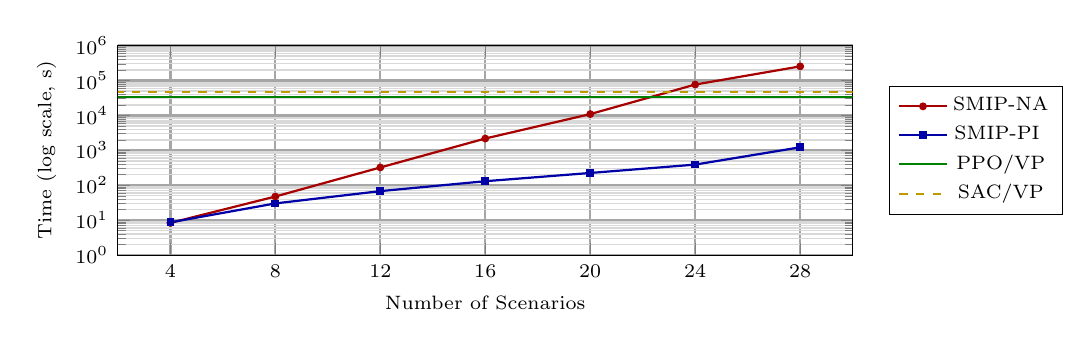
\begin{tikzpicture}
    \begin{axis}[
        width=0.9\textwidth,
        height=0.35\textwidth,
        xlabel={Number of Scenarios},
        ylabel={Time (log scale, s)},
        ymode=log, % Logarithmic scale for y-axis
        legend style=
        {font=\scriptsize,
        at={(1.05,0.5)},  
        anchor=west,
        legend columns=1,
        align=left            
        },
        % under: legend style={font=\scriptsize, at={(0.5,-0.3)}, anchor=north, legend columns=3},
        tick label style={font=\scriptsize},
        label style={font=\scriptsize},
        grid=both, % Show both major and minor grid lines
        major grid style={line width=.8pt, draw=gray!70}, % Thicker and darker for major grid
        minor grid style={line width=.5pt, draw=gray!30}, % Lighter for minor grid
        ymajorgrids=true,
        yminorgrids=true,
        xtick={0,4,...,64},
        xmin=2, xmax=30,
        ymin=1, ymax=1000000,
        ytick={1, 10, 100, 1000, 10000, 100000, 1000000},
        yticklabels={$10^{0}$, $10^{1}$, $10^{2}$, $10^{3}$, $10^{4}$, $10^{5}$, $10^{6}$},
    ]
    % SMIP-NA Computational Time
    \addplot[
        color=darkred,
        mark=*,
        mark size=1,
        line width=.8pt
    ] coordinates {
        (4,8.40) (8,47.70) (12,323.70) (16, 2181.00) (20,10905) (24,76442.7) (28,253037.4)
    };
    \addlegendentry{SMIP-NA};
    % SMIP-PI Computational Time
    \addplot[
        color=darkblue,
        mark=square*,
        mark size=1,
        line width=.8pt
    ] coordinates {
        (4,8.70) (8, 30.30) (12,  68.10) (16,  130.80) (20, 225.30) (24, 391.20) (28, 1222.50)
    };
    \addlegendentry{SMIP-PI };
    % DRL Training Time
    \addplot[
        color=darkgreen,
        line width=.8pt
    ] coordinates {
        (0,33085.9) (40,33085.9)
    };
    \addlegendentry{PPO/VP}
    % DRL Training Time
    \addplot[
        dashed,
        color=darkyellow,
        line width=.8pt
    ] coordinates {
        (0,47988.6) (40,47988.6)
    };
    \addlegendentry{SAC/VP}
    \end{axis}
\end{tikzpicture}
\caption{Total computational time across scenario sizes of 30 instances.}
\label{fig:computational_times}
\end{subfigure}

\begin{subfigure}[ht]{0.48\textwidth}
\centering
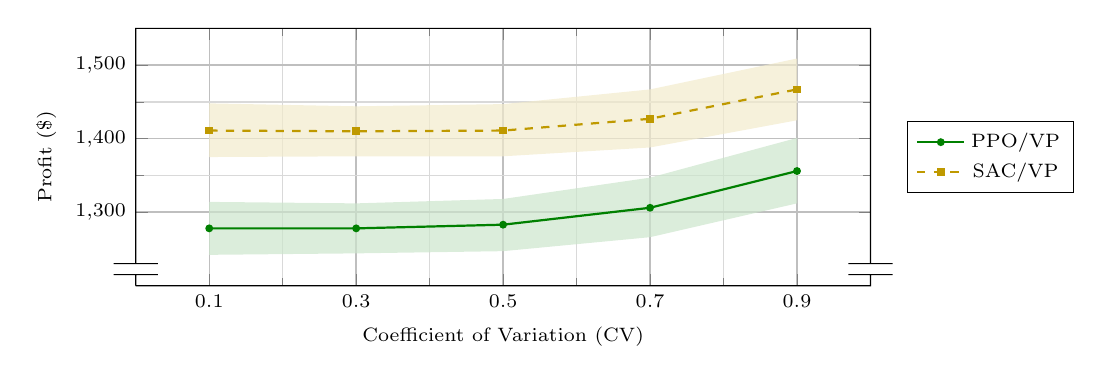
\begin{tikzpicture}
\begin{axis}[
    width=0.9\textwidth,
    height=0.40\textwidth,
    xlabel={Coefficient of Variation (CV)},
    ylabel={Profit (\$)},
    legend style={font=\scriptsize,
    at={(1.05,0.5)},  anchor=west,
    legend columns=1, align=left},
    tick label style={font=\scriptsize},
    label style={font=\scriptsize},
    grid=both,
    minor tick num=1,
    major grid style={line width=.5pt,draw=gray!50},
    minor grid style={line width=.5pt,draw=gray!30},
    ymajorgrids=true,
    yminorgrids=true,
    xtick={0.1,0.3,0.5,0.7,0.9},
    xmin=0, xmax=1,
    ymin=1200, ymax=1550,
    ytick={1300,1400,1500},
    axis y discontinuity=parallel, % Adds a break in the y-axis
]
% PPO/VP
\addplot[
    color=darkgreen,
    mark=*,
    mark size=1,
    mark options={solid},
    line width=.8pt
] coordinates {
    (0.1, 1278) (0.3, 1278) (0.5, 1283) (0.7, 1306) (0.9, 1356)
};

\addlegendentry{PPO/VP};

% SAC/VP
\addplot[
    dashed,
    color=darkyellow,
    mark=square*,
    mark size=1,
    mark options={solid},
    line width=.8pt
] coordinates {
    (0.1, 1411) (0.3, 1410) (0.5, 1411) (0.7,1427) (0.9, 1467)
};
\addlegendentry{SAC/VP};

% PPO-1
\addplot[name path=lower_ci, draw=none] coordinates {
    (0.1, 1242) (0.3, 1244) (0.5,  1247) (0.7, 1266) (0.9, 1312)
};
\addplot[name path=upper_ci, draw=none] coordinates {
    (0.1, 1314) (0.3, 1312) (0.5, 1318) (0.7, 1347) (0.9, 1401)
};
\addplot[darkgreen!20, opacity=0.70] fill between[of=upper_ci and lower_ci];

% SAC-1
\addplot[name path=lower_ci, draw=none] coordinates {
    (0.1, 1375) (0.3, 1376) (0.5, 1376) (0.7, 1388) (0.9, 1425)
};
\addplot[name path=upper_ci, draw=none] coordinates {
    (0.1, 1448) (0.3, 1444) (0.5, 1447) (0.7, 1467) (0.9,1509)
};
\addplot[darkyellow!20, opacity=0.70] fill between[of=upper_ci and lower_ci];

\end{axis}
\end{tikzpicture}
\caption{Profit with 95\% CI across CV levels on 30 unseen instances.}
\label{fig:demand_uncertainty}
\end{subfigure}
\caption{Sensitivity analysis of scenario size and demand spread.}
\label{fig:comparison_subfigures}
\end{figure}

\section{Conclusion and Future Directions}
This work introduces a novel MDP formulation for the MPP under demand uncertainty, incorporating realistic inequality constraints. We train an AM policy using actor-critic DRL methods with differentiable feasibility projections to construct MPP solutions. Experimental results demonstrate that our policy efficiently generates adaptive and feasible solutions, significantly outperforming baseline DRL methods and the SMIP-NA. This approach establishes an AI-driven decision-support policy for planning under uncertainty in a critical part of the global supply chain. Future work will extend the MPP formulation and scale to larger vessels and longer voyages, further enhancing the representativeness.

\clearpage

% \section{Acknowledgements}

\section*{Ethical Statement}
Human oversight is critical in decision-support tools to ensure fairness, accountability, and transparency. While models can enhance decision-making, they must not replace human judgment, particularly in high-stakes applications. We strongly encourage safeguards to mitigate automation bias, ensuring that users can override or challenge outputs, with continuous validation and auditing to uphold trust and fairness.

% \bibliographystyle{plain}
% %%%% ijcai25.tex

\typeout{IJCAI--25 Instructions for Authors}

% These are the instructions for authors for IJCAI-25.

\documentclass{article}
\pdfpagewidth=8.5in
\pdfpageheight=11in

% The file ijcai25.sty is a copy from ijcai22.sty
% The file ijcai22.sty is NOT the same as previous years'
\usepackage{ijcai25}

% Use the postscript times font!
\usepackage{times}
\usepackage{soul}
\usepackage{url}
\usepackage[hidelinks]{hyperref}
\usepackage[utf8]{inputenc}
\usepackage[small]{caption}
\usepackage{graphicx}
\usepackage{amsmath}
\usepackage{amsthm}
\usepackage{amssymb}
\usepackage{booktabs}
\usepackage[table,xcdraw]{xcolor}
\usepackage{algorithm}
\usepackage{algorithmic}
\usepackage[switch]{lineno}

\usepackage{xcolor}
\usepackage{subcaption} % For subfigures


% Comment out this line in the camera-ready submission
%\linenumbers

\urlstyle{same}

% the following package is optional:
%\usepackage{latexsym}

% See https://www.overleaf.com/learn/latex/theorems_and_proofs
% for a nice explanation of how to define new theorems, but keep
% in mind that the amsthm package is already included in this
% template and that you must *not* alter the styling.
\newtheorem{example}{Example}
\newtheorem{theorem}{Theorem}
\newtheorem{definition}{Definition}
\newtheorem{proposition}{Proposition}
\newtheorem{remark}{Remark}

% Following comment is from ijcai97-submit.tex:
% The preparation of these files was supported by Schlumberger Palo Alto
% Research, AT\&T Bell Laboratories, and Morgan Kaufmann Publishers.
% Shirley Jowell, of Morgan Kaufmann Publishers, and Peter F.
% Patel-Schneider, of AT\&T Bell Laboratories collaborated on their
% preparation.

% These instructions can be modified and used in other conferences as long
% as credit to the authors and supporting agencies is retained, this notice
% is not changed, and further modification or reuse is not restricted.
% Neither Shirley Jowell nor Peter F. Patel-Schneider can be listed as
% contacts for providing assistance without their prior permission.

% To use for other conferences, change references to files and the
% conference appropriate and use other authors, contacts, publishers, and
% organizations.
% Also change the deadline and address for returning papers and the length and
% page charge instructions.
% Put where the files are available in the appropriate places.


% PDF Info Is REQUIRED.

% Please leave this \pdfinfo block untouched both for the submission and
% Camera Ready Copy. Do not include Title and Author information in the pdfinfo section
\pdfinfo{
/TemplateVersion (IJCAI.2025.0)
}

\title{The Combined Problem of Online Task Assignment and Lifelong Path Finding\\ in Logistics Warehouses: A Case Study}


% Single author syntax
%\author{
%    Author Name
%    \affiliations
%    Affiliation
%    \emails
%    email@example.com
%}

%\author{Anonymous}

% Multiple author syntax (remove the single-author syntax above and the \iffalse ... \fi here)
%\iffalse
\author{
Fengming Zhu$^1$
\and
Fangzhen Lin$^1$
\and
Weijia Xu$^2$
\And
Yifei Guo$^2$\\
\affiliations
$^1$CSE Department, HKUST\\
$^2$Meituan Academy of Robotics Shenzhen\\
\emails
fzhuae@connect.ust.hk,
flin@cse.ust.hk,
\{xuweijia, guoyifei02\}@meituan.com
}
%\fi

\begin{document}

\maketitle

%\vspace{-3mm}

\begin{abstract}
%We study the online problem of task assignment and path finding in modern automated warehouses, which has significant applications in the logistics industry.
%%%% what assumption
%%The existing literature mostly considers ideal abstractions of such problems by imposing potentially unrealistic assumptions.
%%To this end, we propose a system that aims at mitigating those gaps between simulation and real-world deployment.
%%%%
%%The combined problem of task assignment and path finding for robot swarms is one of the key challenges in modern automated warehouses, especially in the logistics .
%The existing literature 
%(1)~mostly considers idealized formulations of such problems by assuming
%robot models that neglect rotational costs and focusing on well-formed layouts,
%and (2)~has not fully explored the benefit of deliberate task assignment.
%To address the above issues, our proposed system redesigns these two modules, namely
%(i)~a lifelong path planner that is directly tailored for a more practical robot model in possibly \textit{non}-well-formed layouts, and
%%(ii)~online task assignment that reacts on real-time states.
%(ii)~an task assigner that can adapt to the underlying path planner.
%Simulation experiments conducted in warehouse scenarios at \textit{Meituan}, one of the largest shopping platforms in China, demonstrate that
%(a)~\textit{in terms of time efficiency},
%our system takes only 83.77\% of the execution time needed for the currently deployed system at Meituan, outperforming other SOTA algorithms by 8.09\%;
%(b)~\textit{in terms of economic efficiency},
%ours can achieve the same throughput with only 60\% of the agents of the current scale.
%%%%
%% Simulation experiments conducted in warehouse scenarios at \textit{Meituan}, one of the biggest shopping platforms in China, demonstrate that our system, in terms of throughput, 
%% outperforms other SOTA algorithms by 10.2\%, and outperforms the currently deployed system at Meituan by 19.4\%.
%% From the economical side, our system can achieve the same throughput with only 60\% agents of the current scale.
%%%%
%Our observations also imply that rule-based methods, though may not be general, are sometimes effective enough in practice.




We study the combined problem of online task assignment and lifelong path finding, which is crucial for the logistics industries.
However, most literature either (1) focuses on lifelong path finding assuming a given task assigner, or (2) studies the offline version of this problem where tasks are known in advance.
We argue that, to maximize the system throughput, the online version that integrates these two components should be tackled directly.
To this end, we introduce a formal framework of the combined problem and its solution concept.
Then, we design a rule-based lifelong planner under a practical robot model that works well even in environments with severe local congestion.
Upon that, we automate the search for the task assigner with respect to the underlying path planner.
Simulation experiments conducted in warehouse scenarios at \textit{Meituan}, one of the largest shopping platforms in China, demonstrate that
(a)~\textit{in terms of time efficiency},
our system requires only 83.77\% of the execution time needed for the currently deployed system at Meituan, outperforming other SOTA algorithms by 8.09\%;
(b)~\textit{in terms of economic efficiency},
ours can achieve the same throughput with only 60\% of the agents currently in use.
\end{abstract}



\section{Introduction}

%% background problem
%We consider the problem of real-world warehouse automation, where a fleet of robots are programmed to pick up and deliver packages without any collision.
%The investigation of such a problem will significantly benefit logistics companies. 
%However, the problem is inherently hard, primarily for two reasons:
%(1)~the computational complexity of multi-agent path finding is notorious especially when the size of the robot fleet is considerably large, and
%(2)~the stream of tasks arrive in an online fashion of which the accomplishment also depends on the subsequent execution by the path finding module. 

% Lin's version
We consider the problem present in highly automated real-world warehouses where a fleet of robots is programmed to pick up and deliver packages without any collision.
This is a significant problem for logistics companies as it has a major impact on their operational efficiency.  
It is a difficult problem for at least the following  two reasons:
(1)~the computational complexity of multi-agent path finding is notoriously high, especially when the number of robots is large, and
(2)~the dynamic and real-time assignment of tasks to the robots both depends on and affects the subsequent path finding.


% Existing mainstream solutions and main issues
There is a vast literature that studies idealized abstractions of such real-world problems.
The most commonly seen formulation is to assume a given (or naive) task assigner, and therefore, the focus is merely on the path-finding part, which is usually termed as one-shot \textit{Multi-Agent Path Finding} (MAPF)~\cite{yu2013structure,erdem2013general,sharon2015conflict,li2021eecbs,okumura2022priority,okumura2023lacam}
or its lifelong version \textit{Multi-Agent Pickup and Delivery} (MAPD)~\cite{ma2017lifelong,vsvancara2019online,li2021lifelong,okumura2022priority}.
%Note that a task assigner tightly depends on the underlying path finding. In other words, to maximize the throughput of the whole pipeline, one should adapt a task assigner to a path planner.
However, to maximize the throughput of the whole production pipeline, the task assigner should also be deliberately designed with respect to the particular underlying path planner.
To this end, some recent work has further investigated the combined problem of \textit{Task Assignment and Path Finding} (TAPF)~\cite{yu2013multi,ma2016optimal,honig2018conflict,liu2019task,chen2021integrated,tang2023solving}.
%Nevertheless, this line of work is mostly restricted to  offline scenarios, i.e., tasks (and/or their release times) are priorly known.
Nevertheless, this line of work is mostly restricted to  offline scenarios, i.e., tasks (and/or their release times) are assumed to be known.
%However, so far only offline scenarios, i.e. tasks (and/or their release times) are assumed upfront, are considered.
In practice, for example in a sorting center, orders may come dynamically in real-time.

% Other implementation-related problems
Besides, we draw attention to two seemingly minor but indeed fundamental aspects.
\textbf{For one}, the robots are usually abstracted to agents doing unit-cost unit-distance cardinal actions,
i.e., \{\texttt{stop}, \texttt{$\uparrow$}, \texttt{$\downarrow$}, \texttt{$\leftarrow$}, \texttt{$\rightarrow$}\}, what we term as the \texttt{Type}$\oplus$ robot model.
The planned paths are later post-processed to executable motions regarding kinematic constraints~\cite{honig2016multi} and action dependencies~\cite{honig2019persistent}, as a real-world robot has to rotate before going in a different direction.
Imaginably, when the rotational cost is not negligible compared to the translational cost, the quality of the plans computed for the \texttt{Type}$\oplus$ robot model will be largely compromised when instantiated to motions.
A candidate solution is to revisit and reimplement the existing algorithms over an alternative set of atomic actions \{\texttt{stop}, \texttt{forward}, \texttt{$\circlearrowright$90}, \texttt{$\circlearrowleft$90}\}, which we advocate in this paper as the \texttt{Type}$\odot$ robot model.
\textbf{For another}, most of the literature assumes the problem instance to be \textit{well-formed}~\cite{ma2017lifelong,liu2019task,xu2022multi} to guarantee completeness of their methods, which is actually a strong condition requiring that every agent can find a collision-free path to her current goal even if the others are stationary.
%In fact, \textit{non-well-formed} instances are also commonly seen in modern warehouse, illustrated as an example in Figure~\ref{fig:eg_non_wf}.
%The planner that we will present later makes no use of this potentially unrealistic assumption.
However, this assumption is often not met in modern warehouses. In particular, the instance (Figure~\ref{fig:eg_non_wf}) that we consider in this work does not satisfy this condition.

%wellformed instance too strong!

%\textit{
%Given a potentially non-well-formed layout with the number of agents varying,
%is there a good way for online TAPF that can take the advantage of the layout.
%}
%\textbf{That is why this is a case study}


%Might be minor for academia, but critical for industrial deployment

%MAPF-POST and Temporal Plan Graph (TPG) ~\cite{honig2016multi}

%allow task swapping~\cite{okumura2023solving}

%robust warehouse execution~\cite{honig2019persistent}

%capacitated mapd~\cite{chen2021integrated}

%probably no need for a general algorithm, but a practical one for certain structured layouts


\begin{figure*}[tb]
\centering
\vspace{-3mm}
\includegraphics[width=180mm]{fig/warehouse3-compressed}
\caption{A \textit{non-well-formed} instance 
%(see~\protect\cite{xu2022multi}) 
currently deployed in Meituan warehouses. The white cells near \textsc{Green} dots are delivery ports, while the ones near \textsc{Red} dots are pickup ports. Colored circles heading to different directions with numbers are agents. The colored box (blue) is a pickup port currently assigned to the agent in the same color (ID 45 in the lower right area). Congestion happens a lot near the pickup ports.}
\vspace{-1mm}
\label{fig:eg_non_wf}
%\vspace{-2mm}
\end{figure*}

% Our Contribution
Considering the aforementioned issues,
%we here propose a system that organically integrates the task assignment and the path planning in an online manner.
%so that the mismatch between algorithmic simulation and real-world deployment shall be alleviated. 
we introduce a formal framework to study the combined problem that organically integrates task assignment and path finding in an online manner.
%\textcolor{red}{Rigorously formalize the online problem}
%More specifically,
To solve the formalized problem,
we \textbf{first} develop lifelong path finding algorithms directly for the \texttt{Type}$\odot$ robot model (assuming an arbitrary task assigner), including those adapted from the existing literature and our new rule-based planner which performs both efficiently and effectively, even for non-well-formed instances.
%Note that an additional strong assumption of the aforementioned work is that the layout should better be \textit{well-formed}~\cite{ma2017lifelong},
%which is dropped in our system, since non-well-formed layouts are commonly seen in modern warehouses.
%We illustrate a non-well-formed example in Figure~\ref{fig:eg_non_wf}.
\textbf{Secondly}, we propose a novel formulation that addresses the online problem of task assignment as optimally solving a Markov Decision Process~(MDP), with path planners as hyper-parameters.
Due to the complex state space and transition of the formulated MDP, we resort to approximated solutions by reinforcement learning (RL), as well as other non-trivial rule-based ones with insightful observations.
%To our best knowledge, this is the first compound system that directly tackles both task assigner and path planner simultaneously in an online fashion.
\textit{Simulation experiments on warehouse scenarios at Meituan, one of the largest shopping platforms in China, have shown that our system
(1)~takes only 83.77\% of the execution time needed for the currently deployed system at Meituan, outperforming other SOTA algorithms by 8.09\%; and
(2)~can achieve the same throughput with only 60\% of the agents of the current scale.}
We also draw an important lesson from this study
that both path finding and task assignment should fully exploit the warehouse layout, as it is normally fixed in a relatively long period of time after deployment, though the number of agents may still vary.
To this end, it might be more worthwhile to investigate layout-dependent-agent-independent solutions instead of entirely general-purpose solutions.




This paper is organized as follows.
We first list a few related areas in Section~\ref{sec:related}.
Then the problem formulation is provided in Section~\ref{sec:problem}.
We later present our system in two parts: the path planners in Section~\ref{sec:pf}, and the task assigners in Section~\ref{sec:ta}.
Experimental results are shown in Section~\ref{sec:exp}, mainly conducted for Meituan warehouse scenarios with various scales of agents.
We conclude the paper with a few insightful discussions in Section~\ref{sec:conclusion}.

% Our system


% Organization


\section{Related Work}
\label{sec:related}
%Our work pertains to a broad range of research areas, mainly on planning from the multi-agent community and scheduling from the operations research community.

% 1. path finding
% MA-PF/PD
\textbf{Path Finding.}
The study of MAPF aims to develop centralized planning algorithms.
In spite of the computational complexity being NP-hard in general~\cite{yu2013structure},
researchers have developed practically fast planners that can even solve instances with hundreds of agents within seconds.
Exemplars can be found via reduction to logic programs~\cite{erdem2013general},
prioritized planning~\cite{silver2005cooperative,ma2019searching,okumura2022priority},
conflict-based search~\cite{sharon2015conflict,li2021eecbs}, 
depth-first search~\cite{okumura2023lacam}, etc.
Most of them can be extended to the online version of the problem, i.e. MAPD,
where the goals assigned to agents are priorly unknown~\cite{ma2017lifelong,vsvancara2019online,li2021lifelong}.
%Usually, adaptations are then made via communication between robots and broadcasting by the central controller for the purpose of synchronization.
%A notable drawback is that both MAPF and MAPD assume a task assigner should be given.


% 2. task assignment
% TAPF, Anon-MAPF
% Multi-Goal MA-PF/PD
\textbf{Task Assignment.}
The earliest attempt is the formulation of \textit{Anonymous}-MAPF (AMAPF) that does not specify the exact goal that an agent must go to~\cite{stern2019multi}.
%, but the total number of anonymous goals should be less than or equal to the number of agents
Compared with the labeled version, AMAPF can be solved in polynomial time,
via reduction to max-flow problems~\cite{yu2013multi}, or target swaps~\cite{okumura2023solving}.
As a generalization,
TAPF explicitly associates each agent with a team~\cite{ma2016optimal}, or with a set of candidate goals~\cite{honig2018conflict,tang2023solving},
and eventually computes a set of collision-free paths as well as the corresponding assignment matrix.
Another analogous formulation is called \textit{Multi-Goal} (MG-)MAPF~\cite{surynek2021multi,ijcai2024p0028} and its lifelong variant MG-MAPD~\cite{xu2022multi}, which also associates each agent with a set of goals, but the visiting order is pre-specified.
%Imaginably, the further generalized model should consider that tasks arrive as a priorly unknown sequence and are assigned to agents for real-time path finding.
%To the best of our knowledge, this problem is so far open,
%for which we will present a solution system in this paper.

%Hungarian method~\cite{kuhn1955hungarian}
%allow task swapping~\cite{okumura2023solving}

%% 3. comb. opt., scheduling 
%% Job shop scheduling, vehicle routing
%\textbf{Scheduling.}
%One may notice the analogy between TAPF and job-shop scheduling problems (JSSP)~\cite{manne1960job,jain1999deterministic} or vehicle routing problems (VRP)~\cite{toth2014vehicle,braekers2016vehicle}.
%However, there are two key differences: (1) job durations in JSSP and route lengths in VRP are usually known in advance and (2) the execution of jobs or routes are independent of each other.
%Neither of the two conditions holds in TAPF, especially when the tasks are released online.

%\textcolor{red}{some postponed to Appendix~\ref{apd:more_related_work}}
\textit{We also append some discussion on other less related areas to Appendix~\ref{apd:more_related_work}.}
Despite the rich literature, none of the above directly solves the online problem that a real-world automated warehouse is faced with, which well motivates this work.



\section{Problem Definition}
\label{sec:problem}

%\textcolor{red}{N as a number and a set}

We consider a set of agents $N$, moving along a 4-neighbor grid map given as an undirected graph $G = (V, E)$,
where $V$ is the set of vertices and $E$ is the set of unit-cost edges.
Let $P, D\subseteq V$ denote the set of pickup ports and the set of delivery ports, respectively.
Usually, these two sets are disjoint and are specified alongside the map graph.


Let $k$ starting from 0 denote any arbitrary timestep (to be distinguished from the later notations of tasks).
At each timestep $k$, the local \textit{agent-state} of agent $i$, denoted as $\phi_i^k$, is a 3-tuple consisting of
her current location $l_i^k\in V$,
direction $d_i^k\in \{n,s,w,e\}$,
and goal $g_i^k \in P\cup D$.
$\Phi_i$ is the set of all possible local states of agent $i$, and consequently $\Phi = \prod_{i\in N} \Phi_i$ is the set of all possible \textit{joint agent-states}.
Each agent is associated with a set of four unit-cost actions $A=\{\texttt{stop}, \texttt{forward}, \texttt{$\circlearrowright$90}, \texttt{$\circlearrowleft$90}\}$ (called the \texttt{Type}$\odot$ robot model), with their usual meaning specified using the deterministic function $move$.
For example,
\[
\begin{split}
	move(((3,28), w),\ \ \ \ \ \ \ \ \ \texttt{$\circlearrowright$90}) &\to ((3,28), n) \\
	move(((3,28), e), \texttt{forward}) &\to ((3,29), e)
\end{split}
\]
While planning paths for agents, we need to avoid the following types of collisions.
\begin{definition}[Collision types~\cite{stern2019multi}]
Let $i$ and $j$ be any arbitrary pair of agents,
	\begin{itemize}
		\item Vertex-collision: $l_i^k = l_j^k$,
		\item Edge-collision: $l_i^k = l_j^{k+1} \land l_j^{k} = l_i^{k+1}$,
%		\item Following-conflict: $l_i(k+1) = l_j(k)$.
	\end{itemize}
\end{definition}

%In fact, there is an additional type of conflicts, namely \textit{cycle-conflict}, which is a special case when the group of agents that run into a following-conflict form a cycle.
%Mathematically, a cycle-conflict happens when there exists a subset of agents
%$\{i, i+1, \cdots, j-1, j\}$,
%such that $l_i(k+1) = l_{i+1}(k)\land l_{i+1}(k+1) = l_{i+2}(k)\land \cdots\land l_{j}(k+1) = l_{i}(k)$.
%Note that we do not explicitly include cycle-conflicts in our discussion because forbidding following-conflicts implies forbidding cycle-conflicts.

%\begin{definition}[Lock types]
%ss
%	\begin{itemize}
%		\item Dead-lock.
%		\item Live-lock.
%	\end{itemize}
%\end{definition}

%The so-called tasks are composed of a sequence $I$ of typed items. 
%The type of an item $\iota \in I$ is also known as a \textit{stock keeping unit}\footnote{https://en.wikipedia.org/wiki/Stock\_keeping\_unit} (SKU).
%We let $T$ denote the set of all possible types (SKUs).
The so-called tasks are composed of a sequence $I$ of typed items. 
Each item $\iota \in I$ is associated with a type $t\in T$.
A back-end demand database specifies for each type a subset of delivery ports that items of the type need to be delivered to. 
Here we model such a database as a lookup table $L: T\mapsto 2^D$.
As $L$ will be changed in real-time, we also let $L^k$ denote the demand database at timestep~$k$.
When an agent has finished her last delivery job and returned to a pickup port at timestep $k$,
an item, say of type $t$, will be loaded onto this idle agent.
The system will then check the lookup table $L^k$, choose one target delivery port $g\in L^k(t)$ to assign to this agent, and delete this demand, i.e. $L^{k+1}(t) = L^k(t)\backslash \{g\}$.

Also, we have an assignment table $\eta$ that keeps track of which one of the loaded items is assigned to which agent, i.e., $\eta(\iota) = i$ means the item $\iota$ is currently carried by agent $i$.
An item $\iota$ is \textit{delivered} if there exists a timestep $k$ such that $l_{\eta(\iota)}^k = g_{\eta(\iota)}^k$, i.e., the agent carrying this item has reached her goal.
Upon successful delivery, the item $\iota$ will be deleted from the entry of $\eta$.
As $\eta$ is being changed  over time, we also use the time-indexed version $\eta^t$.
 
%Once an agent is assigned a goal, she cannot swap her goal with that of anyone else, as in real-world warehouses those robots are not equipped with arms and cannot swap packages.
We assume (1) $L$ has recorded the demands of a long enough period of time, and therefore, will not be enlarged;
and (2) an item will be appended to the system
only when it is loaded onto an agent.
%We also assume that no two agents simultaneously arrives at two pickup ports or two delivery ports due to the continuous-time nature of the real-world problem, but we allow the case when one is at a pickup port and the other is at a delivery port.
%Note that this does not imply any two agents will not appear simultaneously at the same location and hence no impossibility of any collisions.
%The above assumption is merely about no two agents will be switched to such a status waiting for assignment.

%(3)~no two agents arrive at their pickup ports simultaneously.
%Therefore, the path planner has no knowledge of the forthcoming items and their types.

With the above notations, we formally define the dynamics of the whole system as a deterministic \textit{system-transition} function over \textit{system-states}.
\begin{enumerate}
	\item
	A \textit{system-state} $\psi$ is a tuple consisting of the joint agent-state $\phi = \{\phi_i\}_{i \in N}$, the lookup table $L$, and the assignment table $\eta$ at that moment. % illegal state?
	Let $\Psi$ denote all possible system states.
	Among them, there is an initial system-state $\psi^0 = (\phi_1^0, \cdots, \phi_N^0, L^0, \eta^0)$.
%	A system state is \textit{legal} if no two agents are at pickup locations simultaneously.
	
	\item
	The space of \textit{system-actions} is $\Omega = (A\cup P\cup D)^N$. That is, a \textit{system-action} $\omega\in \Omega$ is an ordered tuple of the atomic actions of agents where any of them can be substituted by an assignment decision.
	A system-action $\omega$ is \textit{executable} under a legal system-state $\psi$ iff
	\[
	\begin{split}
	 \forall i \in N.\ 
	 & [\l_i \in V\backslash (P\cup D) \land \omega_i \in A] \lor \\
	 & [\l_i \in P \land \omega_i \in D] \lor
	[\l_i \in D \land \omega_i \in P]
	\end{split}
	\]
	
	\item $\Gamma: \Psi \times \Omega \mapsto \Psi$ is the \textit{system-transition} function, which means (1) if no agents are at the pickup/delivery ports, then the system proceeds by deterministically moving agents by their reported actions, which will not change the goal component $g_i$ in each agent-state $\phi_i$; or (2) if any agent arrives at any pickup (resp. delivery) port, then the  system  needs to re-assign the agent the next delivery (resp. pickup) port, which will change the goal of that particular agent to the corresponding new location and temporarily force her to stay in-place, and change the demand table $L$ as well as the assignment table $\eta$ accordingly.
\end{enumerate}
%\textcolor{red}{one item at a time}
An additional minor assumption is, even if two agents arrive at two different pickup (resp. delivery) ports simultaneously,
%they will not be ``switched'' to the status of waiting for new-delivery (resp. pickup) assignments asimultaneously, as in real-world both time and motion execution are continuous.
they will eventually get assigned certain new ports within the next one single timestep one by one in a random order. We do not care about the case where one is waiting for a new-delivery assignment while another is waiting for a new-pickup assignment.

In summary, a \textit{problem instance} is a following tuple $$<N, G, P, D, A, I, L>,$$
and consequently a \textit{principle solution} is threefold:
\begin{enumerate}
	\item $\pi_N: \Phi\mapsto A^N$ is the routing policy that outputs the next action for each agent given their current states. It is unnecessary to compute the entire $\pi_N$ completely upfront, instead, execution can be interleaved with replanning.
	\item $\pi_{D}: \Psi \times 2^D \mapsto D$ is the delivery selection policy which assigns an agent a delivery port among the candidates according to $L(t)$ when she is at one of the pickup ports and given an item of type $t$.
%	Note that $t$ is not one of the input parameters as the loaded item is not within control. 
	\item $\pi_{P}: \Psi \mapsto P$ is the pickup selection policy which assigns an agent a pickup port to return to when she has finished the delivery.
\end{enumerate}
Note that (1) both $\pi_D$ and $\pi_P$ assign one new goal at a time, as we assumed before;
(2) both $\pi_D$ and $\pi_P$ will change the goal of that particular agent to the corresponding port,
while $\pi_N$ will not;
(3) if an agent is at a pickup or delivery port, then her agent-action, even if specified by $\pi_N$, will be overwritten to $\texttt{stop}$ by the decision of $\pi_D$ or $\pi_P$.

%condition for feasible policy%
\begin{definition}[Feasibility]
Given any system-state $\psi$ and the system-transition $\Gamma$, the application of the above solution policy $(\pi_N, \pi_D, \pi_P)$ deterministically outputs a successor system-state $\psi'$. If there is no aforementioned collision between $\psi$ and $\psi'$, then $(\pi_N, \pi_D, \pi_P)$ is a feasible solution.
\end{definition}

%A goal $g\in P\cup D$ is reached under $\pi_N$ if there exists an agent $i$ and a timestep $k$, such that $l_i(k) = g$.
%An item of type $t$ is delivered if the target delivery port assigned by $\pi_{D}$ is reached. 

%TODO: two items with identical goals

%The system ends immediately once it has delivered every item in the online sequence $I$, in a given period of time.
We finally define \textit{makespan} as our evaluation metric.
\begin{definition}[Makespan]
	Given a problem instance with its initial system-state $\psi^0$, and a feasible solution $(\pi_N, \pi_D, \pi_P)$, an execution trajectory will be generated by the sequential applications of the solution policy $\{\psi^0, \psi^1, \cdots\}$. The makespan is the minimum timestep $k$ such that every item in I is delivered at $\psi^k$. 
\end{definition}

However, in real-world warehouses, the pickup ports are usually concentrated in a restricted local area for operational convenience, e.g., in the top right corner of Figure~\ref{fig:eg_non_wf}. Therefore, $\pi_{P}$ is normally implemented for the purpose of balancing the loads over all pickup ports.
\textbf{In this work, we merely aim at a \textit{practical solution} consisting of only $(\pi_N, \pi_D)$, assuming $\pi_{P}$ is given and is not part of the desired solution.}







%\textbf{Evaluation Protocol.}
%Since usually the underlying order database $\mathcal{T}$ is quite large, we will run the system through relatively small sets of tasks to test the elapsed \textit{makespans}, i.e., the number of timesteps to accomplish the given set of tasks.

%\begin{example}[System pipeline]
%As in Figure~\ref{fig:eg_non_wf},
%$\textsc{Robot}_1 \sim \textsc{Robot}_{50}$ initially rest in random locations upon the completion of the system execution the last time. Now the system is launched and every robot starts moving towards the pickup ports, namely $\textsc{Red}_1$ and $\textsc{Red}_2$. Suppose $\textsc{Robot}_{31}$ first reaches $\textsc{Red}_2$, the human operator loads one item, say a dozen of eggs, onto $\textsc{Robot}_{31}$, and the system checks the demand database and finds out that there are three orders requesting a dozen of eggs, with corresponding delivery ports $\textsc{Green}_{69}$, $\textsc{Green}_{142}$, and $\textsc{Green}_{83}$. After deliberate consideration, the system decides to send $\textsc{Robot}_{31}$ to $\textsc{Green}_{83}$ this time (and later ones to the remaining two delivery ports), and plans a path for $\textsc{Robot}_{31}$ to go from $\textsc{Red}_2$ to $\textsc{Green}_{83}$ while avoiding potential collisions with others, and so forth.
%\end{example}

\begin{example}[System pipeline]
As shown in Figure~\ref{fig:eg_non_wf}, $\textsc{Robot}_1 \sim \textsc{Robot}_{50}$ initially rest in random locations after the last system execution. Once the system is launched, each robot moves towards the pickup ports, $\textsc{Red}_1$ and $\textsc{Red}_2$. When $\textsc{Robot}_{31}$ reaches $\textsc{Red}_2$, the human operator loads a dozen eggs onto it. The system checks the demand database and finds three orders for a dozen eggs, with delivery ports $\textsc{Green}_{69}$, $\textsc{Green}_{142}$, and $\textsc{Green}_{83}$. After consideration, the system decides to send $\textsc{Robot}_{31}$ to $\textsc{Green}_{83}$ this time, planning a path while avoiding potential collisions, with subsequent deliveries to the other two ports.
\end{example}

One may see potential connections between our problem and the standard formulation MAPD in the existing literature, \textit{we postpone some remarks elaborating on the differences to Appendix~\ref{apd:relate_to_mapd}, due to the limited space}.
%\begin{remark}[Relation to MAPD]
%In MAPD, an online task $t_i$ is characterized by a pickup port $s_i$ and a delivery port $g_i$ with a priorly unknown release time. Once an agent becomes idle, she will select one task $t^* = (s^*, g^*)$ of her best interest from the released ones, and then plan a path from her current location to $g^*$ through $s^*$.
%Mapping to our settings, an agent becomes idle only when she arrives at a pickup port, and shall be assigned one delivery port from the candidate ones, say $\{g_1, \cdots, g_k\}$.
%Suppose the system will simply pair each delivery port with a pickup port immediately, for which the particular agent will return to after the delivery. Then it is equivalent to, in the language of MAPD, releasing $k$ tasks $\{(g_1, \pi_P(g_1)), \cdots, (g_k, \pi_P(g_k)\}$.
%However, after choosing one from the $k$ tasks and assigning it to an agent, the rest $(k-1)$ tasks will be temporarily removed, or say ``deactivated'', from the pool of released tasks until the next item of the same type arrives.
%\end{remark}


We clarify that in the rest of the paper, by ``path finding'' we mean to compute $\pi_N$, and by ``task assignment'' we mean to compute $\pi_D$.


\section{Path Finding}

\label{sec:pf}

In this section, we first review several representative algorithms that can plan collision-free paths in a lifelong fashion.
However, they are not always effective for resolving collisions under the \texttt{Type}$\odot$ robot model for non-well-formed instances like Figure~\ref{fig:eg_non_wf}.
To this end, we propose a simple-yet-powerful rule-based planner
%that takes advantage of the map layout,
 which is capable of efficiently and robustly moving robots without collisions or deadlocks.

%\begin{definition}[Well-formed instance~\cite{xu2022multi}]
%	The vertices in $P\cup D$ are defined as task endpoints, while the initial locations of agents $\{l_i^0\}_{i \in N}$ are defined as non-task endpoints. A problem instance is well-formed iff (1)~the set of non-task endpoints is disjoint with the set of task endpoints, and (2)~there exists a path between any two endpoints that traverses no other endpoints.
%\label{def:wellform}
%\end{definition}

%\textcolor{red}{why this layout is hard}
%
%\textcolor{red}{not effective examples in Appendix~\ref{apd:pf_notgood_eg}}


\subsection{Existing Lifelong Path Finding Algorithms}

\textbf{Prioritized Planning.}
A straightforward way is to prioritize path finding for each agent by assigning them  distinct priorities, known as \textit{Cooperative A$^*$} (CA$^*$)~\cite{silver2005cooperative}, which can also be extended to lifelong situations.
In descending order of priority, the agents will plan their paths one by one.
Once an agent with a higher priority has found her path, those $(state, time)$ pairs along the path will be \textit{reserved} for this particular agent.
All subsequent agents with lower priorities will view those reservations as states that are unreachable at the corresponding timesteps, i.e. as spatio-temporal obstacles.
Therefore, each agent will need to conduct optimal search over the joint space of state and time.
Understandably,
there is a chance that an agent with a lower priority cannot compute any feasible path given the preceding path computed by a higher-priority, which makes the algorithm itself incomplete.
This situation is even worse under the \texttt{Type}$\odot$ robot model, as an agent often needs to rotate in-place before going to an adjacent vertex, which adds extra difficulty of avoiding collisions. \textit{An illustrative example is provided in Appendix~\ref{apd:pf_notgood_eg}}.

\textbf{Rolling Horizon Collision Resolution.}
A more systematic approach for lifelong path finding is to \textit{window} the search process~\cite{silver2005cooperative}.
This idea is further developed by~\cite{li2021lifelong} as 
the \textit{Rolling Horizon Collision Resolution} (RHCR) framework.
The framework takes two use-specified parameters: (1)~the replanning frequency $h$ and (2)~the length of the collision resolution window $w\geq h$, ensuring that no collisions occur within the next $w$ timesteps.
The framework is general enough to encompass most MAPF algorithms.
An example is to
extend conflict-based search (CBS)~\cite{sharon2015conflict,li2021eecbs} to the lifelong version using this RHCR framework, where the high-level constraint tree is expanded only if there are still collisions within the first $w$ timesteps, resulting in a much smaller constraint tree.
However, under the \texttt{Type}$\odot$ robot model, neighboring agents often require more timesteps to resolve collisions, especially in crowded local areas.
\textit{An example is provided in
Appendix~\ref{apd:pf_notgood_eg}.}

%
%\subsection{Prioritized Planning}
%
%A straightforward way of extending single-agent path finding to multi-agent path finding is to assign each agent a priority ordering, known as \textit{Cooperative A$^*$} (CA$^*$)~\cite{silver2005cooperative}.
%According to descending order of the priorities, the agents will plan their path one by one.
%Once an agent of a higher priority has found her path, those $(state, time)$ pairs along the path will be \textit{reserved} for this particular agent.
%All subsequent agents with lower priorities will see those reservations as states that are unreachable at corresponding timesteps, i.e. as spatio-temporal obstacles.
%In principle, each agent will need to conduct optimal search over the joint space of state-and-time, adding a bit overhead compared with optimal search over only states.
%
%% greedy
%
%Despite of being easy to implement and thus highly extendable, this paradigm is understandably incomplete, as it may not find any collision-free solution given a certain priority ordering whereas the problem instance is indeed solvable.
%A recent study~\cite{ma2019searching} also shows that there exists certain problem instances that are unsolvable for any order of static priorities.
%The authors therefore propose a method called \textit{Priority-Based Search} (PBS), which resembles the two-level method \textit{Conflict-Based Search} (CBS) but searches for a feasible priority ordering in its high level.
%
%\textcolor{red}{incomplete, if higher pri plans first while the lower one got no way to go}
%
%Note that all of the above mentioned algorithms assume that (1) each agent will serve as an obstacle when she reaches the goal, and (2) the system should terminate only when all agents arrives at their goals.
%Adaptations need to be made in situations of lifelong path finding, where agents are repeatedly assigned new goal locations.
%For decoupled algorithms like CA$^*$, one can easily reuse the reservation table for the previously planned paths, and plan new paths for the currently idle agents that are assigned new goals.
%For centralized algorithms like PBS, the central controller has to replan for \textit{all the agents} even if only one agent is assigned a new goal.
%% must be a different one from anyone else
%
%In this paper, we only implement the lifelong CA$^*$ for the \texttt{Type}$\odot$ robot model as one of the baselines of prioritized planning due to its flexibility, later denoted as \textbf{PP}.
%
%
%
%\subsection{Rolling Horizon Collision Resolution}
%A more systematic approach to extending one-shot MAPF algorithms to lifelong ones is to \textit{window} the search process~\cite{silver2005cooperative}.
%This idea is further developed by~\cite{li2021lifelong} as 
%the \textit{Rolling Horizon Collision Resolution} (RHCR) framework.
%The framework takes two use-specified parameters: (1)~the replanning frequency $h$ and (2)~the length of the collision resolution window $w$, ensuring $h \leq w$.
%The framework is general enough to encompass most of the MAPF algorithms, for example
%\begin{enumerate}
%	\item For CA$^*$, the state-time reservations made for the previously planned agents with higher priorities will only be effective within the first $w$ timesteps, and therefore, the size of the reservation table will reduce from $|states| \times T_{max}$ to $|states| \times w$. 
%	\item For CBS, the high-level contraint tree will be extended only if there are still collisions happening within the first $w$ timesteps, and therefore, the depth the constraint tree will be much smaller, similar for PBS.
%\end{enumerate}
%In this paper, we only implement RHCR upon CBS for our \texttt{Type}$\odot$ robot model due to 
%its completeness\footnote{CBS is complete for one-shot MAPF instances. Note that even with certain deadlock avoidance mechanisms mentioned in~\cite{li2021lifelong} the RHCR framework is still incomplete.} in theory, later denoted as \textbf{RHCR-CBS}.
%
%may need to reduce to $w\gets \infty$ when congestion around pickup ports
%

\subsection{Our Solution: Touring With Early Exit}



% traffic jam near pickup ports leads to failures or time-outs for the existing algorithms.




Instead of doing deliberate planning, we here present a simple-yet-effective rule-based planner, named \textit{Touring With Early Exit} (later denoted as \textbf{Touring} for short).
As summarized in Algorithm~\ref{alg:touring},
this planner consists of three main rules \textsc{Rule1-touring}, \textsc{Rule2-early-exit}, and \textsc{Rule3-safe}.
We will explain them one by one.

%\vspace{-3mm}
\begin{algorithm}[tb]
\small
    \caption{Touring with early exit}
    \label{alg:touring}
    \textbf{Input}: $states = (\{l_i\}_{i\in N}, \{d_i\}_{i\in N}, \{g_i\}_{i\in N})$\\
    \textbf{Parameter}: for any arbitrary timestep $k$, omitted below\\
    \textbf{Output}: next joint-action $actions$
    \begin{algorithmic}[1] %[1] enables line numbers
        \STATE $actions \gets \textsc{Rule1-touring}(states)$
        %\textcolor{red}{double-check}
        \IF{$\textsc{Exists-deadlock}(states)$}
        	\STATE $actions \gets \textsc{Rule3-safe}(states, actions)$
        	\STATE \textbf{return} actions
        \ENDIF
        \STATE $actions \gets \textsc{Rule2-early-exit}(states, actions)$
        \STATE $actions \gets \textsc{Rule3-safe}(states, actions)$
        \STATE \textbf{return} actions
    \end{algorithmic}
\end{algorithm}

\textbf{Firstly}, a tour $\tau$ is defined as a simple cycle in the map graph $G$.
Let $V_\tau\subset V$ denote the vertices in $\tau$.
For \textsc{Rule1-touring}, we partition the graph into disjoint tours $\{\tau_p\}_{p\in P}$, ensuring that each tour covers distinct pickup ports, i.e., 
\[
\begin{split}
& \big( \forall p_1, p_2 \in P.\
p_1 \in \tau_1 \land p_2\in \tau_2 \land \tau_1 \neq \tau_2 \iff p_1 \neq p_2 \big) \\
%\land
%& \big( \forall p_1, p_2 \in P.\
%p_1 \in \tau \land p_2\in \tau \implies p_1 = p_2 \big) \\
& \land
\bigcup_{p\in P} V_{\tau_p} = V \land \bigcap_{p\in P} V_{\tau_p} = \emptyset\\
\end{split}
\]
\textsc{Rule1-touring} further specifies the fixed direction along which agents will traverse the tour regardless of their goal locations, i.e. blind touring.
Figure~\ref{fig:touring}(a) shows an example with two tours (in dashed orange), one covering \textsc{F2} clockwise and the other covering \textsc{G2} counter-clockwise.
An agent may need more than one action at certain cells for touring, e.g., need a \texttt{$\circlearrowleft$90} followed by a \texttt{forward} at the corner \textsc{A4}.

\textbf{Secondly}, for each tour $\tau$, $\textsc{Rule2-early-exit}$ marks certain vertices as turnings, where an agent currently in $\tau$ can exit the tour. The set of turnings is denoted as $V_\tau^{turn} \subseteq V_\tau$. 
An agent $i$ can \textit{exit} her tour $\tau$ if she is at the turning
%\textcolor{red}{along the touring direction}
that is the closest to her goal by choosing the next action of her shortest plan towards the goal,
%i.e., $l_i \in \arg\min_{l\in V_\tau^{turn}}\textsc{ShortestDistance}(l, g_i)$, 
or continue touring otherwise. Note that it may not be the case that $g_i \in V_\tau$, which may require agents to go across tours.
An exiting action is prioritized over a touring action.
Two agents who are exiting their own tours simultaneously but moving towards each other will be prioritized by their IDs:
the one with the larger ID will exit, while the other continues touring until reaching the next second-best turning.
The blue cells in Figure~\ref{fig:touring} represent the turnings of the respective tours, with \ref{fig:touring}(b) and \ref{fig:touring}(c) illustrating the two aforementioned prioritized cases.
These turnings can be either user-specified, or searched in terms of minimizing the makespan.
\textit{We provide an illustration of how the frequency of the turnings affects the eventual makespan
in Appendix~\ref{apd:param_search}}.

\textbf{Finally}, \textsc{Rule3-safe}
is applied to revise those actions to collision-free ones.
%Imaginably, if a preceding agent is rotating, then the following agent should not go \texttt{forward}, otherwise collisions will happen.
For example, if a preceding agent is rotating, the following agent should not move \texttt{forward}; otherwise, collisions may occur.
Thus,
we design \textsc{Rule3-safe} conservatively: 
for each agent $i$ (1)~she observes her adjacent agents but assumes their actions specified by the prior rules may or may not be executed successfully, (2)~for either outcome, she checks whether her next action, if it is \texttt{forward}, will lead to a collision, (3) if any potential collision is detected, she revises her action to \texttt{stop}. 
Intuitively, this ensures that every agent maintains a safe distance from one another.
%Each agent is associated with a fixed priority, say her identity number, and each action is also tagged by the number of the last rule that revise it, i.e. 1 or 2.
%The eventual priority is an ordered tuple of (agent-priority, action-priority) and the comparison reduces to the comparison between ordered tuples. Suppose two agents are going against each other, possible cases are (1) if they are both about to cross tours, then only the one with higher agent-priority will make it and the other one continues touring until the next second-best turning; (2) if one is about to turn and the other one is touring, then the latter one with a lower action-priority will wait until the former one finishes her turn.
%\textcolor{red}{actually implies no following-collision~\cite{stern2019multi}}
\textit{In fact, this conservative rule also prevents potential following-collisions} (which will not be discussed in this paper; see~\cite{stern2019multi}).

\textbf{Last but not least},
one may notice that
if there is a subset of agents forming a cycle where each one is about to go to the next location that is currently occupied by another agent in the cycle, \textsc{Rule3-safe} will overwrite the actions of all involved agents to \texttt{stop}, resulting in a deadlock.
Since the planner consisting of only the three main rules is merely a one-step reactive planner, the identical planning step will repeat indefinitely once a deadlock is formed.
Therefore, additional inspections need to be made (Line 2 in Algorithm~\ref{alg:touring}),
within which a depth-first search is conducted to see if any cycles (and thus the deadlock) exist.
 Once a deadlock is found, all the \textit{exiting} agents will be interrupted and resume \textit{touring}.

%
%\textcolor{red}{As we mentioned, in real-world warehouses, agents may encounter a variety of contingencies like failing to execute planed actions or (un)load packages.}
%Hence, \textsc{Rule3-safe} is to simply revise those action profiles that may cause following-conflict to safe ones. Formally, given an action profile $\{a_i\}_{i\in N}$ at timestep $k$,
%if 
%$\exists j.\ l_j^k = move(i, a_i)$, then $a_i$ will be revised to \texttt{stop}.
%Note that this rule will only affect \texttt{forward} actions, as in-place spinning does not move agents to different locations.
%
%Given the above three main rules, the planner is still incomplete as it may stuck in local areas.
%We further polish the rules in two aspects.
%\begin{enumerate}
%	\item \textbf{Priorities.} Each agent is associated with a fixed priority, say her identity number, and each action is also tagged by the last rule that revise it. The eventual priority is an ordered tuple of (agent-priority, action-priority) and the comparison reduces to the comparison between ordered tuples. That is, suppose there are two agents go against each other, (1) if they are both about to cross tours, then only the one with higher agent-priority will make it and the other one continues touring until the next second-best turning; (2) if one is about to turn and the other one is touring, then the latter one with a lower action-priority will wait until the former one finishes her turn.
%
%	\item \textbf{Deadlocks.} \textcolor{red}{like how?} Since the planner is a purely \textcolor{red}{one-step planner} reactive one, understandably it may cause deadlocks. Once a deadlock is formed, it will never be escaped automatically as the identical planning step will repeat forever. Therefore, additional inspections are made (Line 2 in Algorithm~\ref{alg:touring}). Once a deadlock is detected \textcolor{red}{by DFS}, all the turnings will be interrupted and everyone continues touring (along a fixed direction and thus no deadlock).
%\end{enumerate}
%


\begin{figure}[tb]
\vspace{-3mm}
\centering
\includegraphics[width=80mm]{fig/touring}
\caption{Illustration of \textsc{Rule1-Touring} (a) and two prioritized cases (b, c).
%\textcolor{red}{more elaboration}
Colored boxes are the goals.}
\label{fig:touring}
\vspace{-3mm}
\end{figure}

Our \textbf{Touring} planner  eliminates potential collisions by implementing safety rules and avoids deadlocks in real-time. The worst case is to continue touring until the goal is reached.
Hence, our \textbf{Touring} planner is both \textit{sound} and \textit{complete} as
(1)~it will not cause any vertex-collision or edge-collision, %(or even following-collision),
and (2)~every item will be delivered in finite number of steps.

%
%PRIMAL~\cite{sartoretti2019primal,damani2021primal}
%
%\textcolor{red}{Although our experiments only focus on the specific layout, that is because there is only reference value at Meituan. But the design principle is obvious and to some extent general, though simple}


\subsection{Comparison for Path Finding Algorithms}
Before adding task assignment to the context, here we first conduct a brief comparison among the above path finding algorithms, assuming a sequence of goals arrives online.
We implement the lifelong CA$^*$ as a baseline for prioritized planning (denoted as \textbf{PP}),
and CBS under the RHCR framework with $h=1, w=5$ as a baseline for windowed search (denoted as \textbf{RHCR-CBS}).
We also implement two heuristics for the underlying single-agent search, namely $h_{slow}$, which merely computes the Manhattan distance between the current location and the goal, and $h_{fast}$, which additionally counts the minimum number of \texttt{$\circlearrowleft$90}/\texttt{$\circlearrowright$90} needed. Hence, here we have $2\times2=4$ combined baselines. \textit{We report the computing time, even for various scales, in Appendix~\ref{apd:comp_time}.} It turns out \textbf{RHCR-CBS-$h_{slow}$} is too costly for a multi-run evaluation.

As we mentioned, our testing environment (Figure~\ref{fig:eg_non_wf}) may not be well-formed.
\textbf{PP} may fail due to improper priority orderings.
\textbf{RHCR-CBS} may also take a long time for collision resolution, especially when there is a traffic jam near the pickup ports.
We treat a replanning of \textbf{RHCR-CBS} as failure if the number of leaf nodes in the high-level constraint tree exceeds 50, indicating severe congestion.
Once these two methods fail, they will be temporarily switched to \textbf{Touring}, and later be switched back.

In Figure~\ref{fig:pf_vp}, we present the entire distributions of the tested makespans over multiple runs.
As one can clearly see that our \textbf{Touring} planner largely outperforms the other three, and the computing time is entirely negligible compared to the others, as reported in Appendix~\ref{apd:comp_time}.
Besides, \textbf{RHCR-CBS} outperforms \textbf{PP} in most cases, though the average performances are close, as it poorly handles some extreme cases.



%\begin{table}[tb]
%\centering
%\begin{tabular}{@{}lr@{}}
%\toprule
%(50 agents)                      & \textbf{Planning Time (s)} \\ \midrule
%\textbf{Touring (ours)}             &             0.017                    \\
%\textbf{PP $h_{fast}$}       &             0.112               \\
%\textbf{PP $h_{slow}$}       &             0.170               \\
%\textbf{RHCR-CBS $h_{fast}$} &             1.581               \\
%\textbf{RHCR-CBS $h_{slow}$} &             5.995                \\ \bottomrule
%\end{tabular}
%\caption{Average (re)planning time \textit{per step} in 50-agent Meituan warehouse simulation throughout multiple runs.}
%\label{tab:plan_time}
%\end{table}

\begin{figure}[tb]
\vspace{-4mm}
\centering
\includegraphics[width=80mm]{fig/pf_vp}
\caption{The tested makespans of lifelong path finding algorithms in 50-agent Meituan warehouse scenarios. Dotted lines represent the 25-/75-quantiles, and white dots are the means. The means correspond to the leftmost column of the 50-agent scenario in Table~\ref{tab:eval_full}. \underline{416.09} is the reference makespan by Meituan's current system.}
\label{fig:pf_vp}
\vspace{-3mm}
\end{figure}




\section{Task Assignment}
\label{sec:ta}

In the offline setting where tasks are known \textit{a priori}
the assignment problem is well-studied~\cite{ma2016optimal,honig2018conflict,liu2019task,tang2023solving}, 
where the combinatorial search of the best task assignment is coupled with path finding.
However, when it comes to the online setting, it seems that the best approach so far is to greedily assign tasks at each decision point~\cite{ma2017lifelong,okumura2022priority}, i.e., to pick up the task so as to minimize the path costs from the current location to starting location of the task.
Projecting onto our settings, a greedy assignment is to select among those candidates the delivery port that is closest to the current location.
However, no evidence has witnessed that greedy assignments are rational and effective, given the fact that forthcoming tasks are totally unknown.
To this end, we extend this greedy strategy into a broader class of strategies, divided into three categories
(1)~stateless assignment, (2)~adaptive assignment, and (3)~predictive assignment.

%By a classic lesson taken from CPU process scheduling in operating systems,
%an obvious drawback of such greedy assignment is that there might always be certain tasks that keep being preempted. 
%One can also simply argue that committing to a greedy strategy does not make any sense if the future is even unknown.
%To this end, we extend this naive greedy strategy to a broader class of strategies, in three categories (1) stateless assignment, (2) adaptive assignment, and (3) predictive assignment.

\subsection{Stateless Assignment}

%A stateless assignment makes no use of any system-state information.
As shown in Algorithm~\ref{alg:statless}, \textsc{MeasureFunc} is a user-specified function that encodes a measure between the location of the current agent waiting for assignment and the candidate delivery ports. Straightforward options are
\begin{enumerate}
	\item \textbf{Shortest distances}. This reduces to the greedy strategies that select the closest delivery port.
	\item \textbf{Negative shortest distances}. This is equivalent to selecting the farthest delivery port. It is usually counter-intuitive, but makes some sense since it may alleviate congestion around the pickup ports, especially when the scale of the agents is large.
	\item \textbf{Random numbers}. It reduces to random assignments.
\end{enumerate}

%\vspace{-5mm}
\begin{algorithm}[tb]
%\vspace{-5mm}
\small
    \caption{Stateless assignment}
    \label{alg:statless}
    \textbf{Input}: agent $i$ waiting for assignment, item $\iota$ of type $t$, candidate delivery ports $L(t)$\\
    \textbf{Parameter}: any arbitrary timestep $k$ (omitted below)\\
    \textbf{Output}: A selected goal $\in L(t)$ % $g^* \in L(t)$
    \begin{algorithmic}[1] %[1] enables line numbers
%        \STATE $g^* \gets 
        \STATE \textbf{return} $\arg\min_{g \in L(t)} \textsc{MeasureFunc}(g, l_i)$
%        \STATE \textbf{return} $g^*$
    \end{algorithmic}
\end{algorithm}
%\vspace{-3mm}





\subsection{Adaptive Assignment}

Stateless assignments do not make use of system-state information, e.g., the current locations of all agents.
As revealed in Figure~\ref{fig:occu_ratio}, the occupation ratio, defined as the fraction of the number of agents over the number of passable cells,
of the left half differs significantly from that of the right half.
The \textit{closest-first} strategy will inevitably cause high-level congestion around the pickup ports, while \textit{farthest-first} strategy unnecessarily sends agents to farther locations, even though it alleviates traffic jams.
The random strategy somehow
%unconsciously
balances between the former two.

Inspired by this insight, Algorithm~\ref{alg:adaptive} further develops an adaptive version, which takes in a congestion threshold $\alpha$ and makes dynamic assignment decisions based on the current state. If there is a heavy traffic in the right half of the map, the system will send agents to farther goals, and similarly otherwise. One can clearly see in Figure~\ref{fig:occu_ratio}(d) that the occupation ratio fluctuates more responsively.

The threshold parameter $\alpha$ can be specified by users or searched in terms of minimizing the makespan.
\textit{We report comprehensive search results in
Figure~\ref{fig:alpha_bp} in Appendix~\ref{apd:param_search}.}


\begin{algorithm}[t]
\small
    \caption{Adaptive assignment}
    \label{alg:adaptive}
    \textbf{Input}: agent $i$ waiting for assignment, item $\iota$ of type $t$, candidate delivery ports $L(t)$, all agents' locations $\{l_i\}_{i\in N}$\\
    \textbf{Parameter}: A threshold $\alpha$, any timestep $k$ (omitted below)\\
    \textbf{Output}:  A selected goal $\in L(t)$ % $g^* \in L(t)$
    \begin{algorithmic}[1] %[1] enables line numbers
    	\STATE $occu_{l}, occu_{r} \gets \textsc{OccupationRatio}(\{l_i\}_{i\in N})$
    	\IF{$occu_{r} \leq \alpha$}
%    		\STATE $g^* \gets
    		\STATE \textbf{return} $\arg\min_{g \in L(t)} \textsc{ShortestDistance}(g, l_i)$
%    	\ELSIF{s}
%    		\STATE s
		\ELSE
%			\STATE $g^* \gets
			\STATE \textbf{return} $\arg\max_{g \in L(t)} \textsc{ShortestDistance}(g, l_i)$
    	\ENDIF
%        \STATE \textbf{return} $g^*$
    \end{algorithmic}
\end{algorithm}

\begin{figure}[t]
\vspace{-2mm}
\centering
\includegraphics[width=85mm]{fig/occu_ratio}
\caption{The dynamics of the occupation ratios for different assignment strategies in 50-agent cases. Dashed lines represent the means.}
\vspace{-1mm}
\label{fig:occu_ratio}
\vspace{-1mm}
\end{figure}


%%%%%%%%%%%%%%%%%%%%%%%%%%%%%%%%%%%%%
%\vspace{5mm}
\begin{table*}[tb]
\vspace{-6mm}
\small
\begin{tabular}{@{}lrrrrrrrrr@{}}
\toprule
(30 agents)                  & \textbf{Random}      & \textbf{Closest}      & \textbf{Farthest}     & \textbf{Adapt$^{1st}$} & \textbf{Adapt$^{2nd}$} & \textbf{Adapt$^{3rd}$} & \textbf{RL$^{avg}$}  & \textbf{RL$^{best}$}  & \textbf{RL$^{worst}$}  \\ \midrule
\textbf{Touring (ours)}      & 467.00               & \textcolor{orange}{$\textbf{412.90}$}               & 530.85               & $443.45^{0.158}$       & $454.15^{0.152}$       & $454.15^{0.155}$       & 425.00                  & $425.00^{412}$          & $425.00^{439}$          \\
\textbf{PP $h_{slow}$}       & 659.45               & $\textbf{550.75}$               & 678.50               & $587.70^{0.158}$        & $590.10^{0.149}$        & $605.30^{0.146}$        & \cellcolor[HTML]{EFEFEF}569.45               & \cellcolor[HTML]{EFEFEF}$569.45^{482}$       & \cellcolor[HTML]{EFEFEF}$569.45^{762}$       \\
\textbf{PP $h_{fast}$}       & 641.30               & $\textbf{561.50}$               & 681.50               & $589.10^{0.152}$        & $589.50^{0.155}$        & $610.20^{0.149}$        & \cellcolor[HTML]{EFEFEF}588.40                & \cellcolor[HTML]{EFEFEF}$588.40^{492}$        & \cellcolor[HTML]{EFEFEF}$588.40^{800}$        \\
\textbf{RHCR-CBS $h_{fast}$} & 645.00               & $\textbf{539.75}$               & 726.05               & $645.20^{0.152}$        & $646.20^{0.155}$        & $655.10^{0.146}$        & \cellcolor[HTML]{EFEFEF}641.95               & \cellcolor[HTML]{EFEFEF}$641.95^{495}$       & \cellcolor[HTML]{EFEFEF}$641.95^{800}$     \vspace{1.5mm}  \\
%                             &                      &                      &                      &                        &                        &                        &                      &                      &                      \\
(40 agents)                  &                      &                      &                      &                        &                        &                        &                      &                      &                      \\ \midrule
\textbf{Touring (ours)}      & 392.10               & 376.30               & 422.70               & $382.40^{0.219}$        & $387.30^{0.211}$        & $387.30^{0.215}$        & \textcolor{orange}{$\textbf{372.05}$}               & $372.05^{348}$       & $383.65^{399}$       \\
\textbf{PP $h_{slow}$}       & 474.50               & $\textbf{427.10}$               & 518.35               & $443.50^{0.215}$        & $447.20^{0.211}$        & $449.05^{0.207}$       & \cellcolor[HTML]{EFEFEF}452.80                & \cellcolor[HTML]{EFEFEF}$452.80^{425}$        & \cellcolor[HTML]{EFEFEF}$473.90^{565}$        \\
\textbf{PP $h_{fast}$}       & 467.00               & $\textbf{426.70}$               & 516.40               & $443.70^{0.219}$        & $449.15^{0.215}$       & $451.25^{0.211}$       & \cellcolor[HTML]{EFEFEF}445.20                & \cellcolor[HTML]{EFEFEF}$445.20^{417}$        & \cellcolor[HTML]{EFEFEF}$475.45^{535}$       \\
\textbf{RHCR-CBS $h_{fast}$} & 463.00               & 444.95               & 523.75               & $438.85^{0.211}$       & $438.85^{0.215}$       & $443.10^{0.219}$        & \cellcolor[HTML]{EFEFEF}$\textbf{431.55}$               & \cellcolor[HTML]{EFEFEF}$431.55^{394}$       & \cellcolor[HTML]{EFEFEF}$447.05^{481}$    \vspace{1.5mm}   \\
%                             &                      &                      &                      &                        &                        &                        &                      &                      &                      \\
\textcolor{teal}{\textbf{(50 agents)}}         &                      &                      &                      &                        &                        &                        &                      &                      &                      \\ \midrule
\textcolor{teal}{\textbf{Touring (ours)}}      & 362.55               & 358.35               & 375.15               & \textcolor{orange}{$\textbf{348.55}^{0.235}$}       & $349.35^{0.265}$       & $349.80^{0.240}$         & 350.15               & $352.70^{316}$        & $350.15^{363}$       \\
\textcolor{teal}{\textbf{PP $h_{slow}$}}       & 424.65               & 392.85               & 435.45               & $\textbf{388.35}^{0.280}$        & $392.65^{0.275}$       & $400.55^{0.255}$       & \cellcolor[HTML]{EFEFEF}409.95               & \cellcolor[HTML]{EFEFEF}$397.10^{359}$        & \cellcolor[HTML]{EFEFEF}$409.95^{509}$       \\
\textcolor{teal}{\textbf{PP $h_{fast}$}}       & 410.70               & $\textbf{390.15}$               & 434.20               & $396.70^{0.280}$         & $399.40^{0.265}$        & $400.15^{0.260}$        & \cellcolor[HTML]{EFEFEF}398.25               & \cellcolor[HTML]{EFEFEF}$402.70^{361}$        & \cellcolor[HTML]{EFEFEF}$398.25^{444}$       \\
\textcolor{teal}{\textbf{RHCR-CBS $h_{fast}$}} & 409.60               & 401.00               & 415.90               & $384.25^{0.280}$        & $385.20^{0.275}$        & $386.10^{0.265}$        & \cellcolor[HTML]{EFEFEF}384.90                & \cellcolor[HTML]{EFEFEF}$\textbf{382.20}^{363}$        & \cellcolor[HTML]{EFEFEF}$384.90^{468}$    \vspace{1.5mm}    \\
%                             &                      &                      &                      &                        &                        &                        &                      &                      &                      \\
(60 agents)                  & \multicolumn{1}{l}{} & \multicolumn{1}{l}{} & \multicolumn{1}{l}{} & \multicolumn{1}{l}{}   & \multicolumn{1}{l}{}   & \multicolumn{1}{l}{}   & \multicolumn{1}{l}{} & \multicolumn{1}{l}{} & \multicolumn{1}{l}{} \\ \midrule
\textbf{Touring (ours)}      & 350.60                & 352.50                & 352.40                & \textcolor{orange}{$\textbf{335.50}^{0.281}$}        & $337.10^{0.293}$        & $337.10^{0.299}$        & 342.70               & $342.70^{308}$        & $342.70^{359}$        \\
\textbf{PP $h_{slow}$}       & 390.90                & 380.45               & 411.00                & $\textbf{369.35}^{0.287}$       & $370.2^{0.293}$        & $373.10^{0.329}$        & \cellcolor[HTML]{EFEFEF}375.10                & \cellcolor[HTML]{EFEFEF}$375.10^{345}$        & \cellcolor[HTML]{EFEFEF}$375.10^{403}$        \\
\textbf{PP $h_{fast}$}       & 394.15               & 382.80                & 397.15               & $\textbf{371.75}^{0.299}$       & $372.65^{0.329}$       & $378.45^{0.311}$       & \cellcolor[HTML]{EFEFEF}391.05               & \cellcolor[HTML]{EFEFEF}$391.05^{356}$       & \cellcolor[HTML]{EFEFEF}$391.05^{499}$       \\
\textbf{RHCR-CBS $h_{fast}$} & 372.50                & 370.00                & 375.90                & $\textbf{357.35}^{0.305}$       & $360.55^{0.287}$       & $360.85^{0.323}$       & \cellcolor[HTML]{EFEFEF}372.85               & \cellcolor[HTML]{EFEFEF}$372.85^{354}$       & \cellcolor[HTML]{EFEFEF}$372.85^{469}$   \vspace{1.5mm}    \\
%                             &                      &                      &                      &                        &                        &                        &                      &                      &                      \\
(70 agents)                  &                      &                      &                      &                        &                        &                        &                      &                      &                      \\ \midrule
\textbf{Touring (ours)}      & 346.45               & 354.65               & 344.50                & \textcolor{orange}{$\textbf{333.40}^{0.353}$}        & $333.60^{0.339}$        & $334.10^{0.360}$         & 338.80                & $338.80^{308}$        & $338.80^{354}$        \\
\textbf{PP $h_{slow}$}       & 375.95               & 381.15               & 393.85               & $374.95^{0.325}$       & $375.40^{0.388}$        & $375.95^{0.304}$       & \cellcolor[HTML]{EFEFEF}$\textbf{373.50}$                & \cellcolor[HTML]{EFEFEF}$373.50^{347}$        & \cellcolor[HTML]{EFEFEF}$373.50^{394}$        \\
\textbf{PP $h_{fast}$}       & 371.25               & 372.10                & 372.10                & $\textbf{364.95}^{0.332}$       & $364.95^{0.360}$        & $365.35^{0.304}$       & \cellcolor[HTML]{EFEFEF}390.90                & \cellcolor[HTML]{EFEFEF}$390.90^{340}$        & \cellcolor[HTML]{EFEFEF}$390.90^{513}$        \\
\textbf{RHCR-CBS $h_{fast}$} & 362.50                & 377.20                & 365.55               & $\textbf{351.90}^{0.367}$        & $353.30^{0.353}$        & $354.10^{0.381}$        & \cellcolor[HTML]{EFEFEF}362.20                & \cellcolor[HTML]{EFEFEF}$362.20^{337}$        & \cellcolor[HTML]{EFEFEF}$362.20^{435}$        \\ \bottomrule
\end{tabular}
\vspace{-1mm}
\caption{Evaluation results. The numbers are the average makespans ($\downarrow$).
The reference makespan is \underline{416.09} by the currently deployed system at Meituan. 
For each path planner, the result performed by the best task assigner is marked in \textbf{bold}. 
The scenario in \textcolor{teal}{teal} is the current scale at Meituan. 
Those in \textcolor{orange}{orange} represent the best combinations at each scale.
Some cells are marked in \textcolor{gray}{gray} as the RL policies are not explicitly trained for those scenarios.
For the adaptive assignment strategies, we report the top-3 ones along with the corresponding thresholds in superscripts.
For the RL strategies, besides the best ones of average performances, we also present the best ones of best-case (resp. worst-case) performances, along with the corresponding best-case (resp. worst-case) makespans in superscripts.}
\label{tab:eval_full}
\vspace{-1mm}
\end{table*}
%%%%%%%%%%%%%%%%%%%%%%%%%%%%%%%%%%%%%

\subsection{Predictive Assignment}
\label{sec:ta_rl} 
One can further argue that purely reactive assignments like the above ones do not capture the dynamics of the system.
%A natural debate is, \textit{even if the system has monitored that a certain area is currently of low-level congestion, (1) is it a good idea to send agents there, and (2) will it be still vacuum when the agent gets there?}
To this end, one needs to make good use of the underlying path finding module which may hint about the dynamic flow of the agent swarm.

A systematic way is to formulate the assignment problem as a Markov Decision Process (MDP), taking the path finding module, i.e. the routing policy $\pi_N$, as a hyperparameter.
The MDP is defined as a 5-tuple
$<\mathcal{S}, \mathcal{A}, T, R, \gamma>$:
\begin{enumerate}
	\item \textbf{States} $\mathcal{S}$: each $S \in \mathcal{S} \subset \Psi$ is a collection of all system-states where there exists an agent at a pickup port waiting for a new-delivery assignment. We call these \textit{assignment states} to avoid ambiguity.
%	\item \textbf{States} $\mathcal{S}$: each $S \in \mathcal{S}$ is a collection of all individual agents' instantaneous local states, including their locations, directions, etc. Not all such joint-states are in $\mathcal{S}$, only those where there exists an agent waiting for task assignment are valid ones. We call them \textit{assignment states} to avoid ambiguity.
	\item \textbf{Actions} $\mathcal{A} = D$: all possible delivery ports. Given a loaded item of type $t$, the available actions are the delivery ports in $L(t)$.
%	\item \textbf{Transition function} $T: \mathcal{S}\times \mathcal{A} \mapsto \Delta(\mathcal{S})$. Once a valid task is assigned to an idle agent, the system will proceed according to the underlying path finding module until the next assignment state. The transition is implicitly stochastic since there might be intermediate contingencies between two assignment states, e.g., failing to execute plans or unload packages by certain robots.
	\item \textbf{Transition function} $T: \mathcal{S}\times \mathcal{A} \mapsto \Delta(\mathcal{S})$. Once a new delivery port is assigned to an agent, the system will proceed according to $\pi_N$ (and the given $\pi_P$) until the next assignment state. 
	\item \textbf{Reward function} $R: \mathcal{S}\times \mathcal{A} \times \mathcal{S} \mapsto \mathbb{R}$. The reward is the negative time cost spent between two assignment states. Note that the reward signals are quite ``delayed'', in the sense that for two adjacent assignment states, the immediate reward received at the latter one might not reflect the delivery cost for the task assigned in the former state (it is usually not delivered yet). Nevertheless, the total accumulated rewards of an episode is indeed the negative makespan to complete the attended item sequence.
	\item \textbf{Discount factor} $\gamma \in (0, 1)$.
\end{enumerate}
Note that to solve the above MDP is to search for the policy $\pi_D$ while fixing $\pi_N$.
%The solution concept here is an assignment (possibly randomized) policy $\pi: \mathcal{S}\mapsto \mathcal{A}$ that maximizes the expected accumulated rewards. 
By definition, once the optimal policy $\pi_D^*$ is found, it will instruct the system to assign tasks at any possible assignment state, and therefore, the initial resting locations of agents
%(where the system is launched from)
do not matter.
We adopt PPO~\cite{schulman2017proximal} as the RL algorithm to solve the above MDP, \textit{and will postpone further training details to Appendix~\ref{apd:rl_train}}. 

% online?





\section{Experimental Results}
\label{sec:exp}

%\textcolor{red}{why ours is way better: coincide with universal plans}

In this section, we report the main experimental results in Table~\ref{tab:eval_full}, conducted on Meituan simulated warehouse scenarios.
The online sequences of items are retrieved from roughly 5-minute segments of the system's log containing around $140$ items % 135
of approximately 50 types, % 46
while the demand database $L$ is made from mobile orders made by the customers in a longer period of around 6 hours. % 23:40-17:52
The two dimensions of this table represent the choices of path planners and task assigners, respectively.
%\textcolor{red}{tested by Meituan log data}
The numbers are the average \textit{makespans} over multiple runs launched with agents initialized in random locations.
In each run, the system is required to deliver a sequence of items of a fixed length that arrives online.
In other words, we evaluate the average cost it takes to accomplish the same amount of throughput, for each pair of path planners and task assigners.
For the adaptive assignment strategies, we report the top-3 ones along with the corresponding thresholds in superscripts.
For the RL strategies, besides the best ones for average performances, we also present the best ones for best-case (resp. worst-case) performances, along with the corresponding best-case (resp. worst-case) makespans in superscripts.
We only train RL policies over the \textbf{Touring} planner, since the others are not fast enough and will take a tremendous amount of time for RL training.
However, we can slightly abuse a trained assignment policy by testing it with the other three path planners as the state spaces are same.

\underline{As an overview},
our \textbf{Touring} planner outperforms the other three regardless of the task assigner.
We highly conjecture that this planner, to some extent, coincides with a near-optimal universal plan~\cite{zhu2023computing}; \textit{see more discussion in Appendix~\ref{apd:more_related_work}}.
As for the task assigner,
(1)~when the number of agents is $\geq 50$,
adaptive strategies are surprisingly effective, even slightly better than RL ones, and the \textit{closest-first} strategy is not necessarily better than the \textit{farthest-first} strategy.
(2)~when the number of agents is $< 50$,
it might be redundant to use adaptive strategies as the density of agents is quite low; instead, stateless ones or RL ones are better choices.
Although RL strategies can achieve comparable performances in practice (even optimal performance in theory if trained well),
it depends on the user whether the training cost is a worthwhile effort.

%\textcolor{red}{farthest v.s. closest not much difference}

\underline{Looking closer}, we point out two insights:
\begin{enumerate}
\item \textit{Time efficiency}.
Regarding the current scale of Meituan (50 agents),
our system only needs 83.77\% of the makespan to deliver the same amount of throughput, compared to their current system $^{(348.55 / 416.09)}$, outperforming the best$^{(382.20 / 416.09)}$ among the rest by 8.09\%.

\item \textit{Economic efficiency}.
Note that there is a continuing improvement$^{(348.55 \rightarrow 335.50)}$ while increasing the number of agents to 60. However, the marginal gain of further increasing to 70 agents is negligible$^{(335.50 \rightarrow 333.40)}$.
In fact, only 30 agents can fulfill the current throughput with even slightly shorter time$^{(412.90)}$, resulting in a 40\% reduction in fixed costs for purchasing robots. 

\end{enumerate}

%	\item \textbf{RQ1} (time efficiency): Given the currently deployed layout with 50 agents, what is the best combined option of those path finding and task assignment modules?
%	\item \textbf{RQ2} (economic efficiency): Is it profitable to deploy more agents to further increase the throughput, or the other way around, to deploy less agents while still maintaining the same throughput?
%
%Regarding \textbf{RQ1},
%
%Regarding \textbf{RQ2},

%\textcolor{red}{why ours is way better: coincide with universal plans}



\section{Conclusion and Discussion}
\label{sec:conclusion}



In this paper, we conduct a case study on the real-world problem of warehouse automation by combining lifelong multi-robot path finding and dynamic task assignment in an online fashion.
As a result, we manage to speed up package delivery given the current scale at Meituan,
and also identify potential profitable upgrades of the system.

An important lesson from this study is that given the layout of the warehouse, once deployed, is normally fixed in a relatively long period of time, it is worthwhile to have both the routing module and the assignment module that take advantage of the layout.
However, both modules should be general enough to account for the varying number of robots available.

A limitation of this work is that we search an assignment policy with respect to a fixed routing policy, which is an open-loop control. A natural next step is to couple the search of these two, though it will be computationally challenging.

%PRIMAL
%
%Another lesson is 
%
%1. The design of warehouse layouts should not be oblivious to the design of robot control strategies in later phases.
%
%2. policy search for a specific warehouse
%
%draw two lessons 
%
%robust RL
%
%Contextual RL

%\section*{Ethical Statement}
%
%There are no ethical issues.

%\section*{Acknowledgments}
%
%The preparation of these instructions and the \LaTeX{} and Bib\TeX{}
%files that implement them was supported by Schlumberger Palo Alto
%Research, AT\&T Bell Laboratories, and Morgan Kaufmann Publishers.
%Preparation of the Microsoft Word file was supported by IJCAI.  An
%early version of this document was created by Shirley Jowell and Peter
%F. Patel-Schneider.  It was subsequently modified by Jennifer
%Ballentine, Thomas Dean, Bernhard Nebel, Daniel Pagenstecher,
%Kurt Steinkraus, Toby Walsh, Carles Sierra, Marc Pujol-Gonzalez,
%Francisco Cruz-Mencia and Edith Elkind.

%\clearpage
%% The file named.bst is a bibliography style file for BibTeX 0.99c
\bibliographystyle{named}
\bibliography{ijcai25}


\newpage
\onecolumn
\appendix

\section{Relation to MAPD}
\label{apd:relate_to_mapd}


In MAPD, an online task $t_i$ is characterized by a pickup port $s_i$ and a delivery port $g_i$ with a priorly unknown release time. Once an agent becomes idle, she will select one task $t^* = (s^*, g^*)$ of her best interest from the released ones, and then plan a path from her current location to $g^*$ through $s^*$.
Mapping to our settings, an agent becomes idle only when she arrives at a pickup port, and shall then be assigned one delivery port from the candidates, say $\{g_1, \cdots, g_k\}$.
Suppose the system will simply pair each delivery port with a pickup port immediately, for which the particular agent will return to after the delivery. Then it is equivalent to, in the language of MAPD, releasing $k$ tasks $\{(g_1, \pi_P(g_1)), \cdots, (g_k, \pi_P(g_k)\}$.
However, after choosing one from the $k$ tasks and assigning it to an agent, the rest $(k-1)$ tasks will be temporarily removed, or ``deactivated'', from the pool of released tasks until the next item of the same type arrives.


\section{More Discussion on Related Work}
\label{apd:more_related_work}

The problem presented in this paper pertains to some other important areas in planning and operations research.

\textbf{Universal Planning.}
Unlike the idealized one-shot MAPF, fully automating real-world warehouses requires lifelong path finding.
However, most of the existing work~\cite{ma2017lifelong,vsvancara2019online,li2021lifelong,xu2022multi} still focuses on the solution concept as a set of collision-free paths, which is a sequence of joint actions.
Such a solution concept is vulnerable if there is any uncertainty, e.g. unknown future goals, or even system contingencies.
We argue that one can turn to the solution concept of universal plans~\cite{schoppers1987universal,ginsberg1989universal}.
Although universal plans are even harder to compute, there are some exemplars using multi-agent reinforcement learning~\cite{sartoretti2019primal,damani2021primal}, or via reduction to logic programs~\cite{zhu2023computing}.

% 3. comb. opt., scheduling 
% Job shop scheduling, vehicle routing
\textbf{Scheduling.}
One may also notice the analogy between TAPF and job-shop scheduling problems (JSSP)~\cite{manne1960job,jain1999deterministic} or vehicle routing problems (VRP)~\cite{toth2014vehicle,braekers2016vehicle}.
However, there are at least two key differences: (1) job durations in JSSP and route lengths in VRP are usually known in advance and (2) the execution of jobs or routes is independent of each other.
Neither of these two conditions holds in TAPF, especially when the tasks are released online.


\section{Side Effects of the \texttt{Type}$\odot$ Robot Model}
\label{apd:pf_notgood_eg}

When the state of an agent is lifted from pure locations to (location, direction) pairs, there will be extra difficulty resolving collisions. We here show three examples for (a)~\textit{cooperative A$^*$} (CA$^*$)~\cite{silver2005cooperative}, (b)~\textit{conflict-based search} (CBS)~\cite{sharon2015conflict}, and (c)~\textit{priority inheritance with backtracking} (PIBT)~\cite{okumura2022priority}, respectively.
\begin{enumerate}
	\item Figure~\ref{fig:pf_notgood_eg}(a) shows a case where CA$^*$ fails for the \texttt{Type}$\odot$ robot model. Suppose agent 2 is prioritized over agent 1, then agent 1 will move away immediately under the \texttt{Type}$\oplus$ robot model. However, under the \texttt{Type}$\odot$ robot model, agent 1 has to rotate first and thus cannot manage to avoid collision at the very next timestep.
	\item Figure~\ref{fig:pf_notgood_eg}(b) shows a case where it takes CBS a longer time  to resolve collisions under the \texttt{Type}$\odot$ robot model. The main reason is still due to the rotational cost. Similarly for the execution of \textit{priority-based search} (PBS)~\cite{ma2019searching}. 
% move to appendix?
%Another successful exemplar in designing dynamic priorities is to toggle priority update and inheritance at each planning step, bringing the solver named \textit{Priority Inheritance With Backtracking} (PIBT)~\cite{okumura2022priority}.
	\item Figure~\ref{fig:pf_notgood_eg}(c) shows a failed case due to deeper theoretical reasons.
	Instead of performing any best-first search, PIBT repeats one-timestep planning until the terminal state, and therefore, it needs a crucial lemma to make sure the total number of execution steps is always bounded (see \textbf{Lemma 1} in~\cite{okumura2022priority}), i.e., \textit{at each timestep the agent with the highest priority will manage to move one step closer to her goal}.
Nevertheless, when the states of each agent are lifted from only locations to (location, direction) pairs, this lemma no longer holds as a counter-example is provided in Figure~\ref{fig:pf_notgood_eg}(c).
\end{enumerate}



%\begin{figure}[!ht]
%\includegraphics[width=110mm]{fig/pp}
%
%\includegraphics[width=176mm]{fig/cbs}
%
%\includegraphics[width=132mm]{fig/pibt}
%\caption{A counter-example that shows the reachability lemma holds for the \texttt{Type}$\oplus$ robot model (upper), but fails for the \texttt{Type}$\odot$ robot model (lower).}
%\label{fig:pibt_fail}
%\end{figure}

\begin{figure*}[!ht]
%    \centering
    % First subfigure
    \begin{subfigure}[b]{\textwidth}
        \includegraphics[width=110mm]{fig/pp} 
        \caption{Cooperative A$^*$ may fail for the \texttt{Type}$\odot$ Robot Model}
    \end{subfigure}
    \vspace{0.5mm}
    
    % Second subfigure
    \begin{subfigure}[b]{\textwidth}
        \includegraphics[width=176mm]{fig/cbs}
        \caption{Conflict-based search works but takes more timesteps (same execution results by priority-based search in this particular case).}
    \end{subfigure}
    \vspace{0.5mm}
    
    % Third subfigure
    \begin{subfigure}[b]{\textwidth}
        \includegraphics[width=132mm]{fig/pibt}
        \caption{PIBT fails.}
    \end{subfigure}


    \caption{Examples showing the added difficulty of resolving collisions with the \texttt{Type}$\odot$ robot model.}
    \label{fig:pf_notgood_eg}
\end{figure*}

%\newpage
\section{Computing Time}
\label{apd:comp_time}

We report the planning time per step in Table~\ref{tab:plan_time}.
Experiments are conducted on a
MacBook Air with Apple M2 CPU and 16 GB memory.
The planners are all implemented in Python, therefore, those numbers are merely for relative comparisons within this work.

\begin{table}[!ht]
\centering
\begin{tabular}{@{}lrrrrr@{}}
\toprule
                             & \textbf{30} & \textbf{40} & \textbf{50} & \textbf{60} & \textbf{70} \\ \midrule
\textbf{Touring (ours)}      & $\textbf{0.008}$       & $\textbf{0.012}$       & $\textbf{0.018}$       & $\textbf{0.025}$       & $\textbf{0.032}$       \\
\textbf{PP $h_{fast}$}       & 0.066       & 0.115       & 0.225       & 0.500       & 0.713       \\
\textbf{PP $h_{slow}$}       & 0.169       & 0.287       & 0.448       & 0.892       & 1.028       \\
\textbf{RHCR-CBS $h_{fast}$} & 0.765       & 0.718       & 1.842       & 2.642       & 2.448       \\
\textbf{RHCR-CBS $h_{slow}$} & 3.023       & 3.070       & 7.081       & 7.821       & 8.952       \\ \bottomrule
\end{tabular}
\caption{Planning time per step in seconds, implemented in Python.}
\label{tab:plan_time}
\end{table}


%\newpage
\section{Parameter Search}
\label{apd:param_search}
In the design of both the \textbf{Touring} and adaptive task assignment, there are certain hyper-parameters.
We here show how the best option is searched in terms of minimizing the eventual makespan.
\begin{enumerate}
	\item Turning frequency (Figure~\ref{fig:turning_freq}). Figure~\ref{fig:eg_non_wf} has presented the extreme where every possible cell that can be a turning is set as a turning, i.e., of frequency 1. One can gradually ``sparsify'' the turnings to see if the overall makespan gets worse. It turns out, the more turnings you have, the better the makespan on average will be. 
	\item Adaptive Threshold (Figure~\ref{fig:alpha_bp}). As the occupation ratio is defined as the number of agents over the number of passable cells in that part of area, the spectrum of tested thresholds in $N$-agent scenarios will be considerably less than those in $N'$-agent scenarios if $N < N'$.
	One can clearly observe that our \textbf{Touring} planner significantly outperforms the other three, and the threshold that makes the lowest box plot is the most desired one. Another observation from Figure~\ref{fig:alpha_bp} is that ours is also more stable than the other three, as the variations (the length of those boxes) are relatively small in most cases.
\end{enumerate}


%\subsection{Turning Frequencies}
\begin{figure*}[!ht]
\centering
\includegraphics[width=170mm]{fig/turning_freq}
\caption{Makespans over different turning frequency in various scales of agents in Meituan warehouse simulation. The X-axis means ``there will be a turning every $x$ cells''.}
\label{fig:turning_freq}
\end{figure*}



%\newpage
%\subsection{Adaptive Thresholds}

\begin{figure*}[!ht]
\centering
\includegraphics[width=167mm]{fig/alpha_bp_30}
\includegraphics[width=167mm]{fig/alpha_bp_40}
\includegraphics[width=167mm]{fig/alpha_bp_50}
\includegraphics[width=167mm]{fig/alpha_bp_60}
\includegraphics[width=167mm]{fig/alpha_bp_70}
\caption{The box-plot of makespans over different adaptive thresholds with various scales of agents in Meituan warehouse simulation.}
\label{fig:alpha_bp}
\end{figure*}


\newpage
\section{RL Training Details}
\label{apd:rl_train}

Here we reveal the details of RL training skipped in Section~\ref{sec:ta_rl}.

\textbf{Actions.} We directly mask out unavailable actions (those delivery ports that do not need the item) at each assignment state, instead of signaling large negative rewards. In principle, these two are equivalent in terms of the value of the eventual optimal policy, but the former one will guide the policy optimization to converge faster~\cite{huang2022closer}.

\textbf{State features.} As defined in Section~\ref{sec:ta_rl}, assignment states contain necessary information from system-states. Here we make each state of size $num\_of\_agents\times (2 + 1)$,
	which means to mark each agent's location and direction (converted to [0, 90, 80, 270]). The location feature is further normalized by the layout shape, and the direction feature is normalized by 360.
	
\textbf{Episodes.} We train the RL agents over one set of item sequences while evaluate it over another set of item sequences.


\textbf{Hyper-parameters.} Both the value network and the policy network are MLPs of size $H \times H \times H \times H$ followed by respective value/policy heads.
We attach some training samples in Figure~\ref{fig:rl_log}, for $H$ chosen from [128, 256, 1024]. The number of total training steps can also be seen in this figure. It turns out networks with $H=1024$ tend to overfit in most cases.

%\subsection{Training Protocol}
%
%\subsection{Different Network Sizes}
\begin{figure*}[!ht]
\centering
\includegraphics[width=170mm]{fig/train_log_30a}
\includegraphics[width=170mm]{fig/train_log_40a}
\includegraphics[width=170mm]{fig/train_log_50a}
\includegraphics[width=170mm]{fig/train_log_60a}
\includegraphics[width=170mm]{fig/train_log_70a}
\caption{Training processes for different network sizes in various scales of agents. }
\label{fig:rl_log}
\end{figure*}

\newpage
\section{Running Example Recordings}
We attach three video clips for the \textbf{Touring} planner coupled with the closest-first assigner, the adaptive assigner with $\alpha~=~0.235$, and the RL assignment with the best best-case performance, respectively.
\begin{enumerate}
	\item \texttt{warehouse\_50\_touring\_closest.mp4} with makespan 355.
	\item \texttt{warehouse\_50\_touring\_alpha0235.mp4} with makespan 325.
	\item \texttt{warehouse\_50\_touring\_rl.mp4} with makespan 316.
\end{enumerate}
In all the above instances, the initial states are the same, i.e. the corresponding agents are in the same locations and towards the same directions at the beginning, and the online item sequences are also the same.

\end{document}








\bibliographystyle{named}
\bibliography{references/references.bib} 

\clearpage
\appendix

\section{MDP of Master Planning Problem} \label{app:MDP}

\subsection{Sets and Parameters} \label{app:sets_params}
Provided the sets and parameters in Section \ref{sec:domain}, we introduce additional subsets of the transport set $\textit{TR}$ given port $p \in {P}$:
\begin{itemize}
    \item Onboard transports: $\textit{TR}^{\textit{OB}}_p = \{(i,j)\!\in\!{P}^2\!\mid\! i\leq p, j > p\}$
    \item Arrival transports: $\textit{TR}^{\textit{AC}}_p = \{(i,j)\!\in\!{P}^2\!\mid\! i < p, j > p\}$
    \item Load transports: $\textit{TR}^{{+}}_p = \{(p,j) \!\in\!{P}^2\!\mid\! j > p\}$
    \item Discharge transports: $ \textit{TR}^{{-}}_p = \{(i,p) \!\in\!{P}^2\!\mid\! i < p\}\;$
    \item Transports in crane operations: $\textit{TR}^{M}_p = \textit{TR}^{+}_p \cup \textit{TR}^{-}_p$
\end{itemize}

Considering episode parameters $\zeta$, we define:
\begin{itemize}
    \item Transports: $\textit{tr} = (i,j) \in \textit{TR}$
    \item Cargo types: $k = (\kappa_1, \kappa_2, \kappa_3) \in K$
\end{itemize}

For each combination $(i,j,k)$, we associate the expected demand $\mu^{(i,j,k)}$, standard deviation $\sigma^{(i,j,k)}$, TEU per container $\textit{teu}^{(i,j,k)}$, container weight $w^{(i,j,k)}$, and revenue per container $\textit{rev}^{(i,j,k)}$.

The TEU per container depends on $k$ as:
\[
\textit{teu}(k) =
\begin{cases} 
1, & \text{if } \kappa_1 = \text{20 ft.} \\
2, & \text{if } \kappa_1 = \text{40 ft.}
\end{cases} \; .
\]

Similarly, the container weight is defined by:
\[
\textit{w}(k) =
\begin{cases} 
1, & \text{if } \kappa_2 = \text{Light} \\
2, & \text{if } \kappa_2 = \text{Medium} \\
3, & \text{if } \kappa_2 = \text{Heavy}
\end{cases} \; .
\]

The revenue function is given by:
\[\textit{rev}(i, j, k) =
\begin{cases} 
(j - i)(1 - \textit{LR}) \!+\! 0.1, & \text{if } \kappa_3 = \text{Long} \\
(j - i) \! + \! 0.1, & \text{if } \kappa_3 = \text{Spot}
\end{cases} \; .
\]

The parameters $\mu$ and $\sigma$ are randomly generated, as shown in Appendix \ref{app:gen}. 

\subsection{Formal MDP}
We define the MDP by decomposing the traditional CO problem outlined in \cite{van_twiller_efficient_2024}.

In the traditional MPP, cargo is loaded onto a vessel at each port in a voyage. Let \( u \in \mathbb{R}^{n_u} \) represent the vessel's utilization over the voyage, which is defined by the set of ports \( P = \{1,2,\dots,N_P\} \). Let us also recall the following:
\[
n_u = |B| \times |D| \times |K| \times |\textit{TR}|
\]
\[n_c = |B|\times|D|, \quad n_q = |K|\times |\textit{TR}| \quad n_u = \{n_c \times n_q\}\]

Utilization \( u \) can be decomposed into individual voyage legs, corresponding to the segments between consecutive ports. Specifically, we decompose as:
\[
u = (u_0, u_1, \dots, u_{N_{P-1}})
\]
where each \( u_p \in \mathbb{R}^{n_u} \) represents the vessel's utilization immediately after operations at port \( p \).

\subsubsection{Feasible Region}\label{app:FR_port}
Suppose we have a feasible region for the MPP, where:
\begin{itemize}
    \item \( A' \in \mathbb{R}^{m_u \times n_u} \) is the constraint matrix,
    \item \( b' \in \mathbb{R}^{m_u} \) is the bound vector,
    \item \( u_p \in \mathbb{R}^{n_u}_{\geq 0} \) is the nonnegative vessel utilization.
\end{itemize}
The feasible region, denoted as \( \textit{PH} \), is given by:
\[
\textit{PH}({s}_p) = \{ u_p \in \mathbb{R}^{n_u}_{\geq 0} \mid A' u_p \leq b' \} \;.
\]

At port $p$, utilization can be decomposed into load operations and pre-load utilization:
\[u_p = u'_{p} + u^+_{p} \; ,\]

where:
\begin{itemize}
    \item \( u^+_{p} \in \mathbb{R}^{n_u}_{\geq 0} \) represents load operations,
    \item \( u'_p = u_{p-1} - u^-_{p} \) is the utilization before load operations,
    \item \( u_{p-1} \in \mathbb{R}^{n_u}_{\geq 0} \) is the previous step's utilization,
    \item \( u^-_{p} \in \mathbb{R}^{n_u}_{\geq 0} \) is the discharge operations.
\end{itemize}

Consequently, we can rewrite the feasible region as:
\[
\textit{PH}({s}_p) = \{ u^+_p \in \mathbb{R}^{n_u}_{\geq 0} \mid A' u^+_p \leq b' - A'u'_p \} \;.
\]

\subsection{Decomposed MDP} \label{app:FR_time}
Utilization can be decomposed into sequential steps to refine temporal granularity, thereby obtaining an decomposed MDP formulation. We decompose $u$ as:
\[
u = (u_0, u_1, \dots, u_{T_\textit{seq}})\;,
\]
where \( u_t \in \mathbb{R}^{n_u} \) represents the utilization at time step \( t \), and \( t \in H = \{1,2,\dots,T_\textit{seq}\} \) denotes the episodic horizon \( H \). 

Each step $t$ represents a transport and cargo type, as tuple $(\textit{pol}_t, \textit{pod}_t, k_t)$.  Algorithm \ref{alg:mdp_simulation} illustrates an episode of the decomposed MDP. First, we reset the state \( s_0 \), initialize time \( t \), and an empty trajectory. The episode iterates over load ports (\( \textit{pol}_t \)), discharge ports (\( \textit{pod}_t \)), and cargo classes (\( k_t \)). At each step, we sample action  \( x_t \) from policy \( \pi_{\theta}(x|s_t) \) conditioned on state $s_t$ and episode parameters $\zeta$, and transition to state $s_{t+1}$. Afterwards, we store the results in the trajectory and increment time $t$. This process continues until all combinations of \( \textit{pol}_t \), \( \textit{pod}_t \), and \( k_t \) are explored, accumulating a total of \( T_\textit{seq} \) steps. 

\begin{algorithm}[h]
\caption{Episode of Augmented MDP}
\label{alg:mdp_simulation}
\begin{algorithmic}[1]
\REQUIRE $\mathcal{T}$, $\pi_\theta$, $\zeta$, $\mathcal{Q}$
\STATE $q_{T_\textit{seq}}^{(i,j,k)} \sim \mathcal{Q}(\mu^{(i,j,k)}, \sigma^{(i,j,k)}) \; \forall (i,j) \in \textit{TR}, k \in K$
\STATE $s_0 \gets (\mathbf{0}^{n_u}, q_{T_\textit{seq}} \odot \mathbf{e}^+_0)$, $t \gets 0$, Trajectory $\gets \{\}$
\FOR{$\textit{pol}_t = 1$ to $N_P - 1$}
    \FOR{$\textit{pod}_t = \textit{pol}_t + 1$ to $N_P$}
        \FOR{$k_t \in K$}
            \STATE $x_t \sim \pi_\theta(x | s_t, \zeta)$
            \STATE $s_{t+1} \sim \mathcal{T}(s_t, x_t, \zeta)$
            \STATE Append $(s_t, x_t, r_t, s_{t+1})$ to Trajectory
            \STATE $t \gets t + 1$
        \ENDFOR
    \ENDFOR
\ENDFOR
\RETURN Trajectory
\end{algorithmic}
\end{algorithm}

\subsubsection{Transitions.} 
We use a stochastic transition function \( \mathcal{T}(s_{t+1} | s_t, x_t, \zeta) \in \Delta(S) \). The transition consists of sequential steps:
\begin{enumerate}
     \item If $t \in T_{\text{new port}}$, port demand is revealed. This means we show $q_t^{(i,j,k)} \; \forall (i,j) \in \textit{TR}^+_{\textit{pol}_t}, k\in K$.
    \item If $t \in T_{\text{new port}}$, onboard cargo is discharged \( u_{t+1} = u_t \odot (1 - \mathbf{e}_t^-) \), where \( \mathbf{e}_t^- \in \{0, 1\}^{n_q} \) is a binary mask indicating the cargo type and transport to nullify in \( u_t \).
    \item Each time $t$, cargo is loaded onboard \( u_{t+1} = u_t + x_t \odot \mathbf{e}_t^+ \), where \( \mathbf{e}_t^+ \in \{0, 1\}^{n_q} \) is a binary indicator specifying cargo types and transports to add to \( u_t \).
\end{enumerate}


Additionally, we define the set of time steps before we leave for a new port \( p + 1 \) is defined as follows:
\begin{align*}
T_{\text{leave port}} &= \Big\{ t \in H \ \mid \exists p \in P^{N_P-1}_1 \text{ such that } \\ 
&\qquad\qquad t = |K|\Bigl(p(N_P\!-1\!) - \frac{p(p-1)}{2}\Bigr) - 1 \Big\}.
\end{align*}

Finally, the set of time steps at which we arrive at a new port \( p \) is defined as follows:
\begin{align*}
T_{\text{new port}} &= \Big\{ t \in H \ \mid \exists p \in P^{N_P-1}_1 \text{ such that } \\ 
&\qquad\qquad t = |K|\Bigl((p-1)(N_P\!-1\!) - \frac{p(p-1)}{2}\Bigr) \Big\}.
\end{align*}



\subsubsection{Feasible Region}
The state-dependent feasible region for each time $t$ is formulated as:
\[
\textit{PH}(s_t) = \{ u_t \in \mathbb{R}^{n_u}_{\geq 0} \mid A' u_t \leq b' \}
\]

Similar to the port utilization, utilization can be decomposed into load operations and pre-load utilization:
\[u_t = u'_{t} + u^+_{t}\]
where:
\begin{itemize}
    \item \( u^+_{t} \in \mathbb{R}^{n_u}_{\geq 0} \) represents load operations,
    \item \( u'_t = u_{t-1} - u^-_{t} \) is the utilization before load operations,
    \item \( u_{t-1} \in \mathbb{R}^{n_u}_{\geq 0} \) is the previous step's utilization,
    \item \( u^-_{t} \in \mathbb{R}^{n_u}_{\geq 0} \) is the discharge operations.
\end{itemize}

Using the decomposition, we obtain the feasible region as:
\[
\textit{PH}(s_t) = \{ u_t \in \mathbb{R}^{n_u}_{\geq 0} \mid A' (u^+_t + u'_t) \leq b' \}
\]

\subsubsection{Substituting Load Operations for Actions}
Actions \( x_t \) correspond to transformed load operations \( u^+_t \), given by:
\[
x_t = u^+_{t} M(s_t), \quad M(s_t) \in \{0,1\}^{n_u \times n_c},
\]
where \( M(s_t) \) is a state-dependent sparsity mask that selects relevant elements from \( u^+_t \).

However, load operations are subject to \( m_u \) constraints, whereas actions adhere to \( m_c \) constraints. To bridge this difference, we define the state-dependent constraint matrix:
\[
A(s_t) = T(s_t)^\top A' M(s_t), \quad T(s_t) \in \{0,1\}^{m_u \times m_c},
\]
where:
\begin{itemize}
    \item \( A' \) is the original constraint matrix of shape \( (m_u, n_u) \),
    \item \( T(s_t) \) maps the constraints of \( u_t^+ \) to that of \( x_t \)
    \item \( M(s_t) \) maps the space of \( u_t^+ \) to that of \( x_t \),
\end{itemize}

Similarly, we introduce a state-dependent bound:
\[
b''(s_t) =  T(s_t)^\top b' ,
\]
where:
\begin{itemize}
    \item \( b' \) is the original bound of shape \( (m_u, 1) \),
    \item \( T(s_t) \) maps the constraints of \( u_t^+ \) to that of \( x_t \)
\end{itemize}

\subsubsection{Feasible Region for Actions}
Using the refined notation, we express the state-dependent feasible region in terms of actions:
\[
\textit{PH}(s_t) = \{ x_t \in \mathbb{R}^{n_c}_{\geq 0} \mid A(s_t) x_t \leq b''(s_t) - A'u'_t  \}.
\]

Next, we define the updated bound as:
\[
b(s_t) = b''(s_t) - A' u'_t.
\]

Substituting this into the feasible region, we obtain:
\[
\textit{PH}(s_t) = \{ x_t \in \mathbb{R}^{n_c}_{\geq 0} \mid A(s_t) x_t \leq b(s_t) \}.
\]

\subsection{MPP Constraints}\label{app:mpp_constraints}
Let us specify the MPP constraints of $\textit{PH}({s}_p)$ and $\textit{PH}(s_t)$.

\subsubsection{Demand Constraints} 
Let us consider the demand subset of $\textit{PH}({s}_p)$ as:
\[
\textit{PH}({s}_p)_\text{dem} = \{ {x}_p \in \mathbb{R}^{n_u}_{\geq 0} \mid A'_\text{dem} {x}_p \leq b'_\text{dem} - A'_\text{dem} u'_p \} \;.
\]

We sum over all vessel locations to obtain an aggregated number of containers of shape $n_q$. Note that only current load actions ${x}_p$ are relevant for $q_p$, hence we can omit $ A'_\text{dem} u'_p $ as pre-loading utilization has already satisfied its demand requirements.
\begin{align*}
{x}_p^\top \mathbf{1}_{n_c} & \leq q_p
\end{align*}

Consider the demand subset of $\textit{PH}(s_t)$ as:
\[
\textit{PH}(s_t)_\text{dem} = \{ x_t \in \mathbb{R}^{n_c}_{\geq 0} \mid A(s_t)_\text{dem} x_t \leq b'(s_t)_\text{dem} - A'_\text{dem}u'_t \} \;.
\]

Right now, we can sum the full vector $x_t$ as it needs to sum to scalar $q_t^{(\textit{pol}_t, \textit{pod}_t, k_t)}$. Again, previous steps are irrelevant to demand, hence we can disregard $A'_\text{dem}u'_t$ to obtain:
\begin{align*}
\mathbf{1}^\top x_t & \leq q_t^{(\textit{pol}_t, \textit{pod}_t, k_t)}
\end{align*}

\subsubsection{Capacity Constraints} 
Let us consider the constraint subset of $\textit{PH}({s}_p)$ as:
\[
\textit{PH}({s}_p)_\text{cap} = \{ {x}_p \in \mathbb{R}^{n_u}_{\geq 0} \mid A'_\text{cap} {x}_p \leq b'_\text{cap} - A'_\text{cap} u'_p \} \;.
\]

We sum TEU of all cargo types and transports in ${x}_p$ to obtain TEU use per location with shape $n_c$. The TEU of pre-load utilization is also considered by subtracting it from the vessel capacity, obtaining the following:
\begin{align*}
{x}_p\textit{teu} \leq c - u'_p\textit{teu} \; ,
\end{align*}

Consider the demand subset of $\textit{PH}(s_t)$ as:
\[
\textit{PH}(s_t)_\text{cap} = \{ x_t \in \mathbb{R}^{n_c}_{\geq 0} \mid A(s_t)_\text{cap} x_t \leq b'(s_t)_\text{cap} - A'_\text{cap}u'_t \} \;.
\]

Now, we can do the same trick based on a single scalar $\textit{teu}^{(\textit{pol}_t,\textit{pod}_t, k_t)}$ multiplied with the sum of action $x_t$.
\begin{align*}
\textit{teu}^{(\textit{pol}_t,\textit{pod}_t, k_t)} \mathbf{1}^\top x_t  \leq c - u'_t\textit{teu} \; ,
\end{align*}

\subsubsection{Stability Constraints} 
The stability constraints require some algebra to derive for $\textit{PH}({s}_p)$ and $\textit{PH}(s_t)$.

The lcg constraint in its original form is given by:
\begin{align*}
\frac{\mathbf{1}^\top (\textit{lm} \odot u_p)}{\mathbf{1}^\top(w  \odot u_p)} & \leq \overline{\textit{lcg}} \; .
\end{align*}

Applying the utilization decomposition, we can obtain the formulation for $\textit{PH}({s}_p)$:
\begin{align*}
    \mathbf{1}^\top (\textit{lm} \odot u_p) 
    &\leq \overline{\textit{lcg}} \mathbf{1}^\top (w  \odot u_p) \\
    \mathbf{1}^\top (\textit{lm} \odot u^+_p) 
    + \mathbf{1}^\top (\textit{lm} \odot u'_p) 
    &\leq \overline{\textit{lcg}} \mathbf{1}^\top (w  \odot u^+_p)  \\
    &\quad + \overline{\textit{lcg}} \mathbf{1}^\top (w  \odot u'_p) \\
    \mathbf{1}^\top (\textit{lm}_p \odot {x}_p) 
    - \overline{\textit{lcg}} \mathbf{1}^\top (w \odot {x}_p)  
    &\leq \overline{\textit{lcg}} \mathbf{1}^\top (w  \odot u'_p)  \\
    &\quad - \mathbf{1}^\top (\textit{lm} \odot u'_p) \\
    \;\mathbf{1}^\top \! \big( (\textit{lm}\!-\!\overline{\textit{lcg}} w)\!\odot\!{x}_p \big) & \leq \! \; \mathbf{1}^\top\!\big( (\overline{\textit{lcg}} w\!-\!\textit{lm})\!\odot\!u'_p \big) \;. 
\end{align*}

This approach extends to both the lower and upper bounds for the lcg and vcg, ensuring that vessel stability is properly maintained at every step.

Based on the $\textit{PH}({s}_p)$ constraint, we can substitute load operations for actions, and obtain the formulation for $\textit{PH}(s_t)$:
\begin{align*}
    \;\mathbf{1}^\top \! \big( (\textit{lm}(t) \!-\!\overline{\textit{lcg}} w(t))\!\odot\!x_t \big) & \leq \! \; \mathbf{1}^\top\!\big( (\overline{\textit{lcg}} w\!-\!\textit{lm})\!\odot\!u'_p \big) \;. 
\end{align*}

where $w(t) = w^{(\textit{pol}_t,\textit{pod}_t, k_t)}$ and $\textit{lm}(t) = \textit{lm}^{(\textit{pol}_t,\textit{pod}_t, k_t)}$


\subsection{Auxiliary Variables} \label{app:aux_vars}
The reward function contains two auxiliary variables derived from state $s$,  which incur costs due to inefficient port operations. At port $p$, Equation \eqref{for:hm} creates an indicator of hatch movements $\textit{hm}(s, p) \in \{0,1\}^{|B|}$, whereas Equation \eqref{for:ho} computes the number of on-deck containers during hatch movements, causing hatch overstowage $\textit{ho}(s,p) \in \mathbb{R}^{|B|}_{\geq 0}$.  
\begin{align}
\textit{hm}(s, p) & = \Bigg(\sum_{k \in K} \sum_{\textit{tr} \in \textit{TR}^M_{p}} u_t^{(b,d^\textit{below},k,\textit{tr})} > 0 \Bigg) \label{for:hm} \\ 
\textit{ho}(s, p) & = \textit{hm}(s, p) \Bigg(\sum_{k \in K} \sum_{\textit{tr} \in \textit{TR}^\textit{AC}_{p}} u_t^{(b,d^\textit{above},k,\textit{tr})} \Bigg) \label{for:ho}
\end{align}

Equation \eqref{for:crane_target} computes the target crane moves at port $p$ by equally spreading the total demand per port over pairs of adjacent bays, where $\delta^\textit{cm}$ is the allowed deviation from the equal spread set by ports. Subsequently, Equation \eqref{for:cm} computes the excess crane moves $\textit{cm}(s,p) \in \mathbb{R}^{|B|-1}_{\geq 0}$ 
\begin{align}
\overline{\textit{cm}}(s, p) & = (1 + \delta^\textit{cm}) \frac{2}{|{B}|} \sum_{\textit{tr} \in \textit{TR}^M_{p}} \sum_{k \in {K}} q^{(\textit{tr},k)}_t \label{for:crane_target} \\
{\textit{cm}}(s, p)  & = \max\Bigg(\overline{\textit{cm}}(s, p) - \sum_{d \in D}\sum_{k \in K}\sum_{\textit{tr} \in \textit{TR}^M_{p}} u_t^{(0:|B|-1,d,k,\textit{tr})} \notag \\ &  \qquad \qquad  + u_t^{(1:|B|,d,k,\textit{tr})}, 0\Bigg)\label{for:cm}
\end{align}



\section{Feasibility Mechanisms} \label{app:feas_proj}
Table \ref{tab:feas_implement} provides an overview of implemented feasibility mechanisms.
\begin{table}[h!]
    \centering
    \begin{tabular}{lll}
        \toprule
        \textbf{Type} & \textbf{Implementation} & \textbf{Constraints} \\
        \midrule
        FR  & Composite loss & Constraints $\textit{PH}(s_t)$\\
        VP  & $\textit{VP}(x_t, A(s_t), b(s_t), \alpha_v, \delta_v)$ & Constraints $\textit{PH}(s_t)$\\
        WS  & $\mathcal{W}(x_t, q_t)$ & Demand $q_t$\\
        PC  & $\mathcal{C}(x_t, 0, c- u'_t \textit{teu})$ & TEU capacity $c$\\
        \bottomrule
    \end{tabular}
    \caption{Feasibility mechanisms and relation to constraints}
    \label{tab:feas_implement}
\end{table}

\subsection{Log Probability Adjustments} \label{app:log_prob}
This subsection provides technical details on the adjustments made to the log-probability distribution of the policy as a result of non-linear transformations to distribution samples.

Projecting actions alters the policy's probability density, necessitating consideration of the {change of variables principle} \cite{bishop_pattern_2006}. This principle ensures valid volume scaling by requiring the transformation $f(x)$ to satisfy:
\begin{enumerate}
    \item \textbf{Differentiability}: $f(x)$ must be differentiable to compute the Jacobian $J_f(x)$ and determine local volume scaling.
    \item \textbf{Non-Singularity}: The Jacobian determinant must be non-zero (\( \det(J_f(x)) \neq 0 \)) to prevent dimensional collapse. 
    \item \textbf{Invertibility}: \( f(x) \) must be locally or globally invertible to ensure a one-to-one mapping between points in the original and transformed spaces. 
\end{enumerate}

These properties ensure the transformation is smooth, one-to-one, and well-behaved, enabling the use of the Jacobian adjustment \( \log \pi'(x|s) = \log \pi(x|s) - \log |\det (J_f(x))| \) as a valid probability scaling factor.

\subsubsection{Weighted Scaling Projection Layer.}
Suppose we have variable $x \in \mathbb{R}^n_{>0}$ and scalar $y \in \mathbb{R}_{>0}$ and the following piecewise linear function:
\begin{align*}
\mathcal{P}(x, y) = 
\begin{cases}
x & \text{if } \mathbf{1}^\top{x} \leq y \\
\frac{x}{\mathbf{1}^\top x} \cdot y & \text{if } \mathbf{1}^\top
{x} > y
\end{cases}
\end{align*}

{Case 1: $\mathbf{1}^\top{x} \leq y$}.
\begin{align*}
\mathcal{P}(x, y) & =  x \\
\frac{\partial}{\partial x} \mathcal{P}(x, y) & =  \frac{\partial x}{\partial x} \\
J_\mathcal{P}(x, y) & =  I_n \\
\end{align*}

{Case 2: $\mathbf{1}^\top{x} > y$}, where we apply the product rule and then the quotient rule of differentiation.
\begin{align*}
\mathcal{P}(x, y) & =  \frac{x}{\mathbf{1}^\top x} \cdot y \\
\frac{\partial}{\partial x} \mathcal{P}(x, y) & =  \frac{\partial}{\partial x} \left(\frac{x}{\mathbf{1}^\top x} \cdot y\right) \\
\frac{\partial}{\partial x} \mathcal{P}(x, y) & =  \frac{\partial}{\partial x} \left(\frac{x}{\mathbf{1}^\top x} \right) \cdot y \\
J_\mathcal{P}(x, y) & =  y \cdot\frac{1}{(\mathbf{1}^\top x)^2} \left(I_n \mathbf{1}^\top x - x \cdot \mathbf{1}^\top  \right)  \\
J_\mathcal{P}(x, y) & =  \frac{y \cdot I_n}{(\mathbf{1}^\top x)} - \frac{y \cdot x^\top }{(\mathbf{1}^\top x)^2}
\end{align*}

We obtain the following Jacobian of function $\mathcal{P}(x, y)$: 
\begin{align*}
J_\mathcal{P}(x, y) = 
\begin{cases}
I_n & \text{if } \mathbf{1}^\top{x} \leq y \\
\frac{y}{(\mathbf{1}^\top x)^2} \left(I_n\mathbf{1}^\top x - x 1^\top \right)
& \text{if } \mathbf{1}^\top{x} > y
\end{cases}
\end{align*}

Finally, we verify that Jacobian adjustment is allowed for the weighted scaling projection by: \\
\begin{enumerate}
    \item \( \mathcal{P}(x, y)\) has been shown to be differentiable.
    \item Provided that $x,y > 0$, either case is positive definite as the diagonal elements are strictly positive. We obtain $\det(J_\mathcal{P}(x, y)) > 0$, thus the Jacobian in non-singular.   
    \item \( \mathcal{P}(x, y) \) is locally invertible as \( \det(J_\mathcal{P}(x, y)) \neq 0 \).
\end{enumerate} 

\subsubsection{Violation Projection Layer.} 
Suppose we have function $\mathcal{P}(x, A, b) = x - \eta_v A^\top(Ax - b)_{>0}$ with $x \in \mathbb{R}^n_{>0}$, $\eta_v \in \mathbb{R}_{>0}$, $A \in \mathbb{R}_{\geq 0}^{m\times n}$, $b \in \mathbb{R}^m_{\geq 0}$, and $m > n$. \\

Case 1: $\eta_v A^\top(Ax - b) = 0$.
\begin{align*}
\mathcal{P}(x, A, b) & = x \\ 
\frac{\partial}{\partial x}\mathcal{P}(x, A, b) & = \frac{\partial x}{\partial x} \\ 
J_\mathcal{P}(x, A, b) & = I_n
\end{align*}

Case 2: $\eta_v A^\top(Ax - b) > 0$, where we apply the chain rule on the second term.
\begin{align*}
\mathcal{P}(x, A, b) & = x - \eta_v A^\top(Ax - b) \\ 
\frac{\partial}{\partial x}\mathcal{P}(x, A, b) & = \frac{\partial}{\partial x}\left(x - \eta_v A^\top(Ax - b) \right) \\ 
J_\mathcal{P}(x, A, b) & = I_n -  \eta_v A^\top A
\end{align*}

Both cases are combined in the following matrix formulation with diagonal matrix $\text{Diag} = \text{diag}((Ax - b) > 0)$:
\begin{align*}
J_\mathcal{P}(x, A, b) & = I_n -  \eta_v A^\top \text{Diag} A
\end{align*}

Finally, we can confirm that Jacobian adjustment is allowed for the violation projection layer by:
\begin{enumerate}
    \item $\mathcal{P}(x, A, b)$ is differentiable as shown above. 
    \item Due to the full rank nature of the identity $I_n$ and $A^\top \text{Diag} A$ when $\text{Diag} = I_m$, we get $\det(J_\mathcal{P}(x, A, b)) \neq 0$, and hence the Jacobian is non-singular.
    \item $\mathcal{P}(x, A, b)$ is locally invertible as $\det(J_\mathcal{P}(x,A,b)) \neq 0$. It is not globally invertible, due to the piece-wise nature of $(Ax - b)_{>0}$. 
\end{enumerate}

\subsubsection{Policy Clipping}
We can implement a clipped Gaussian distribution that enforces element-wise bounds on a standard Gaussian \cite{fujita_clipped_2018}. Let $ \mu_\theta $ and $ \sigma^2_\theta $ denote the policy’s mean and variance, with bounds $ \textit{lb}_\textit{pc} $ and $ \textit{ub}_\textit{pc} $, and $ \Phi(\cdot) $ being the cumulative distribution function of the standard Gaussian. Actions are sampled from $ \mathcal{N}(\mu_\theta, \sigma^2_\theta) $ and clipping the result to $[\textit{lb}_\textit{pc}, \textit{ub}_\textit{pc}]$. Provided this transformation, we compute the log probabilities $ \log \pi(x|s) $ for action $ x $ by:
\begin{align*}
\log \pi(x|s) =
\begin{cases}
\log \Phi\left(\frac{\textit{lb}_\textit{pc} - \mu_\theta}{\sigma_\theta}\right) & \text{if } x \leq \textit{lb}_\textit{pc}, \\
-\frac{(x - \mu_\theta)^2}{2\sigma^2_\theta} - \log(\sqrt{2 \pi \sigma^2_\theta}) & \text{if } \textit{lb}_\textit{pc} < x < \textit{ub}_\textit{pc}, \\
\log \left(1 - \Phi\left(\frac{\textit{ub}_\textit{pc} - \mu_\theta}{\sigma_\theta}\right) \right) & \text{if } x \geq \textit{ub}_\textit{pc}
\end{cases}
\end{align*}

\subsection{Violation Projection Layer}
We define a feasible region of action \( x \) as the polyhedron:
\[
\textit{PH} = \{x \in \mathbb{R}^n : Ax \leq b, x \geq 0\},
\]
where $A \in \mathbb{R}^{m\times n}$ and $b \in \mathbb{R}^{m}$.

Constraints in \( \textit{PH} \) may be violated during optimization. To quantify these violations, we introduce the violation function:
\[
\mathcal{V}(x) = (Ax - b)_{>0},
\]
where \( \mathcal{V}(x)_{m_i} > 0 \) indicates that constraint \( {m_i} \) is violated, and \( \mathcal{V}(x)_{m_i} = 0 \) means the constraint is satisfied.

\textbf{Violation Gradient Descent.} To minimize constraint violations, we update \( x \) for a fixed number of iterations using gradient descent on the violation term \( \|\mathcal{V}(x)\|_2^2 \), which represents the squared distance to feasibility. Differentiating with respect to \( x \), we derive the update rule:
\begin{align*}
    x' &= x - \eta_v \nabla_x \|\mathcal{V}(x)\|_2^2  \\
       &= x - \eta_v 2 A^\top \mathcal{V}(x).
\end{align*}
Since the step size \( \eta_v \in (0,1) \) is a tunable parameter, we simplify the update function to:
\[
x' = x - \eta_v A^\top \mathcal{V}(x).
\]

\begin{theorem}[Convergence of Violation Gradient Descent]
Let \( x_0 \in \mathbb{R}^n \) be an initial point, and consider update:
\[
x_{k+1} = x_k - \eta_v A^\top \mathcal{V}(x_k),
\]

where:
\begin{itemize}
    \item \( \mathcal{V}(x) = \max(0, Ax - b) \) is the element-wise function onto nonnegative constraint values.
    \item \( \eta_v \in (0,1) \) is a step size parameter.
    \item \( A \in \mathbb{R}^{m \times n} \) has full row rank.
    \item The feasible region \( \textit{PH} = \{x \in \mathbb{R}^n : Ax \leq b, x \geq 0\} \) is nonempty.
\end{itemize}

Then, the sequence \( \{x_k\} \) satisfies:
\begin{enumerate}
    \item The function \( g(x) = \|\mathcal{V}(x)\|_2^2 \) is non-increasing.
    \item \( x_k \) converges to a feasible point \( x^* \) or a local minimum violation point.
\end{enumerate}
\end{theorem}

\begin{proof}
Define the violation function:
\[
g(x) = \|\mathcal{V}(x)\|_2^2.
\]

Since \( \mathcal{V}(x) \) is an elementwise projection onto nonnegative values, and some function $h(y) = \max(0,y)$ is convex and non-decreasing, then the function \( g(x) = \|\mathcal{V}(x)\|_2^2 \) is convex when \( Ax - b \) is affine.

We apply gradient descent on \( g(x) \) using the update rule:
\[
x_{k+1} = x_k - \eta_v \nabla_x g(x_k).
\]

By the standard descent lemma \cite{boyd_convex_2004}, for a sufficiently small step size \( \eta_v \), we have:
\[
g(x_{k+1}) \leq g(x_k) - \eta_v \|\nabla_x g(x_k)\|_2^2.
\]

Since \( \eta_v > 0 \) and \( \|\nabla_x g(x_k)\|_2^2 \geq 0 \), it follows that:
\[
g(x_{k+1}) \leq g(x_k).
\]

Thus, \( g(x_k) \) is non-increasing. \\

Since \( g(x_k) \) is also lower-bounded by \( 0 \), it must converge to some limit \( g^* \geq 0 \). This implies:
\[
\lim_{k \to \infty} \|\mathcal{V}(x_k)\|_2 = \Tilde{c}, \quad \text{for some } \Tilde{c} \geq 0.
\]


If \( \Tilde{c} = 0 \), then \( x_k \) converges to a feasible point, meaning \( \mathcal{V}(x_k) = 0 \). If \( \Tilde{c} > 0 \), then \( x_k \) converges to a local minimum of \( g(x) \), where no further descent is possible, satisfying \(\nabla_x g(x_k) = 0, \) which implies \(A^\top \mathcal{V}(x_k) = 0.\)
\end{proof}

\section{Instance Generator} \label{app:gen}
During training, we simulate problem instances based on a Gaussian distribution with element $i$:
\[
q^{(i,j,k)} \sim \mathcal{N}\big(\mu^{(i,j,k)}, \sigma^{(i,j,k)}\big) \; \forall (i,j) \in \textit{TR}, k \in K.
\]
Here, \(\mu\) is the expected value of cargo demand, initialized by a uniform generator \(\mathcal{U}(\textit{lb}, \textit{ub})\), while the standard deviation of demand is defined as \(\sigma^{(i,j,k)} = \textit{CV} \cdot \mu^{(i,j,k)}\), where the coefficient of variation (CV) controls the spread of each element based on \(\mu^{(i,j,k)}\). Note that CV is normally defined as
\(\textit{CV}^{(i,j,k)} = \frac{\sigma^{(i,j,k)}}{\mu^{(i,j,k)}}\), so we use \(\sigma^{(i,j,k)} = \textit{CV} \cdot \mu^{(i,j,k)}\) to control the spread of the distribution.

We initialize $\mu^{(i,j,k)} \sim \mathcal{U}(0,\overline{\mu^{(i,j,k)}}) $, where the upper bound on the expected value is found as follows:
\[
\overline{\mu} = \frac{2 \textit{UR} \cdot \mathbf{1}^\top c}{\textit{NC}} \qquad,
\]
where $\textit{UR}$ is the rate of total utilization present in the demand (e.g., 1.2 means total demand is 120\% of total capacity), and $\textit{NC} \in \mathbb{R}^{|TR|}_{>0}$ is a matrix to spread the demand over different elements proportional to the number of transports remaining to be loaded.  

During generalization testing, we simulate problem instances based on a continuous uniform generator:
\[q^{(i,j,k)} \sim \mathcal{U}(\textit{lb}^{(i,j,k)}, \textit{ub}^{(i,j,k)}).\]

To ensure similar mean and variance of the instances, we derive parameters $a$ and $b$ from the definition of the continuous uniform distribution, as follows:
\begin{align*}
\mu^{(i,j,k)} = (\textit{lb}^{(i,j,k)} + \textit{ub}^{(i,j,k)}) / 2 \\
(\sigma^{(i,j,k)})^2 = (\textit{ub}^{(i,j,k)} - \textit{lb}^{(i,j,k)})^2 / 12
\end{align*}

We rewrite to:
\begin{align*}
\textit{lb}^{(i,j,k)} = \mu^{(i,j,k)} - \sqrt{(12 (\sigma^{(i,j,k)})^2)/2}\\
\textit{ub}^{(i,j,k)} = \mu^{(i,j,k)} + \sqrt{(12 (\sigma^{(i,j,k)})^2)/2}
\end{align*}


\section{Multi-stage Stochastic MIP} \label{app:smip}
\subsection{Multi-stage Scenario Tree}
A scenario tree is a directed tree represented as \(T_\textit{ST} = (V_\textit{ST}, E_\textit{ST})\), where \( V_\textit{ST} \) is the set of nodes, each corresponding to a decision or uncertainty realization at a given stage. \( E_\textit{ST} \subseteq V_\textit{ST} \times V_\textit{ST} \) is the set of directed edges representing transitions between nodes over time. 

The tree consists of:  
\begin{enumerate}
    \item A root node \( v_1 \in V_\textit{ST} \), representing the initial state at the first port. 
    \item Stages \( p = 1, 2, \dots, N_{P}-1 \), where each node \( v \) belongs to a stage \( p(v) \). We denote stages by $p$, as stages are equivalent to ports in a voyage.   
    \item Branching structure, where each node has child nodes that correspond to possible future realizations.
    \item A probability measure \( P: V_\textit{ST} \to [0,1] \) assigning probabilities to nodes, ensuring:     \[
   \sum_{v' \in \text{child}(v)} \mathbb{P}(v') =  \mathbb{P}(v), \quad \forall v \in V_\textit{ST}.
   \]  
   \item Scenario paths $\phi \in \mathcal{Z}$, which are root-to-leaf paths representing possible realizations of uncertainty over time.  
\end{enumerate}

\subsection{MIP Formulation}
We define the MPP under demand uncertainty as a multi-stage stochastic MIP. 

\textbf{Decision Variables.} The following variables are included:
\begin{itemize}
    \item Vessel utilization: $\Tilde{u}^{b,d,\phi}_{\textit{tr},k} \in \mathbb{Z}_{\geq0}$
    \item Hatch overstowage: $\Tilde{\textit{ho}}^{\phi}_{p,b} \in \mathbb{Z}_{\geq0}$
    \item Makespan of cranes: $\Tilde{\textit{cm}}^{\phi}_{p} \in \mathbb{Z}_{\geq0}$
    \item Hatch movement: $\Tilde{\textit{hm}}^{\phi}_{p,b} \in \{0,1\}$
\end{itemize}

In addition, we introduce the big $M$ as a sufficiently large constant used to enforce logical constraints. 

\textbf{Objective.} The objective function \eqref{for:MIP_obj} maximizes the revenue and minimizes hatch-overstowage and crane moves costs over scenario paths $\phi \in \mathcal{Z}$ each with probability $\mathbb{P}_\phi$. We assume each scenario path has equal probability.

\textbf{Constraints.} Constraint \eqref{for:MIP_demand} enforces that the onboard utilization cannot exceed the cargo demand $q$, whereas Constraint \eqref{for:MIP_capacity} limits each vessel location to the TEU capacity $c$ for each bay $b \in B$ and deck $d \in D$. In Constraint \eqref{for:hatch}, we indicate that hatches need to be opened if below deck cargo needs to be loaded or discharged. Based on these movements, Constraint \eqref{for:hatch_restow} models the amount of hatch overstowage in containers. Subsequently, we compute the target of crane moves $\overline{z}$ in Constraint \eqref{for:z_upper}, after which Constraint \eqref{for:long_crane} computes the excess number of crane moves $\Tilde{\textit{cm}}$.

Additionally, we model the longitudinal and vertical stability in Constraints \eqref{for:lm} until \eqref{for:VS1}. First, we compute the longitudinal moment, vertical moment and total weight in Constraints \eqref{for:lm}, \eqref{for:vm} and \eqref{for:TW}, respectively. Second, Constraint \eqref{for:LS1} bounds \textit{lcg} between $\underline{\textit{lcg}}$ and $\overline{\textit{lcg}}$. Third,  Constraint \eqref{for:VS1} bounds \textit{vcg} between $\underline{\textit{vcg}}$ and $\overline{\textit{vcg}}$. Both \textit{lcg} and \textit{vcg} are linearized equivalents of the original Constraints \eqref{for:lcg} and \eqref{for:vcg}, respectively. Furthermore, we include non-anticipation in Constraint \eqref{for:nonanti} to prevent leveraging future demand realizations.
\begin{align}
\text{max } & 
\sum_{\phi \in \mathcal{Z}} \mathbb{P}_\phi \sum_{p\in {P}} \sum_{b \in{B}}\sum_{d\in {D}} \sum_{k\in {K}}\sum_{\textit{tr} \in \textit{TR}^\textit{+}(p)} f_1 \Tilde{u}^{b,d,\phi}_{\textit{tr},k} \nonumber \\ 
& \qquad\qquad\qquad\qquad\qquad - f_2 \Tilde{\textit{ho}}^{\phi}_{p,b} - f_3 \Tilde{\textit{cm}}^{\phi}_{p}  \label{for:MIP_obj}
\end{align}
\begin{align}
    \text{s.t. } & 
    \sum_{b \in {B}} \sum_{d \in {D}} \Tilde{u}^{b,d,\phi}_{\textit{tr},k} \leq q^{\phi}_{\textit{tr},k} \nonumber\\
    & \qquad\qquad\qquad \forall p \in {P},\; \textit{tr} \in \textit{TR}^\textit{OB}(p),\; k \in {K},\; \phi \in \mathcal{Z} \label{for:MIP_demand} \\
    & \sum_{k \in {K}} \sum_{\textit{tr} \in \textit{TR}^\textit{OB}(p)} \textit{teu}_{\textit{tr},k} \Tilde{u}^{b,d,\phi}_{\textit{tr},k} \leq c_{b,d} \nonumber\\
    & \qquad\qquad\qquad \forall p \in {P},\; b \in{B},\; d \in {D},\; \phi \in \mathcal{Z} \label{for:MIP_capacity} \\
    & \sum_{k \in {K}} \sum_{\textit{tr} \in \textit{TR}^{M}(p)} \Tilde{u}^{b,d_h,\phi}_{\textit{tr},k} \leq M \Tilde{\textit{hm}}^{\phi}_{p,b} \nonumber\\
    & \qquad\qquad\qquad \forall p \in {P},\; b \in{B},\; \phi \in \mathcal{Z} \label{for:hatch} \\
    & \sum_{k \in {K}} \sum_{\textit{tr} \in \textit{TR}^\textit{AC}(p)} \Tilde{u}^{b,d_o,\phi}_{\textit{tr},k} - M(1 - \Tilde{\textit{hm}}^{\phi}_{p,b}) \leq \Tilde{\textit{ho}}^{\phi}_{p,b} \nonumber\\
    & \qquad\qquad\qquad \forall p \in {P},\; b \in{B},\; \phi \in \mathcal{Z} \label{for:hatch_restow} \\
    & {\overline{z}}^{\phi}_{p} = (1 + \delta^\textit{cm}) \frac{2}{|{B}|} \sum_{\textit{tr} \in \textit{TR}^M(p)} \sum_{k \in {K}} q^{\phi}_{\textit{tr},k} \nonumber\\
    & \qquad\qquad\qquad \forall p \in {P},\; \phi \in \mathcal{Z} \label{for:z_upper} \\
    & {\overline{z}}^{\phi}_{p} - \sum_{b \in{b'}} \sum_{d \in {D}} \sum_{k \in {K}} \sum_{\textit{tr} \in \textit{TR}^{M}(p)} \Tilde{u}^{b,d,\phi}_{\textit{tr},k} \leq \Tilde{\textit{cm}}^{\phi}_{p} \nonumber\\
    & \qquad\qquad\qquad \forall p \in {P},\; {b'} \in {B}',\; \phi \in \mathcal{Z} \label{for:long_crane} \\
    & \textit{tw}^{\phi}_{p} = \sum_{k \in {K}} w_k \sum_{\textit{tr} \in \textit{TR}^\textit{OB}(p)} \sum_{d \in {D}} \sum_{b \in{B}} \Tilde{u}^{b,d,\phi}_{\textit{tr},k} \nonumber\\
    & \qquad\qquad\qquad \forall p \in {P},\; \phi \in \mathcal{Z} \label{for:TW} \\
    & \textit{lm}^{\phi}_{p} = \sum_{b \in{B}} \textit{ld}_b \sum_{k \in {K}} w_k \sum_{\textit{tr} \in \textit{TR}^\textit{OB}(p)} \sum_{d \in {D}} \Tilde{u}^{b,d,\phi}_{\textit{tr},k} \nonumber\\
    & \qquad\qquad\qquad \forall p \in {P},\; \phi \in \mathcal{Z} \label{for:lm} \\
    & \textit{vm}^{\phi}_{p} = \sum_{d \in {D}} \textit{vd}_d \sum_{k \in {K}} w_k \sum_{\textit{tr} \in \textit{TR}^\textit{OB}(p)} \sum_{b \in{B}} \Tilde{u}^{b,d,\phi}_{\textit{tr},k} \nonumber\\
    & \qquad\qquad\qquad \forall p \in {P},\; \phi \in \mathcal{Z} \label{for:vm} \\
    & \underline{\textit{lcg}} \textit{tw}^{\phi}_{p} \leq \textit{lm}^{\phi}_{p} \leq \overline{\textit{lcg}} \textit{tw}^{\phi}_{p} \nonumber\\
    & \qquad\qquad\qquad \forall p \in {P},\; \phi \in \mathcal{Z} \label{for:LS1} \\
    & \underline{\textit{vcg}} \textit{tw}^{\phi}_{p} \leq \textit{vm}^{\phi}_{p} \leq \overline{\textit{vcg}} \textit{tw}^{\phi}_{p} \nonumber\\
    & \qquad\qquad\qquad \forall p \in {P},\; \phi \in \mathcal{Z} \label{for:VS1} \\
    & \Tilde{u}^{b,d,\phi'}_{\textit{tr},k} = \Tilde{u}^{b,d,\phi}_{\textit{tr},k} \nonumber\\
    & \qquad\qquad\qquad \forall p \in {P}, \textit{tr} \in \textit{TR}^{+}(p), k \in {K},\nonumber\\
    & \qquad\qquad\qquad b \in{B}, d \in {D}, \phi, \phi' \in \mathcal{Z} \mid q^{\phi}_{[p-1]} = q^{\phi'}_{[p-1]} \label{for:nonanti}
\end{align}



\section{Deep RL Implementation Details} \label{app:DRL}
To prevent confusion, we 

\subsection{PPO Algorithm} 
PPO is an on-policy reinforcement learning algorithm that seeks to maximize expected cumulative reward while enforcing stable policy updates via clipped importance sampling \cite{schulman_proximal_2017}, as outlined in Algorithm \ref{alg:ppo}. The agent collects trajectories, computing \(n_\text{ppo}\)-step return to evaluate performance with \( V_{\theta}(s) \) as estimated state value:
\begin{equation}
G_t^{(n_\text{ppo})} = \sum_{k_\text{ppo}=0}^{n_\text{ppo}-1} \gamma^k r_{t+k_\text{ppo}} + \gamma^{n_\text{ppo}} V_{\theta}(s_{t+n_\text{ppo}}),  
\label{for:n_return}
\end{equation}

To reduce variance, we adopt Generalized Advantage Estimation (GAE) \cite{schulman_high-dimensional_2016}:
\begin{align}
\hat{A}_t^{\text{GAE}} &= \sum_{l_\text{ppo}=0}^{\infty} (\gamma \lambda)^{l_\text{ppo}} \delta_{t+l_\text{ppo}}, \label{for:gae1} \\ 
\delta_t &= r_t + \gamma V_{\theta}(s_{t+1}) - V_{\theta}(s_t). \label{for:gae2}
\end{align}
Here, \( \delta_t \) is the temporal difference (TD) residual, which quantifies the advantage of taking action \( x_t \) at state \( s_t \).

The actor is updated using the PPO clipped surrogate loss:
\begin{align}
\mathcal{L}_{\text{actor}}(\theta) &= \mathbb{E}_t \Big[ \min \big( \text{ratio}_t(\theta) \hat{A}_t^{\text{GAE}}, \notag \\ 
& \quad \text{clip}(\text{ratio}_t(\theta), 1 - \epsilon, 1 + \epsilon) \hat{A}_t^\text{GAE} \big) \Big], \label{for:ppo_actor}
\end{align}
where the probability ratio is defined as:
\begin{equation}
\text{ratio}_t(\theta) = \frac{\pi_{\theta}(x_t | s_t)}{\pi_{\theta_{\text{old}}}(x_t | s_t)}.
\end{equation}

The critic aims to minimize the squared TD error:
\begin{equation}
\mathcal{L}_{\text{critic}}(\theta) = \mathbb{E}_t \Big[ \big( V_{\theta}(s_t) - G_t^{(n_\text{ppo})} \big)^2 \Big]. 
\label{for:ppo_critic}
\end{equation}

Finally, the total PPO objective, including feasibility regularization from Equation \eqref{for:feas_loss}, is given by:
\begin{align}
\mathcal{L}(\theta) &= \mathcal{L}_{\text{actor}}(\theta) + \lambda_c \mathcal{L}_{\text{critic}}(\theta)  + \lambda_f \mathcal{L}_\text{feas}(\theta) \notag \\ & \qquad - \lambda_e \mathbb{E}_t\big[ \text{entropy}(\pi_{\theta}) \big], 
\label{for:ppo_total_loss}
\end{align}
where \( \lambda_c \), \( \lambda_f \), and \( \lambda_e \) are weighting coefficients for the critic loss, feasibility regularization, and entropy regularization respectively.

\begin{algorithm}
\caption{Proximal Policy Optimization (PPO)}
\label{alg:ppo}
\begin{algorithmic}[1]
\REQUIRE Model parameters $\theta$, steps $n$, learning rate $\eta$
\FOR{each gradient update}
    \FOR{each step $t$}
        \STATE Collect $n$-step trajectories $\{(s_t, x_t, r_t, s_{t+1})\}$
        \STATE Compute $n$-step returns $G_t^{(n_\text{ppo})}$
        \STATE Compute advantage estimates $\hat{A}_t^{\text{GAE}}$
    \ENDFOR
    \STATE Update parameters: $\theta \gets \theta + \eta \nabla_{\theta} \mathcal{L}(\theta)$
\ENDFOR
\RETURN Policy $\pi_\theta$
\end{algorithmic}
\end{algorithm}

\subsection{SAC Algorithm}  
Soft Actor-Critic (SAC) is an off-policy reinforcement learning algorithm that optimizes both reward maximization and entropy to encourage efficient exploration \cite{haarnoja_soft_2018}, as outlined in Algorithm \ref{alg:sac}. It is based on maximum entropy reinforcement learning, which aims to learn a stochastic policy that not only maximizes cumulative rewards but also maintains high entropy for robustness and stability. SAC leverages a soft Q-learning approach, using two Q-functions to mitigate overestimation bias, an entropy-regularized policy update, and an automatically adjusted temperature parameter to balance exploration and exploitation.

The algorithm maintains an actor network for policy learning, two Q-function critics for value estimation, a target Q-network for stable learning, and an adaptive temperature parameter to regulate entropy. The loss functions for standard SAC are derived from the Bellman backup equation and the policy gradient formulation, ensuring convergence to an optimal stochastic policy. We also include feasibility regularization from Equation \eqref{for:feas_loss} in the actor loss. 
\begin{itemize}
 \item Compute target Q-value:
\end{itemize}
\begin{align*}
Q_\text{target}(s_t,x_t) &= r_t + \gamma \mathbb{E}_{s_{t+1}, x_{t+1} \sim \pi} \Big[ \\
& \min_{l=1,2} Q_{\theta}^l(s_{t+1}, x_{t+1}) - \alpha \log \pi_{\theta}(x_{t+1} | s_{t+1}) \Big]
\end{align*}
\begin{itemize}
    \item Critic loss:
    \[
    \mathcal{L}_\text{critic}(\theta) = \mathbb{E} \Big[ (Q_{\theta}(s_t, x_t) - Q_\text{target}(s_t,x_t))^2 \Big]
    \]
    \item Actor loss:
    \[
    \mathcal{L}_\text{actor}(\theta) = \mathbb{E} \Big[ \alpha \log \pi_\theta(x_t | s_t) - Q_{\theta}(s_t, x_t) + \lambda_f \mathcal{L}_\text{feas}(\theta)  \Big]
    \]
    \item Temperature loss:
    \[
    \mathcal{L}_\alpha(\theta) = \mathbb{E} \Big[ -\alpha (\log \pi_\theta(x_t | s_t) + \text{entropy}_{\text{target}}) \Big]
    \]

\end{itemize}

This formulation ensures stability and encourages exploration by adapting the trade-off between exploitation and exploration dynamically.

\begin{algorithm}[h]
\caption{Soft Actor-Critic (SAC)}
\label{alg:sac}
\begin{algorithmic}[1]
\REQUIRE Parameters: actor \(\theta_\text{actor}\), critics \(\theta_{\text{critic}}^1, \theta_{\text{critic}}^2\), targets \((\theta_{\text{target}}^1, \theta_{\text{target}}^2) = (\theta_{\text{critic}}^1, \theta_{\text{critic}}^2)\), temperature \(\alpha\), learning rate actor $\eta_a$, learning rate critic $\eta_c$, learning rate temperature $\eta_\alpha$, soft update parameter $\tau$, replay buffer \(\mathcal{D}\).
\FOR{each step $t$} 
    \STATE Sample action \(x_t \sim \pi_\theta(x_t | s_t)\)
    \STATE Perform transition \(s_{t+1} \sim \mathcal{T}(s_{t+1}|s_t,x_t)\)
    \STATE Observe reward \(r_t = \mathcal{R}(s_t,x_t)\),
    \STATE Store \((s_t, x_t, r_t, s_{t+1})\) in \(\mathcal{D}\).
\ENDFOR
\FOR{each gradient update}
    \STATE Sample a minibatch \((s_t, x_t, r_t, s_{t+1})\) from \(\mathcal{D}\).
    \STATE Compute target Q-value: $Q_\text{target}(s_t,x_t)$
    \STATE Update parameters: \\
    \quad \(\theta_{\text{critic}}^l \gets \theta_{\text{critic}}^l - \eta_c \nabla_l \mathcal{L}_\text{critic}(\theta) \text{ for } l \in \{1,2\}\)\\
    \quad \(\theta_{\text{actor}} \gets \theta_{\text{actor}} - \eta_a \nabla \mathcal{L}_\text{actor}(\theta)\) \\
    \quad \(\alpha \gets \alpha - \eta_\alpha \nabla \mathcal{L}_\alpha(\theta)\) \\
    \quad \(\theta_{\text{target}}^l \leftarrow \tau \theta_{\text{critic}}^l + (1 - \tau) \theta_{\text{target}}^l \text{ for } l \in \{1,2\}\)
\ENDFOR
\end{algorithmic}
\end{algorithm}


\subsection{Hyperparameters} 
Parameters of the MPP environment are shown in Table \ref{tab:env_params}. 

\begin{table}[h!]
    \centering
    \begin{tabular}{lll}
        \toprule
        \textbf{Parameters} & \textbf{Symbol} & \textbf{Value} \\
        \midrule
        Voyage length & $N_P$ & 4 \\
        Number of bays & $N_B$ & 10 \\
        Cardinality deck set & $|D|$ & 2 \\
        Cardinality cargo set & $|K|$ & 12 \\
        Cardinality transport set & $|\textit{TR}|$ & 6 \\
        Vessel TEU & $\mathbf{1}^\top c$ & 1,000 \\
        Long term contract reduction & $\textit{LR}$ & 0.3 \\
        Utilization rate demand & $\textit{UR}$ & 1.1 \\ 
        lcg bounds & $(\underline{\textit{lcg}},\overline{\textit{lcg}})$ & (0.85,1.05) \\
        vcg bounds & $(\underline{\textit{vcg}},\overline{\textit{vcg}})$ & (0.95,1.15) \\
        Crane moves allowance & $\delta^\textit{cm}$ & 0.25 \\
        Overstowage costs & $\textit{ct}^\textit{ho}$ & 0.33 \\
        Crane move costs & $\textit{ct}^\textit{ho}$ & 0.5 \\
        \bottomrule
    \end{tabular}
    \caption{Environment parameters.} \label{tab:env_params}
\end{table}

Table \ref{tab:ppo_sac_hyperparameters} provides the hyperparameters of projected and vanilla PPO and SAC.

\begin{table*}[t]
    \centering
    \begin{tabular}{llcccc}
        \toprule
        \multicolumn{2}{c}{\textbf{Settings}} & \multicolumn{2}{c}{\textbf{Projection Algorithms}}  & \multicolumn{2}{c}{\textbf{Vanilla Algorithms}} \\
        \cmidrule(lr){1-2} \cmidrule(lr){3-4} \cmidrule(lr){5-6}
        \textbf{Hyperparameters} & \textbf{Symbol} & \textbf{PPO} & \textbf{SAC} & \textbf{PPO} & \textbf{SAC} \\
        \midrule
        \textbf{Actor Network} & & Attention & Attention  & Attention  & Attention \\
        \textbf{Number of Heads} & & 8 & 8  & 4  & 4 \\
        \textbf{Hidden Layer Size} & & 128 & 128 & 256  & 256 \\
        \textbf{Encoder Layers} & & 3 & 3  & 2  & 1 \\
        \textbf{Decoder Layers} & & 3 & 3  & 3  & 3 \\
        \textbf{Critic Network} & & $1\times \text{MLP}$ & $2\times \text{MLP}$ & $1\times \text{MLP}$ & $2\times \text{MLP}$ \\
        \textbf{Critic Layers} & & 4 & 4  & 4  & 4 \\
        \textbf{Target Network} & & No & Soft Update & No & Soft Update  \\
        \textbf{Target Update Rate} & $\tau$ & N/A & 0.005 & N/A & 0.005 \\
        \textbf{Dropout Rate} & & $0.009$ & $0.009$  & $0.073$  & $0.164$ \\
        \textbf{Max Policy Std.} & & $1.931$ & $1.931$  & $1.118$  & $1.779$ \\
        \midrule
        \textbf{Optimizer} & & Adam & Adam & Adam & Adam \\
        \textbf{Learning Rate} & $\eta$ & $2.04 \times 10^{-4}$ & $2.04 \times 10^{-4}$ & $9.64 \times 10^{-4}$ & $9.10 \times 10^{-4}$ \\
        \textbf{Batch Size} & & 64 & 64 & 64 & 64 \\
        \textbf{Embedding Size} & & 128 & 128 & 128 & 128 \\
        \textbf{Discount Factor} & $\gamma$ & 0.99 & 0.99 & 0.99 & 0.99 \\
        \textbf{GAE} & $\lambda$ & 0.95 & N/A & 0.95 & N/A \\
        \textbf{Value Coefficient} & $\lambda_c$ & $0.50$  & N/A & $0.50$ & N/A \\
        \textbf{Entropy Coefficient} & $\lambda_e$ & $0.010$  & Learned & $0.061$ & Learned \\
        \textbf{Feasibility Penalty} & $\lambda_f$ & $0.0677$  & $0.0677$ & $0.302$ & $0.065$ \\
        \textbf{Clip Parameter} & $\epsilon$ & 0.2 & N/A & 0.2 & N/A \\
        \textbf{Replay Buffer} & & No & Yes & No & Yes \\
        \textbf{Replay Buffer Size} & & N/A & $10^4$ & N/A & $10^4$ \\
        \textbf{Mini-batch Size} & & 16 & 16 & 32 & 16 \\
        \textbf{Update Epochs} & & 5 & 1 & 1 & 1 \\
        \textbf{Entropy Target} & & N/A & $-|{X}|$ & N/A & $-|{X}|$\\
        \midrule
        \textbf{Projection Learning Rate} & $\eta_v$ & $0.05$ & $0.05$ & N/A & N/A\\
        \textbf{Projection Epochs} & & $100$ & $100$ & N/A & N/A\\
        \textbf{Inference Projection Stop} & $\delta_v$ & $100$ & $100$ & N/A & N/A\\
        \midrule
        \textbf{Training Budget} & & $7.2 \times 10^{7}$ & $7.2 \times 10^{7}$ & $7.2 \times 10^{7}$ & $7.2 \times 10^{7}$\\
        \textbf{Validation Budget} & & $5.0 \times 10^{3}$ & $5.0 \times 10^{3}$ & $5.0 \times 10^{3}$ & $5.0 \times 10^{3}$\\
        \textbf{Validation Frequency} & & Every 20\% & Every 20\%  & Every 20\%  & Every 20\% \\
        \bottomrule
    \end{tabular}
    \caption{Comparison of hyperparameters for projected and vanilla PPO and SAC.} \label{tab:ppo_sac_hyperparameters}
\end{table*}



\subsection{Additional Experiments} \label{app:add_exp}
In Table \ref{tab:fr}, we analyze different configurations of feasibility regularization (FR). First, we evaluate performance under the same hyperparameters as AM-P policies. Second, we examine the effect of significantly increasing $\lambda_f$. Third, we assess performance with specific hyperparameter tuning, including $\lambda_f$. These experiments indicate that FR can reduce the distance to the feasible region, however, achieving fully feasible instances remains a challenge.


\begin{table*}[t]
\centering
\begin{tabular}{lllllrrrr}
\toprule
\multicolumn{5}{c}{\textbf{Methods}} & \multicolumn{4}{c}{\textbf{Testing ($\boldsymbol{N=30}$)}} \\
\cmidrule(r){1-5} \cmidrule(r){6-9}
\textbf{Alg.} & \textbf{Model} & \textbf{F.M.} & \textbf{H.P.} & \textbf{$\lambda_f$} & \textbf{Ob. (\$)} & \textbf{Time (s)} & \textbf{F.I. (\%)} & \textbf{$d(\textit{PH}(s_t))$} \\
\midrule
SAC & AM & FR & Proj. & 0.0677 & 1139.78\textsuperscript{\dag} & 13.82 & 0.00 & 62.77 \\ 
SAC & AM & FR & Proj. & 0.677 & 1031.55\textsuperscript{\dag} & 13.45 & 0.00 & 120.74\\ 
SAC & AM & FR & Tune  & 0.065 & 1113.03\textsuperscript{\dag} & 12.63 & 0.00 & 37.55\\ 
\midrule
PPO & AM & FR & Proj. & 0.0677 & 2606.87\textsuperscript{\dag} &  13.36 & 0.00 & 3171.86\\ 
PPO & AM & FR & Proj. & 0.677 & 2593.29\textsuperscript{\dag}  & 13.20 & 0.00 & 3381.59\\ 
PPO & AM & FR & Tune  & 0.302 &  1842.46\textsuperscript{\dag} & 11.74 & 0.00 & 754.21\\ \bottomrule
\end{tabular}
\caption{Performance evaluation on $N$ instances of feasibility regularization (FR) with hyperparameter (H.P.) settings: projected hyperparameters (Proj.), ensuring a fair comparison with projection-based policies, and tuned hyperparameter (Tune), optimized specifically for PPO and SAC with FR. While we use $\lambda_f$ as the control parameter for FR, tuning involves adjusting a Lagrangian multiplier for each constraint. Average performance metrics include objective value in profit (Ob.), inference time in seconds (Time), percentage of feasible instances (F.I.), and total absolute distance to the feasible region $d(\textit{PH}(s_t))$. Note that {\dag} indicates infeasible objectives.}
\label{tab:fr}
\end{table*}

\end{document}